\chapter{Orientation and associated motion} \label{chap:orientation.AM}

\section{Orientation preverbs} \label{sec:orientation.preverbs}
In Japhug, orientation preverbs have main fundamental functions. First, they are a fundamental element of the TAME system; all finite verb forms, except the Factual Non-Past (§\ref{sec:factual}) and the Apprehensive (§\ref{sec:apprehensive}), require one (and only one) orientation preverb. Nearly all verbs (§\ref{sec:verbs.no.preverbs}) have at least one lexically determined orientation, used to build preverb-requiring tenses. Second, preverbs can in some cases also serve to indicate the spatial direction or orientation of a motion event or an action expressed by the verb form.

This section first presents the morphological features of orientation preverbs and their historical relationship with other words expressing orientation, and then discusses the expression of spatial direction with motion verbs, some common extended uses of the preverbs, and lexicalized orientations.

\subsection{Morphology}
The morphology of orientation preverbs presents significant differences across Japhug dialects. This section first describes the system of preverbs in Kamnyu Japhug, in particular with contracting verbs (§\ref{sec:contraction}), presents comparative data from Eastern dialects, and then discusses the historical relationship of preverbs with the corresponding locative nouns and adverbs.

%{sec:orientable.verbs}
%{sec:lexicalized.orientation}
\subsubsection{The orientation preverbs in Kamnyu} \label{sec:kamnyu.preverbs}
This section deals with the form of orientation preverbs in the Kamnyu dialect in non-contracting verbs. In the Kamnyu dialect, four series of preverbs can be distinguished, as in \tabref{tab:orientation.preverbs}. The choice of a particular series depends on TAME and person indexation; capital letters are used as labels, because functional labels (such as `perfective' or `imperfective') would be potentially misleading, since series B preverbs in particular occur in functionally unrelated verb forms. Series C and D historically result from the merger of vowel-initial prefixes with A and B preverbs, respectively (§\ref{sec:xtokavian.preverbs}).

Only A and B-type preverbs are found in non-finite verb forms.

Preverbs occur in slot -3 of the verbal template (§\ref{sec:prefixal.chain}), following Associated Motion prefixes (§\ref{sec:am.prefixes}), but preceding inverse and indexation prefixes (§\ref{sec:intr.23}, §\ref{sec:indexation.local}, §\ref{sec:allomorphy.inv}).

The four series of preverbs each comprise seven orientations, which can be divided into four subsets (including three spatial dimensions, §\ref{sec:tridimensional.preverb}): vertical (up / down), riverine (upstream / downstream), solar (east /west) and the unspecified orientation.\footnote{Only orientable verbs (including motion and manipulation verbs, §\ref{sec:orientable.verbs}) are compatible with the unspecified orientation preverbs. } 


\begin{table}
\caption{Orientation preverbs in Kamnyu Japhug} \label{tab:orientation.preverbs}
\begin{tabular}{llllll}
\lsptoprule
 Orientation  &  	A &   B  &  C  &  	D \\  	
   \midrule
Upwards   &  	\forme{tɤ-}   &  	\forme{tu-}   &  	\forme{ta-}   &  	\forme{to-}   \\  	
Downwards   &  	\forme{pɯ-}   &  	\forme{pjɯ-}   &  	\forme{pa-}   &  	\forme{pjɤ-} / \forme{pjo-}  \\  	
\midrule
Upstream   &  	\forme{lɤ-}   &  	\forme{lu-}   &  	\forme{la-}   &  	\forme{lo-}   \\  	
Downstream   &  	\forme{tʰɯ-}   &  	\forme{cʰɯ-}   &  	\forme{tʰa-}   &  	\forme{cʰɤ-} / \forme{cʰo-}   \\  	
\midrule
Eastwards   &  	\forme{kɤ-}   &  	\forme{ku-}   &  	\forme{ka-}   &  	\forme{ko-}   \\  	
Westwards   &  	\forme{nɯ-}   &  	\forme{ɲɯ-}   &  	\forme{na-}   &  	\forme{ɲɤ-} / \forme{ɲo-}  \\  	
\midrule
Unspecified  &\forme{jɤ-}   &  	\forme{ju-}   &  	\forme{ja-}   &  	\forme{jo-}   \\  	
\lspbottomrule
\end{tabular}
\end{table}

Each of the three spatial dimensions are encoded by a pair of preverbs: upper (upwards, upstream, east) vs. lower (downwards, downstream, west) orientations. In addition to formal differences between upper and lower orientation preverbs, this contrast reflects the fact that each of the three dimensions has an intrinsic directionality, encoding the direction of gravity, the flow of water and the apparent trajectory of the sun in the sky, respectively. The lower orientations correspond to the direction of natural motion along these dimensions: downwards (drawn by gravity), downstream (drawn by water flow) and westwards (towards the point where the sun sets). The upper orientations encode the opposite directions, reflecting the source from which natural motion takes place.

The A-type preverbs have either \ipa{ɤ} or \ipa{ɯ} vocalism, corresponding to upper and lower orientations, respectively. They occur in the Aorist (§\ref{sec:aor.morphology}, except for the \textsc{3sg}\flobv{} configurations (where the C series is used instead, §\ref{sec:indexation.non.local}), the Imperative (§\ref{sec:imp.morphology}) and the Irrealis (§\ref{sec:irrealis.morphology}). In addition, the Past Imperfective \forme{pɯ-} corresponds to the \textsc{downwards} A-type preverb (§\ref{sec:pst.ifr.ipfv.morphology}, \citealt{lin11direction}). With subject and object participles, A-type preverbs are used to build perfective participles (§\ref{sec:subject.participle.other.prefixes}, §\ref{sec:object.participle.other.prefixes}); they do not occur on oblique participles (§\ref{sec:oblique.participle.orientation}) or infinitives (§\ref{sec:infinitives.other.prefixes}).

The B-type preverbs have \ipa{u} vocalism in upper orientations, and \ipa{ɯ} in lower orientations. In addition, lower orientations preverbs have a palatalized form. This palatalization is either reflected by the addition of a \forme{-j-} medial in the case of \forme{pjɯ-} \textsc{downwards} or by a shift of from dental (in the A-type preverb) to the corresponding palatal for \forme{cʰɯ-} \textsc{downstream} and \forme{ɲɯ-} \textsc{eastwards}.\footnote{In the synchrony of Japhug, clusters involving a dental stop followed by \ipa{j} are attested, though only in ideophones (§\ref{sec:Cj.clusters}).  The alternation between \ipa{tʰ} and \ipa{cʰ} is unique in the grammar of Japhug. } The vowel transcribed \forme{ɯ} is mostly realized as \phonet{i} in this context (§\ref{sec:W.i.contrast}). The B series occurs in the Imperfective (§\ref{sec:ipfv.morphology}) and in the Immediate Perfective Converb (§\ref{sec:immediate.converb}). In addition, the \forme{ɲɯ-} prefix marking the Sensory  evidential (§\ref{sec:sensory.morphology}) and the \forme{ku-} prefix of the Egophoric Present (§\ref{sec:egophoric.morphology}) and the Dubitative (§\ref{sec:dubitative}) are specialized uses of the \textsc{westwards} and \textsc{eastwards} B-type preverbs. B-type preverbs are found with subject, object and oblique participles (§\ref{sec:subject.participle.other.prefixes}, §\ref{sec:object.participle.other.prefixes}, §\ref{sec:oblique.participle.orientation}) as well as velar infinitives (§\ref{sec:infinitives.other.prefixes}, §\ref{sec:inf.exist}).

The C-type preverbs have the same onset as the corresponding A-type preverbs, but their vocalism is neutralized to \ipa{a}. This series only occurs in the Aorist \textsc{3sg}\flobv{} configuration of the transitive paradigm (§\ref{sec:indexation.non.local}).

The D-type preverbs are exclusively used to build the Inferential (Perfective §\ref{sec:ifr.morphology} and Imperfective §\ref{sec:pst.ifr.ipfv.morphology}). These preverbs have the same onsets as those of the B series, with a division between non-palatalized \textsc{upwards} preverbs and palatalized \textsc{downwards} preverbs. The preverbs of the \textsc{upwards} series have \ipa{o} vocalism, but those of the `downward' series have two variants, with either \ipa{o} or \ipa{ɤ} vocalism in free variation, as illustrated by the \textsc{3sg} Inferential \forme{ɲɤ-me}  and \forme{ɲo-me} of the verb \japhug{me}{not exist} in (\ref{ex:preverb.YAme}) and (\ref{ex:preverb.Yome}), respectively.

\begin{exe}
\ex \label{ex:preverb.YAme}
 \gll  tɕe mtsʰu nɯ ɲɤ-me tɕe, \\
 \textsc{lnk} lake \textsc{dem} \textsc{ifr}-not.exist \textsc{lnk} \\
\glt `Then the lake disappeared.' (2003nyima-2)
\end{exe}

\begin{exe}
\ex \label{ex:preverb.Yome}
 \gll ɯ-ftsoʁ nɯ ɲo-me, ɲo-nɯ-ɣɤ-me qʰe \\
 \textsc{3sg}.\textsc{poss}-female.hybrid.yak \textsc{dem} \textsc{ifr}-not.exist  \textsc{ifr}-\textsc{auto}-\textsc{caus}-not.exist \textsc{lnk} \\
\glt `Her female hybrid yak was gone, she lost it.' (gesar 2003)
\end{exe}

Since the contrast between \ipa{ɤ} and \ipa{o} is neutralized before the inverse \forme{\trt{}wɣ\trt{}} prefix (§\ref{sec:allomorphy.inv}), A- and D-type \textsc{upwards} preverbs have the same surface form when they directly precede it, as shown in \tabref{tab:A.D.inv}. The contrast is however maintained in the transcription system used in this grammar. 

With \textsc{downwards} preverbs the contrast is not lost in this context, since both vowels and consonants remain different (for instance \forme{pɯ́-wɣ-} vs. \forme{pjɤ́-wɣ-}).
 
\begin{table}
\caption{Neutralization of the contrast between A and D-type preverbs when followed by the inverse prefix} \label{tab:A.D.inv}
\begin{tabular}{llll}
\lsptoprule
Orientation & Perfective 3$'$\fl{}3\textsc{sg} & Inferential 3$'$\fl{}3\textsc{sg} & Surface form \\
\midrule
Up & \forme{tɤ́-wɣ-} & \forme{tó-wɣ-} & \phonet{tó(ɣ)} \\
Upstream & \forme{lɤ́-wɣ-} & \forme{ló-wɣ-} & \phonet{ló(ɣ)} \\
Eastwards & \forme{kɤ́-wɣ-} & \forme{kó-wɣ-} & \phonet{kó(ɣ)} \\
Unspecified & \forme{jɤ́-wɣ-} & \forme{jó-wɣ-} & \phonet{jó(ɣ)} \\
\lspbottomrule
\end{tabular}
\end{table}

In all four series, the unspecified orientation preverbs behave like the upper orientation preverbs (\ipa{ɤ}, \ipa{u} and \ipa{o} vocalism in series A, B and D, respectively).  

The isolated preverb \forme{kʰɯ\trt}, which cannot be included in the system described above  is found in the archaic form \forme{kʰɯ-ti} `s/he said' of the verb \japhug{ti}{say} (§\ref{sec:khWti}).  

\subsubsection{Preverbs and vowel contraction} \label{sec:preverbs.contracting.verbs}
Vowel contraction occurs when a type A or B preverb (in tenses forms such as the \forme{pɯ-} Past Imperfective §\ref{sec:pst.ifr.ipfv.morphology}, the \forme{ɲɯ-} Sensory §\ref{sec:sensory.morphology} and the \forme{ku-} Egophoric Present §\ref{sec:egophoric.morphology} which require the same preverb for all verbs) directly precedes either the stem of a contracting verb (§\ref{sec:contraction}) or the progressive prefix \forme{asɯ-}. Vowel contraction occurs in an idiosyncratic way depending on the type of preverb. The \forme{a-} of contracting verb or of the progressive prefix merges with A-type preverbs as \phonet{-a-}  in the Aorist, and as \phonet{-ɤ-} in the Irrealis and Imperative. With B-type preverbs the result of the contraction depends on the preceding vowel: \phonet{-o-} with upper \forme{Cu-} preverbs, and \phonet{-ɤ-} with lower \forme{C(j)ɯ-} preverbs. \tabref{tab:contraction.preverb.AB} summarizes the resulting forms (not including Irrealis or Imperative); the spelling adopted in this grammar uses the intermediate `contracting form'.

The surface forms resulting from vowel contraction of A- and B-type preverbs are identical to C-type and D-type preverbs, respectively. The only immediate difference between D-type preverbs and contracting B-type preverbs is that the former show free variation between \forme{Cɤ-} and \forme{Co-} in the \textsc{downwards} series, while the latter only have the \forme{Cɤ-} form. For instance, while the Inferiential of \japhug{me}{not exist} is either \forme{ɲɤ-me}  or \forme{ɲo-me} (see \ref{ex:preverb.YAme} and \ref{ex:preverb.Yome} above) with the two variants of the D-type preverbs, the result of the fusion of the B-type preverb \forme{ɲɯ-} (either Sensory or Imperfective) with either a contracting \forme{a-} initial verb or a progressive \forme{asɯ-} prefix is \forme{ɲɯ-ɤ-} \phonet{ɲɤ-} and cannot be realized as \phonet{ɲo-} except in the case of inverse \forme{\trt{}wɣ\trt{}} infixation within the progressive \forme{ɤ́<wɣ>sɯ/z-} (§\ref{sec:allomorphy.inv}, §\ref{sec:progressive.morphology}).

\begin{table}
\caption{Vowel contraction with A- and B-type orientation preverbs} \label{tab:contraction.preverb.AB}
\begin{tabular}{lllll}
\lsptoprule
Orientation & Preverb & Contracting form  & Surface form\\
\midrule
Up (A)  &  	\forme{tɤ-}   & \forme{tɤ-a-}  &	\phonet{ta-}  \\
Down (A)  &  	\forme{pɯ-}   &  	\forme{pɯ-a-}   &  	\phonet{pa-}      \\  	
Upstream (A)   &  	\forme{lɤ-}   &  	\forme{lɤ-a-}   &  	\phonet{la-}      \\  	
Downstream (A)    &  	\forme{tʰɯ-}   &  	\forme{tʰɯ-a-}   &  	\phonet{tʰa-}    \\  	
Eastwards (A)   &  	\forme{kɤ-}   &  	\forme{kɤ-a-}   &  	\phonet{ka-}      \\  	
Westwards (A)   &  	\forme{nɯ-}   &  	\forme{nɯ-a-}   &  	\phonet{na-}  \\  
Unspecified (A)  &\forme{jɤ-}   &  	\forme{jɤ-a-}   &  	\phonet{ja-}   \\  	
\midrule
Up (B) & \forme{tu-}   & \forme{tu-o-}  & 	\phonet{to-}   \\  	
Down (B)   &  	\forme{pjɯ-}   &  	\forme{pjɯ-ɤ-}   &  	\phonet{pjɤ-}    \\  	
Upstream (B)   &  	\forme{lu-}   &  	\forme{lu-o-}   &  	\phonet{lo-}   \\  	
Downstream (B)   &  \forme{cʰɯ-}   &  	\forme{cʰɯ-ɤ-}   &  	\phonet{cʰɤ-}    \\  	
Eastwards (B)   &    	\forme{ku-}   &  	\forme{ku-o-}   &  	\phonet{ko-}   \\  	
Westwards (B)    &  \forme{ɲɯ-}   &  	\forme{ɲɯ-ɤ-}   &  	\phonet{ɲɤ-}    \\  
Unspecified (B)  &	\forme{ju-}   &  	\forme{ju-o-}   &  	\phonet{jo-}   \\  	
\lspbottomrule
\end{tabular}
\end{table}

C-type preverbs never appear in contracting contexts, because on the one hand contracting verbs are all intransitive and thus do not take C-type preverbs in the Aorist (§\ref{sec:transitivity.morphology}), and on the other hand the progressive \forme{asɯ-} removes all marks of morphological transitivity, including the alternation between A- and C-type preverbs (§\ref{sec:transitivity.morphology}, §\ref{sec:aor.morphology}).   

Confusion between C-type preverbs and A-type preverbs with vowel fusion can arise in two cases with transitive verbs selecting  the \textsc{downwards} orientation. First, the 3\flobv{} Aorist form (for instance \forme{pa-rku} `he put it into it') can have the same surface form (in this case \phonet{parku}) as the Past Imperfective of the Passive (§\ref{sec:pst.ifr.ipfv.morphology}, §\ref{sec:passive.stative}) of the same verb (\forme{pɯ-a-rku} `it was put in it'). Second, the 3\flobv{} Aorist Causative (\forme{pa-sɯ-rɤt} `he wrote it with it, he used it to write it') can be homophonous (here \phonet{pasɯrɤt}) with the Past Imperfective  Progressive (\forme{pɯ-asɯ-rɤt} `he was writing it').

Unlike C-type preverbs, D-type preverbs often occur with contracting verbs or with the progressive prefix. In such cases, the result of vowel contraction is not distinguishable from that with a B-type preverb. For instance, in (\ref{ex:pjAAwGronW}) the Inferential Imperfective \forme{pjɤ-ɤ<nɯ>ɣro-nɯ} of the verb \japhug{anɯɣro}{play} has the same surface form \phonet{pjɤnɯɣrónɯ} as the corresponding Imperfective  \forme{pjɯ-ɤ<nɯ>ɣro-nɯ}. It is clear from context however that the form here must be interpreted as Inferential Imperfective, because the other verbs in the same passage \forme{pjɤ-nɯ-rɤ-rɤt-nɯ} and \forme{pjɤ-scit-nɯ} are in this form, not in the simple Imperfective.

\begin{exe}
\ex \label{ex:pjAAwGronW}
 \gll ɯ-pi ra ɯ-jmŋo ɯ-ŋgɯ nɯtɕu, pjɤ-nɯ-rɤ-rɤt-nɯ, pjɤ-ɤ<nɯ>ɣro-nɯ qʰe, wuma ʑo pjɤ-scit-nɯ ɲɯ-ŋu \\
 \textsc{3sg}.\textsc{poss}-elder.sibling \textsc{pl} \textsc{3sg}.\textsc{poss}-dream \textsc{3sg}.\textsc{poss}-inside \textsc{dem}:\textsc{loc} \textsc{ifr}.\textsc{ipfv}-\textsc{auto}-\textsc{apass}-write-\textsc{pl}  \textsc{ifr}.\textsc{ipfv}-<\textsc{auto}>play-\textsc{pl} \textsc{lnk} really \textsc{emph} \textsc{ifr}.\textsc{ipfv}-be.happy-\textsc{pl} \textsc{sens}-be \\
 \glt `In her dream, her elder brothers were drawing, they were playing, they were very happy.' (140520 ye tiane-zh)
\japhdoi{0004044\#S77}
\end{exe}

In the Kamnyu dialect of Japhug, however, although vowel contractions involving D-type preverbs are attested, such ambiguous forms are rare and avoided. More commonly, a peg circumfix \forme{kɯ-...-ci} occurs in these forms: the \forme{kɯ-} element prevents fusion between the D-type prefix and the following vowel, which is realized \forme{-ɤ-} in this context. 

For instance, instead of \forme{pjɤ-ɤ<nɯ>ɣro-nɯ}, the more common Imperfective Inferential form of  \japhug{anɯɣro}{play} is \forme{pjɤ-k-ɤ<nɯ>ɣro-nɯ-ci} as in (\ref{ex:pjAkAwGronWci}). The \forme{-ci} suffix is originally an evidential marker (cognate to the Tshobdun  \forme{=cə} Mediative suffix, on which see \citealt[564]{jackson17tshobdun}), but in Kamnyu Japhug it only occurs in combination with the \forme{kɯ-} prefix as a peg element (§\ref{sec:peg.circumfix}).

\begin{exe}
\ex \label{ex:pjAkAwGronWci}
 \gll  tɕe nɯra pjɤ-k-ɤ<nɯ>ɣro-nɯ-ci tɕe \\
 \textsc{lnk} \textsc{dem}:\textsc{pl} \textsc{ifr}.\textsc{ipfv}-\textsc{peg}-<\textsc{auto}>play-\textsc{pl}-\textsc{peg} \textsc{lnk} \\
 \glt `They were playing.' (140510 fengwang-zh) \japhdoi{0003939\#S33}
\end{exe}

Inferential forms with the peg circumfix \forme{kɯ-...-ci}  regularly occur with contracting verbs or verbs bearing the progressive prefix in the same contexts as the corresponding non-contracting forms without the peg. For instance, in (\ref{ex:pjAkArNici.Zo}), the verb \forme{pjɤ-k-ɤrŋi-ci} `it was green' with the peg circumfix clearly belongs to the same TAME category as the two preceding verbs \forme{pjɤ-tu}  `there was' and \forme{pjɤ-rom} `it was dry'. 
 
\begin{exe}
\ex \label{ex:pjAkArNici.Zo}
 \gll  tʂu ɯ-rkɯ zɯ si tɯ-pʰɯ pjɤ-tu,  si tɯ-pʰɯ nɯ ɯ-pʰaʁ ɯ-ntsi nɯ pjɤ-rom ʑo, ɯ-pʰaʁ ɯ-ntsi nɯ pjɤ-k-ɤrŋi-ci ʑo,\\
path \textsc{3sg}.\textsc{poss}-side \textsc{loc} tree one-tree \textsc{ifr}.\textsc{ipfv}-exist tree one-tree \textsc{dem} \textsc{3sg}.\textsc{poss}-half \textsc{3sg}.\textsc{poss}-one.of.a.pair \textsc{dem} \textsc{ifr}.\textsc{ipfv}-be.dry \textsc{emph} \textsc{3sg}.\textsc{poss}-half \textsc{3sg}.\textsc{poss}-one.of.a.pair \textsc{dem} \textsc{ifr}.\textsc{ipfv}-\textsc{peg}-be.green-\textsc{peg} \textsc{emph}\\
\glt `On the side of the road, there was a tree, one half of that tree was dead and the other half was green. (The divination2002)
\end{exe}

In the Inferential, the peg circumfix becomes a morphological exponent of the Passive in addition to the Passive prefix \forme{ɤ-} itself: without the peg, the passive would not be easily differentiable from the base transitive verb. For instance, without the peg element, the Inferential Imperfective Passive \forme{pjɤ-k-ɤ-ta-ci} `It had been put there' in (\ref{ex:pjAkAtaci.passive}) would be identical to the Inferential \forme{pjɤ-ta} `he put it there' with the \textsc{downwards} orientation.

\begin{exe}
\ex \label{ex:pjAkAtaci.passive}
 \gll   tɕoχtsi ɯ-taʁ nɯtɕu, nɤkinɯ, qajɣi kɯβde, cʰa kɯβde-pʰoŋ pjɤ-k-ɤ-ta-ci. \\
table \textsc{3sg}.\textsc{poss}-on \textsc{dem}:\textsc{loc} \textsc{filler} bread four alcohol four-bottle \textsc{ifr}.\textsc{ipfv}-\textsc{peg}-\textsc{pass}-put-\textsc{peg} \\
\glt `There were four pieces of bread and four bottles of alcohol on the table.' (140510 sanpian sheye-zh)
\japhdoi{0003945\#S49}
\end{exe}

The peg circumfix appears in first person forms, following the indexation suffix (as in \ref{ex:YAkABzuaci}), but never in second person forms, as the \forme{tɯ-} prefix (§\ref{sec:intr.23}) occurs between the preverb and the following contracting vowel (\ref{ex:YAtABzu}).

\begin{exe}
\ex \label{ex:YAkABzuaci}
 \gll aʑo, [...] tɯrme ɣɯ ɯ-ʁjoʁ ɲɤ-k-ɤβzu-a-ci \\
 \textsc{1sg} { } person \textsc{gen} \textsc{3sg}.\textsc{poss}-servant \textsc{ifr}-\textsc{peg}-become-\textsc{1sg}-\textsc{peg} \\
 \glt `(The horse realized that he had been tricked by the man and thought) I have become a slave of men!' (2014 ma he lu-zh)
\end{exe}

\begin{exe}
\ex \label{ex:YAtABzu}
 \gll nɤʑo pɣa ɲɤ-tɯ-ɤβzu ɕti tɕe \\
 \textsc{2sg} bird \textsc{ifr}-2-become be.\textsc{aff}:\textsc{fact} \textsc{lnk} \\
 \glt `You have become a bird!' (160630 abao-zh)
\japhdoi{0006197\#S143}
 \end{exe}
 
 
The \forme{-ci} suffixal element can be elided, though not in utterance-final position (§\ref{sec:peg.circumfix.optionality}).

 
\subsubsection{Preverbs in eastern Japhug dialects} \label{sec:xtokavian.preverbs}
The Kamnyu dialect of Japhug stands apart from most varieties in terms of its system of preverbs in two regards: the status of C- and D-type preverbs and the form of the \textsc{downwards} orientation preverbs.

The Xtokavian (§\ref{sec:tChi}) dialects of Japhug spoken in Sarndzu and Tatshi are better analyzed with only two series of preverbs: the A- and B-types (\citealt[70]{lin11direction}, with a different terminology). Instead of the C- and D-type preverbs, \citet{linluo03} and \citet{lin11direction} posit two additional vowel-contracting  \forme{a-} prefixes in these dialects, one occurring in the 3\flobv{} Aorist configuration, and the other one in the Inferential.

These prefixes occur with the A- and B-type preverbs, respectively. In third and first person forms, the surface forms (resulting from the fusion of these preverbs with the \forme{a-} 3\flobv{} Aorist or Inferential) are identical (minor pronunciation differences excepted) to the corresponding C-type and D-type preverbs in Kamnyu Japhug,  following fusion rules similar to those presented in \tabref{tab:contraction.preverb.AB}

For instance, in (\ref{ex:YEACe.Tatshi}) and (\ref{ex:YACe.Kamnyu}), the verb forms transcribed as \forme{ɲə-a-ʃe} (in Tatshi) and \forme{ɲɤ-ɕe} (in Kamnyu) are near-identical in surface pronunciation and function.

 \begin{exe}
 \ex 
 \begin{xlist}
 \ex \label{ex:YEACe.Tatshi}
 \gll l̥amu ɲə-a-ʃe \\
  \textsc{anthr} \textsc{ifr}:\textsc{west}-\textsc{ifr}-go \\
 \glt `Lhamu went westwards.' (Tatshi dialect, \citealt[70]{lin11direction})
  \ex \label{ex:YACe.Kamnyu}
 \gll ɬamu ɲɤ-ɕe \\
  \textsc{anthr} \textsc{ifr}:\textsc{west}-go \\
 \glt `Lhamu went westwards.' (Kamnyu dialect)
 \end{xlist}
 \end{exe}

In second person forms, on the other hand, the second person prefix in Tatshi is inserted between the B-type preverb and the \forme{a-} Inferential prefix (A-type preverb and \forme{a-} 3\flobv{} prefix, respectively), as can be seen by comparing the Inferential second person intransitive in Tatshi (\ref{ex:YEtanWYAmkhe}) and Kamnyu (\ref{ex:YAtWnWYAmkhe}). The change in the relative ordering between the vowel-contracting prefixes and the second person prefix has modified the structure of the preverbal system: the Kamnyu dialect has gained two additional series of preverbs, but lost one slot in the verbal template (§\ref{sec:prefixal.chain}).  

 \begin{exe}
 \ex 
 \begin{xlist}
 \ex \label{ex:YEtanWYAmkhe}
 \gll   ɲə-tə-a-nɯɲɐmkʰe \\
B.\textsc{preverb}-2-\textsc{ifr}-be.lean \\
 \glt `You got lean.' (Tatshi dialect, heard in context)
  \ex \label{ex:YAtWnWYAmkhe}
 \gll   ɲɤ-tɯ-nɯɲɤmkʰe \\
\textsc{ifr}-2-be.lean \\
 \glt `You got lean.' (Kamnyu dialect)
 \end{xlist}
 \end{exe}

Alternatively, it is possible to analyze C- and D-type preverbs in Kamnyu Japhug as A- and B-type preverbs with vowel fusion following \citet{linluo03}, but there is little Kamnyu-internal data to support such an analysis, since D-type preverbs are not segmentable synchronically in this variety.

While in the case of D-type preverbs the vowel fusion approach proposed by \citet{linluo03} is less attractive in Kamnyu Japhug than in the Tatshi dialect, for the C-type preverbs it is equally applicable to both dialects. First, there is no prefix ordering difference  between Kamnyu and Tatshi: the 3\flobv{} Aorist \forme{a-} prefix posited by Lin Youjing never occurs in verb forms with prefixed person indexation markers (second person and/or inverse configurations). Second, there is arguably one additional trace of the 3\flobv{} Aorist \forme{a-} prefix in the Kamnyu dialect: the \forme{ɕa-} variant of the Apprehensive \forme{ɕɯ-} prefix (§\ref{sec:apprehensive}) when used with transitive verbs in 3\flobv{} form. 

There can be little doubt that the fusion hypothesis is correct historically -- there was a stage where a 3\flobv{} Aorist prefix did exist. However, from a synchronic point of view, it is not necessary to analyze this prefix as a separate morpheme. Furthermore, I decided to favour the non-contracting analysis of the preverbs to avoid potential confusion with the \forme{a-} Denominal (§\ref{sec:denom.contracting}), Passive (§\ref{sec:passive}) and Reciprocal (§\ref{sec:redp.reciprocal}) prefixes.

Another substantial difference between Kamnyu Japhug and the Xtokavian dialects concerns the B-type \textsc{downwards} preverb. As shown by \tabref{tab:orientation.preverbs.tatshi} (based on \citealt[70]{lin11direction}), the A- and B-type preverbs in Tatshi are nearly completely identical to the corresponding Kamnyu preverbs (except for notational differences such as \forme{ɐ} and \forme{ə} instead of \forme{ɤ} and \forme{ə}). The only real difference is the \textsc{downwards} B-type preverb, which is \forme{pjɯ-} in Kamnyu but has the form \forme{cə-} with a palatal stop instead of a cluster in Tatshi. It is possible that the Tatshi palatal results from the palatalization of \forme{p\trt}, but no other examples of \forme{*pj-} \fl{} \forme{c-} are known to me. Alternatively, Kamnyu \forme{pjɯ-} (and D-type \forme{pjɤ-}) could be analogically based on the A-type preverb \forme{pɯ-}. Another possible origin for the \forme{cə-} of xtokavian dialects is the base \forme{-ki} \textsc{downwards} found in the adverbs \forme{aki} and \forme{tɕeki} (§\ref{sec:preverbs.adverbs}).
 
 \begin{table}
\caption{Orientation preverbs in Tatshi Japhug} \label{tab:orientation.preverbs.tatshi}
\begin{tabular}{llllll}
\lsptoprule
 Orientation  &  	A &   B    \\  	
   \midrule
Up   &  	\forme{tɐ-}   &  	\forme{tu-}      \\  	
Down   &  	\forme{pə-}   &  	\forme{cə-} \grise{}  \\  	
\midrule
Upstream   &  	\forme{lɐ-}   &  	\forme{lu-}       \\  	
Downstream   &  	\forme{tʰə-}   &  	\forme{cʰə-}     \\  	
\midrule
Eastwards   &  	\forme{kɐ-}   &  	\forme{ku-}      \\  	
Westwards   &  	\forme{nə-}   &  	\forme{ɲə-}        \\  	
\lspbottomrule
\end{tabular}
\end{table}
 
\subsubsection{Orientation preverbs and orientation nouns and adverbs} \label{sec:preverbs.adverbs}
Excluding the unspecified orientation, there is a one-to-one relation between the orientation preverbs, the egressive postpositions (§\ref{sec:egressive}, \tabref{tab:egressive}), locative relator nouns (§\ref{sec:relator.nouns.3d}) and orientation adverbs (§\ref{sec:locative.adv}), as the data in \tabref{tab:orientation.preverbs.locatives} show.

The initial consonant of the orientation preverbs is identical to that of the locative adverbs (\tabref{tab:orientation.preverbs.locatives}), except for (i) the \textsc{westwards} orientation with a nasal \forme{n-} instead of a prenasalized \forme{nd-} (ii) the \textsc{downwards} orientation, which corresponds to \forme{-ki} in some adverbial forms (\forme{aki} and \forme{tɕeki}). 

The vocalism of the preverbs is only partially predictable from that of the corresponding adverbs: the prefixes \forme{tʰɯ-} and \forme{nɯ-} could be seen as the bound state of the adverbs \japhug{tʰi}{downstream} and \japhug{ndi}{westwards} with \forme{-i} \fl{} \forme{-ɯ} alternation, but the pattern is less clear in the remaining preverbs. In the case of the \textsc{upwards} preverbs, the \forme{t-} prefixes are more likely to be related to the \forme{-tu} root found in the adverbs \forme{atu} and \forme{tɕetu} rather than the \forme{-taʁ} root found in the locative noun \forme{ɯ-taʁ} (on which see §\ref{sec:WtaR}).

 The irregular consonantal correspondence between the preverb \forme{nɯ-} and the adverb \forme{ndi}  of the \textsc{downwards} orientation could be interpreted in three ways. 
 
 First, the preverb could have been grammaticalized from the adverb, and a sound change \forme{*ndi-} \fl{} \forme{nɯ-} could have taken place one it had become a prefix, due to a phonotactic constraint against prenasalized stops (and complex segments in general) in prefixal position (§\ref{sec:prefix.phonotactic}). This hypothesis is unlikely however, because orientation preverbs are precisely the only prefixes that appear to violate the phonotactic constraints observed by all other elements of the prefixal chain, as shown in particular by the presence of aspirated segments (\forme{tʰɯ-}), laterals (\forme{lɤ-}) and clusters (\forme{pjɯ-}).
 
Second, the adverb \forme{ndi} could originate from a compound, whose first element \forme{n-} would come from the same etymon as the \textsc{westwards} preverb \forme{nɯ-}.

Finally, the possibility that the preverb \forme{nɯ-} and the adverb \forme{ndi} are historically unrelated should also be considered.

The strong resemblance between the preverbs and the locative adverbs could be interpreted as due to a relatively recent grammaticalization. However, just as in the case of the relation between pronouns and indexation suffixes (§\ref{sec:indexation.suffixes.history}), the possibility of mutual contamination between partially cognate paradigms has to be taken into consideration.
 
\begin{table}
\caption{Orientation preverbs, egressive postpositions and locative nouns and adverbs} \label{tab:orientation.preverbs.locatives}
\begin{tabular}{lllllllll}
\lsptoprule
 Orientation  &  	A-preverbs &  Locative  & Egressive  &  Locative   & Locative   \\  	
 &&Adverbs&&relators&distal adverbs \\
   \midrule
Upwards   &  	\forme{tɤ-}   & \forme{taʁ}  &\forme{ɕaŋtaʁ} 	&\forme{ɯ-taʁ}  & \forme{tɕetu} \\  	
Downwards   &  	\forme{pɯ-}   &  \forme{pa} 	&\forme{ɕaŋpa} &\forme{ɯ-pa}  & \forme{tɕeki} \\  	
\midrule
Upstream   &  	\forme{lɤ-}   &   \forme{lo} 	&\forme{ɕaŋlo}  &\forme{ɯ-lɤcu}  &\forme{tɕelo}  \\  		
Downstream   &  	\forme{tʰɯ-}   &  \forme{tʰi} 	&\forme{ɕaŋtʰi} &\forme{ɯ-tʰɤcu}  &\forme{tɕetʰi}  \\  	
\midrule
Eastwards   &  	\forme{kɤ-}   &   \forme{kɯ} 	&\forme{ɕaŋkɯ}  &\forme{ɯ-kɤcu}  &\forme{tɕekɯ}  \\  		
Westwards   &  	\forme{nɯ-}   &   \forme{ndi} 	&\forme{ɕaŋndi} &\forme{ɯ-ndɤcu}  &\forme{tɕendi}  \\
\lspbottomrule
\end{tabular}
\end{table}

\subsubsection{Verbs incompatible with orientation preverbs} \label{sec:verbs.no.preverbs}
In the West Gyalrongic languages, including Stau (\citealt[601]{jacques17stau}) or Khroskyabs (\citealt[311]{lai17khroskyabs}), some verbs never take orientation preverbs even in the Imperative and Aorist. This appears to be an archaic feature, as it is restricted to a very small set of cognate verbs, for instance Stau \forme{vdɞ} `see' and Khroskyabs \forme{vdê} `see'. No such phenomenon exists in Japhug.\footnote{
Still, there are some indirect clues that \japhug{ti}{say} could have had irregular preverbless forms at an earlier stage (§\ref{sec:fact.periphrastic}). } The Japhug cognates of West Gyalrongic preverb-less verbs regularly take orientation preverbs (for instance, \japhug{mto}{see} selects the \textsc{downwards} orientation, see §\ref{sec:preverb.perception}).

A handful of verbs never occur with orientation preverbs in Japhug, but this phenomenon is completely different from the West Gyalrongic case. In Japhug, preverb-less verbs have a defective paradigm, and only occur in one TAME category. Two of them (\japhug{mɤ-xsi}{one does not know} and \japhug{kɤtɯpa}{tell}, §\ref{sec:irregular.transitive}) are only attested in the Factual Non-Past, and the absence of preverbs is thus regular. The existential verbs \japhug{ɣɤʑu}{exist} and \japhug{maŋe}{not exist} are only found in the Sensory Evidential (§\ref{sec:intr.person.irregular}, §\ref{sec:sensory}), which is normally marked by the preverb \forme{ɲɯ\trt}, and can be considered to be the suppletive forms of  \japhug{tu}{exist} and \japhug{me}{not exist}, respectively. 

\subsection{Orientable verbs} \label{sec:orientable.verbs}
Most verbs in Japhug have one or several lexicalized orientation(s) (§\ref{sec:lexicalized.orientation}), and when used with preverbs, these no longer express spatial orientation or direction. Yet, there is a subclass of verbs, in which the preverbs retain their original spatial meaning: these are called in this grammar ``orientable verbs''.

The defining feature of these verbs is not simply the ability to take any of the six orientation preverbs, but more importantly their compatibility with the \textit{unspecified orientation} (§\ref{sec:kamnyu.preverbs}), which is never used as a lexicalized orientation.

Orientable verbs can be subdivided into three main categories: motion verbs (`go, `come' etc), manipulation verbs (`bring', `take' etc) and orienting verb (`look towards', `turn towards' etc). In addition, some stative verbs can be converted into orientable verbs. This section presents the specificities of a sample of these categories, and then describes the uses of preverbs to express spatial direction.

\subsubsection{Motion verbs} \label{sec:motion.verbs}
Motion verbs in Japhug can be subdivided into four categories, depending on on their transitivity and on whether they select a local phrase.

First, allative motion verbs select a locative phrase (in the absolutive §\ref{absolutive.goal}, with a locative postposition §\ref{sec:locative} and/or a relator noun §\ref{sec:relator.location}) expressing the goal / direction of the motion. The most common allative verbs are \japhug{ɕe}{go} and \japhug{ɣi}{come} (§\ref{sec:motion.deixis}), which can also take a purposive complement (§\ref{sec:subject.participle.complementation}).

Other allative verbs include \japhug{zɣɯt}{arrive} (\ref{ex:WkAcu.kozGWtndZi}), \japhug{cit}{move}, \japhug{pʰɣo}{flee}, \japhug{mtsaʁ}{jump}, \japhug{ɕqʰlɤt}{disappear} and \japhug{jɣɤt}{turn around}, and derived vertitive verbs (§\ref{sec:vertitive}) such as \japhug{nɯɕe}{go back}.

The orientation preverbs of allative verbs express the trajectory towards the goal, as in (\ref{ex:WkAcu.kozGWtndZi}). Note here the orientation concord between the \textsc{eastwards} preverb \forme{ko-} and the locative relative noun \japhug{ɯ-kɤcu}{east of} (§\ref{sec:orientation.concord}).

\begin{exe}
	\ex \label{ex:WkAcu.kozGWtndZi}
	\gll ɯ-kɤcu tɕe iɕqʰa mtsʰu kɯ-wɣrum nɯ ɣɯ ɯ-taʁ nɯtɕu ko-zɣɯt-ndʑi. \\ 
	\textsc{3sg}.\textsc{poss}-east \textsc{loc} the.aforementioned lake \textsc{sbj}:\textsc{pcp}-be.white \textsc{dem} \textsc{gen} \textsc{3sg}.\textsc{poss}-on \textsc{dem}:\textsc{loc} \textsc{ifr}:\textsc{east}-reach-\textsc{du} \\
	\glt `They arrived at the white lake east of there.' (28-smAnmi)
\japhdoi{0004063\#S256}
\end{exe}


In addition, reflexive-causative derivations from allative verbs, or from verbs of relative location, such as \japhug{ʑɣɤsɤzɣɯt}{manage to reach} and \japhug{ʑɣɤsɤrmbat}{move closer} from \japhug{zɣɯt}{arrive} and \japhug{armbat}{be near} (§\ref{sec:convertion.orientable.verbs}, §\ref{sec:refl.caus.motion}), can also be allative verbs.

There is always an implicit goal with \japhug{ɕe}{go}, \japhug{ɣi}{come} and \japhug{zɣɯt}{arrive}, even when it is not overt, as in (\ref{ex:alo.nA.alo.kAGea}). In this example, the locative adverb \japhug{alo}{upstream} (here `closer to the mountain', see §\ref{sec:riverine.dimension}) refers to the path of the motion, not its goal. The goal, being encoded by the \textsc{eastwards} preverb, would have to be expressed with a eastwards locative noun or adverb (§\ref{sec:orientation.concord}).

\begin{exe}
\ex \label{ex:alo.nA.alo.kAGea}
\gll alo nɤ alo kɤ-ɣe-a ma ɯ-ʁɤri ku-kɯ-ɣi tɕe, ɲɯ-ɣɯtsʰɤdɯɣ. \\
upstream \textsc{add} upstream \textsc{aor}:\textsc{east}-come[II]-\textsc{1sg} \textsc{lnk} \textsc{3sg}.\textsc{poss}-front \textsc{ipfv}:\textsc{east}-\textsc{genr}:S/O-come \textsc{lnk} \textsc{sens}-be.hot \\
\glt `I came [here], (eastwards from the point of origin) by [the road that lies] closer to the mountain, when one comes by the [road that is located] in the front (closer to the river), it is too hot.' (conversation, 140510)
\end{exe}

Second, the verb \japhug{ɬoʁ}{come out} is an ablative motion verb, selecting a locative phrase expressing the point of departure of the motion event, as \forme{ndzom ɯ-pa nɯtɕu} `from under the bridge' and \forme{tɯ-ci ɯ-rkɯ nɯtɕu} `from the side of the river' in (\ref{ex:Wpa.nWtCu.tonWlhoR}) and \forme{tɯmɯnɤmkʰa zɯ} `from heaven' in (\ref{ex:tWmWnAmkha.zW.pjAnWlhoRnW}). The preverb refers to the direction from this point of origin to the goal (which may be left unspecified), a motion upwards in (\ref{ex:Wpa.nWtCu.tonWlhoR}), and downwards in (\ref{ex:tWmWnAmkha.zW.pjAnWlhoRnW}).

\begin{exe}
\ex \label{ex:Wpa.nWtCu.tonWlhoR}
\gll  tɕe ndzom ɯ-pa nɯtɕu tɯ-ci ɯ-rkɯ nɯtɕu pɣɤtɕɯ nɯ to-nɯ-ɬoʁ tɕe \\
\textsc{lnk} bridge \textsc{3sg}.\textsc{poss}-under \textsc{dem}:\textsc{loc} \textsc{indef}.\textsc{poss}-water \textsc{3sg}.\textsc{poss}-side \textsc{dem}:\textsc{loc} bird \textsc{dem} \textsc{ifr}:\textsc{up}-\textsc{auto}-come.out \textsc{lnk} \\
\glt  `The bird came out from under the bridge, near the river.' (2002 qaCpa)
\end{exe}

\begin{exe}
\ex \label{ex:tWmWnAmkha.zW.pjAnWlhoRnW}
\gll  tɯmɯnɤmkʰa zɯ pjɤ-nɯ-ɬoʁ-nɯ. \\
heaven \textsc{loc} \textsc{ifr}:\textsc{down}-\textsc{auto}-come.out-\textsc{pl} \\
\glt `[They] came down from heaven.' (150828 niulang-zh) \japhdoi{0006318\#S48}
\end{exe}

The verb \japhug{ɣi}{come} sometimes selects a locative phrase referring to the source of the motion, rather than to the goal, as shown by (\ref{ex:tWmWnAmkha.nWtCu.pjWGinW}), describing an action similar to (\ref{ex:tWmWnAmkha.zW.pjAnWlhoRnW}).

\begin{exe}
\ex \label{ex:tWmWnAmkha.nWtCu.pjWGinW}
\gll sɲikuku ʑo tɕe tɯmɯnɤmkʰa nɯtɕu, qro χsɯm pjɯ-ɣi-nɯ \\
every.day \textsc{emph} \textsc{lnk} heaven \textsc{dem}:\textsc{loc} pigeon three \textsc{ipfv}:\textsc{down}-come-\textsc{pl} \\
\glt `Everyday, three pigeons came down from heaven.' (31-deluge)
\japhdoi{0004077\#S47}
\end{exe}

Another ablative verb is the reflexive-causative \japhug{ʑɣɤsɤrqʰi}{move further away} derivation from the stative verb  \japhug{arqʰi}{be far} (see §\ref{sec:convertion.orientable.verbs}).

Third, atelic motion verbs do not select a locative phrase. This category includes verbs expressing the speed of motion (\japhug{rɟɯɣ}{run}, \japhug{ŋke}{walk}), or non-ter\-res\-trial motion (\japhug{nɯqambɯmbjom}{fly}, \japhug{ndʑaʁ}{swim}). With these verbs, when a locative phrase is present, it generally indicates the path of the motion, not the goal, as in (\ref{ex:WNgW.ri.tANkea}).

\begin{exe}
\ex \label{ex:WNgW.ri.tANkea}
\gll <bazi> ɯ-ŋgɯ ri tɤ-ŋke-a ma, kɯ-ɤrqʰi kɤ-ɕe mɯ-ku-cʰa-a. \\
yard \textsc{3sg}.\textsc{poss}-in \textsc{loc} \textsc{aor}-walk-\textsc{1sg} \textsc{lnk} \textsc{sbj}:\textsc{pcp}-be.far \textsc{inf}-go \textsc{neg}-\textsc{prs}-can-\textsc{1sg} \\
\glt `I had a walk in the yard, I cannot go very far.' (conversation, 2017-09-21)
\end{exe}

To specify a goal, the atelic motion verb is usually conjoined with an allative verb, in particular \japhug{ɕe}{go} or \japhug{ɣi}{come}, as in (\ref{ex:jondZaR.tCe.joCe}).

\begin{exe}
\ex \label{ex:jondZaR.tCe.joCe}
\gll rɟɤmtsʰu ɯ-pɕoʁ tɕe jo-ndʑaʁ tɕe jo-ɕe. \\
sea \textsc{3sg}.\textsc{poss}-side \textsc{loc} \textsc{ifr}-swim \textsc{lnk} \textsc{ifr}-go \\
\glt `He swam towards the sea.' (150830 baihe jiemei-zh)
\japhdoi{0006368\#S201}
\end{exe}

With the verb \japhug{rɟɯɣ}{run} there are apparent examples of locative phrases indicating the goal as in (\ref{ex:WNgW.chArJWG}), but only in texts translated from Chinese, and this may be a calque, though such examples are not considered clumsy by Tshendzin.

\begin{exe}
\ex \label{ex:WNgW.chArJWG}
\gll  rɟara ɯ-ŋgɯ cʰɤ-rɟɯɣ ri, \\
yard \textsc{3sg}.\textsc{poss}-in \textsc{ifr}:\textsc{downstream}-run \textsc{lnk} \\
\glt `He ran out into the yard.' (140505 bulaimei-zh) \japhdoi{0003911\#S104}
\end{exe} 

The verb \japhug{ŋke}{walk} is barely attested with the unspecified orientation preverbs. It only occurs with them when in a serial verb construction (§\ref{sec:svc.manner}) with an allative motion verb, as in (\ref{ex:joNke.joCe}). When used on their own, the \textsc{upwards} preverbs occur to express unspecified orientation, as in (\ref{ex:WNgW.ri.tANkea}) above.

\begin{exe}
\ex \label{ex:joNke.joCe}
\gll tɕe jo-ŋke jo-ɕe tɕe tɕe, <changcheng> [...] ɯ-kɯ-βzu ra nɯ-ɕki tɕe jo-zɣɯt. \\
\textsc{lnk} \textsc{ifr}-walk \textsc{ifr}-go \textsc{lnk} \textsc{lnk} great.wall {  } \textsc{3sg}.\textsc{poss}-\textsc{sbj}:\textsc{pcp}-make \textsc{pl} \textsc{3pl}.\textsc{poss}-\textsc{dat} \textsc{loc} \textsc{ifr}-arrive \\
\glt `She went [there] on foot and arrived where people were building the Great Wall.' (150827 mengjiangnv-zh) \japhdoi{0006290\#S145}
\end{exe}

The distributed action verb \japhug{nɤɕɯɕe}{go around} (from \japhug{ɕe}{go}) does not take definite goals (§\ref{sec:distributed.action}), and in addition is only compatible with unspecified orientation preverbs.

Fourth, transitive motion verbs include \japhug{βɟi}{chase}, \japhug{pjɤl}{go around, cross, avoid}, \japhug{pɣaʁ}{turn over} and \japhug{nɯmɢla}{step over}, which can also occur with the non-specific orientation preverbs, as in (\ref{ex:jannWpGaRndZi.jannWmGlandZi}). The object of these verbs is the location or entity around which (or through/towards which) the motion event takes place.
 
\begin{exe}
\ex \label{ex:jannWpGaRndZi.jannWmGlandZi}
\gll  zgo tʰɤstɯɣ ja-nnɯ-pɣaʁ-ndʑi, tɯ-ci tɕʰi jarma ja-n-nɯmɢla-ndʑi mɤ-xsi ma, \\
 mountain how.many \textsc{aor}:3\flobv{}-\textsc{auto}-turn.over-\textsc{du} \textsc{indef}.\textsc{poss}-water what about \textsc{aor}:3\flobv{}-\textsc{auto}-cross-\textsc{du} \textsc{neg}-\textsc{genr}:know \textsc{lnk} \\
\glt `It is not known how many mountains and rivers they crossed.'  (qajdoskAt 2002)
\end{exe}  

The transitive verb \japhug{nɯɴqʰu}{go along, follow} (§\ref{sec:denom.tr.nW}) is also compatible with the unspecified orientation preverbs, but can also selects the \textsc{upwards} preverbs as default, like \japhug{ŋke}{walk}.

\subsubsection{Manipulation verbs} \label{sec:manipulation.verbs}
Manipulation verbs are transitive verbs expressing a motion involving two entities.\footnote{The term ``caused accompanied motion'' has been suggested to replace ``manipulation'' \citep{margetts19bring}. } The subject, generally (but not exclusively) animate causes the object (prototypically, an inanimate) to move (in some case together with him/her/it). As in the case of motion verbs, there are several categories depending on whether a locative phrase is selected and the nature of the motion causation.

Allative manipulation verbs select a locative phrase indicating the goal of the motion, such as \forme{<xuexiao> ɣɯ ɯ-<caochang> ɯ-χcɤl} `the middle of the school playground' in (\ref{ex:WXcAl.Zo.natsWmnW}) or \forme{sɤtɕʰa kɯ-ɤrqʰi zɯ} `to a place far away' in (\ref{ex:WpCi.zW.juwGsco}). The presence of a locative phrase is however always optional (§\ref{sec:secundative.monotransitive}).

\begin{exe}
\ex \label{ex:WXcAl.Zo.natsWmnW}
\gll ji-kʰɯtsa sɤ-rku tsʰaŋ nɯnɯ, ta-nɤjoʁjoʁ-nɯ ta-nɯtʰaj-nɯ qʰe rcanɯ, <xuexiao> ɣɯ ɯ-<caochang> ɯ-χcɤl ʑo na-tsɯm-nɯ. \\
\textsc{1pl}.\textsc{poss}-bowl \textsc{obl}:\textsc{pcp}-put.in cupboard \textsc{dem} \textsc{aor}:3\flobv{}-lift.up.and.go.around-\textsc{pl} \textsc{aor}:3\flobv{}-lift.up.and.carry-\textsc{pl} \textsc{lnk} \textsc{unexp}:\textsc{deg} school \textsc{gen} \textsc{3sg}.\textsc{poss}-playground \textsc{3sg}.\textsc{poss}-center \textsc{emph} \textsc{aor}:3\flobv{}:\textsc{east}-take.away-\textsc{pl} \\
\glt `They lifted up the cupboard where we put our bowls, and carried it to the middle of the school playground.' (150831 BZW kAnArRaR)
\japhdoi{0006378\#S20}
\end{exe} 

\begin{exe}
\ex \label{ex:WpCi.zW.juwGsco}
\gll  ɯ-pɕi zɯ jú-wɣ-sco, sɤtɕʰa kɯ-ɤrqʰi zɯ pjɯ́-wɣ-lɤt ma-pɯ́-wɣ-sat ra tu-kɯ-ti ɲɯ-ŋu \\
\textsc{3sg}.\textsc{poss}-outside \textsc{loc} \textsc{ipfv}-\textsc{inv}-send place \textsc{sbj}:\textsc{pcp}-be.far \textsc{loc} \textsc{ipfv}:\textsc{down}-\textsc{inv}-release \textsc{neg}-\textsc{imp}-\textsc{inv}-kill be.needed:\textsc{fact} \textsc{ipfv}:\textsc{down}-\textsc{genr}:S/O-say \textsc{sens}-be \\
\glt `One has to send [the snake] outside, to a place far away without killing it, people say.'  (2010-11)
\end{exe} 

Allative manipulation verbs can be divided into several subcategories. Verbs of transportation, in which the subject carries the object and moves together with it/him include \japhug{tsɯm}{take away} and \japhug{ɣɯt}{bring}, the transitive counterparts of the motion verbs \japhug{ɕe}{go} and \japhug{ɣi}{come} (§\ref{sec:motion.deixis}), \japhug{ru}{fetch, bring} (discussed in more detail in §\ref{sec:ru.fetch}). Verbs of accompanied motion, whose subject and objects move together along the same trajectory, include \japhug{mtsʰi}{guide}, \japhug{no}{drive}, \japhug{sco}{see off} and \japhug{lɤt}{release}.\footnote{This verb has many functions as a light verb (§\ref{sec:lAt.lv}), but one of its basic meanings when used on its own is `see off' like \forme{sco}.} The latter two verbs can also refer to transportation in a vehicle, as in (\ref{ex:GWlAwGlAti}). Verbs of accompanied motion can occur with a locative phrase, but such uses are very rare.  

\begin{exe}
\ex \label{ex:GWlAwGlAti}
\gll  ɯ-wa kɯ ɣɯ-lɤ́-wɣ-lɤt-i \\
\textsc{3sg}.\textsc{poss}-father \textsc{erg} \textsc{cisl}-\textsc{ifr}:\textsc{upstream}-\textsc{inv}-release-\textsc{1pl} \\
\glt `His father give us a ride here (from Chengdu to Mbarkham).' (elicited)
\end{exe}

Allative verbs of induced motion comprise the causative derivations of motion verbs, in particular \japhug{sɯɣe}{invite}, `cause to come'and \japhug{sɯxɕe}{send}, `cause to go'. Only the object undergoes the motion, as in (\ref{ex:WtaR.tAwGsWxCe}).\footnote{However, the motion verb \japhug{rɟɯɣ}{run} has a causative form \japhug{sɯrɟɯɣ}{run away with} which expresses motion of both subject and object (§\ref{sec:sig.caus.appl.comitative}). }

\begin{exe}
\ex \label{ex:WtaR.tAwGsWxCe}
\gll rŋɯl rɟɤskɤt ɯ-taʁ tɤ́-wɣ-sɯx-ɕe ɲɯ-ŋu \\
silver stairs \textsc{3sg}.\textsc{poss}-on \textsc{ifr}:\textsc{up}-\textsc{inv}-\textsc{caus}-go \textsc{sens}-be \\
\glt `They made her go up the silver stairs.' (2003 Kunbzang)
\end{exe}


The verbs \japhug{mɟa}{take} (§\ref{sec:antipassive.t}) and \japhug{tɕɤt}{take out} when used as manipulation verbs select a locative phrase which can refer to the goal, as in (\ref{ex:WmNu.zW.jutCAtnW}), but also in some cases to the point of origin of the motion, as in (\ref{ex:WphWNgW.nWtCu.YAtCAt}). These verbs do not necessary imply translational motion of the subject (only motion of the hands).

\begin{exe}
\ex \label{ex:WphWNgW.nWtCu.YAtCAt}
\gll ɲɤ-mtsɯr qʰe tɕendɤre ɯ-pʰɯŋgɯ nɯtɕu iɕqʰa nɯ, qajɣi ci ɲɤ-tɕɤt tɕe to-nɯ-ndza. \\
\textsc{ifr}-be.hungry \textsc{lnk} \textsc{lnk} \textsc{3sg}.\textsc{poss}-fold.of.clothes \textsc{dem}.\textsc{loc} \textsc{filler} \textsc{dem} bread \textsc{indef} \textsc{ifr}-take.out \textsc{lnk} \textsc{ifr}-\textsc{auto}-eat \\
\glt `He became hungry, took a piece of bread from the folds of his clothes and ate it.' (150830 san ge heshang-zh) \japhdoi{0006416\#S129}
\end{exe}

\begin{exe}
\ex \label{ex:WmNu.zW.jutCAtnW}
\gll   rɟɤmtsʰu ɯ-mŋu zɯ ju-tɕɤt-nɯ tɕe \\
ocean \textsc{3sg}.\textsc{poss}-border \textsc{loc} \textsc{ipfv}-take.out-\textsc{pl} \textsc{lnk} \\
\glt `[The whalers] take [the whale] to the shore.' (160703 jingyu)
\japhdoi{0006169\#S35}
\end{exe}

Atelic manipulation verbs cannot select a locative phrase. Some atelic verbs are not orientable, and cannot take the unspecified orientation preverbs. For instance, \japhug{nɯtʰaj}{carry} (a verb borrowed from Chinese, see §\ref{sec:zh.loanverbs}) is only compatible with the \textsc{upwards} orientation, and requires to be used with an allative verb such as \japhug{tsɯm}{take away} to specify the goal and the orientation, as in (\ref{ex:WXcAl.Zo.natsWmnW}) above.


\subsubsection{Motion deixis} \label{sec:motion.deixis}
Motion and manipulation verbs both have a contrast between translocative (\forme{ɕe} §\ref{sec:motion.verbs}, \forme{tsɯm} §\ref{sec:manipulation.verbs}) and cislocative (\forme{ɣi} §\ref{sec:motion.verbs}, \forme{ɣɯt} §\ref{sec:manipulation.verbs}), like the corresponding associated motion prefixes (\forme{ɕɯ-} §\ref{sec:translocative.morpho}, \forme{ɣɯ-} §\ref{sec:cislocative.morpho}).

The translocative and cislocative verbs can often be translated as `go/take away' and `come/bring', respectively. However, these translations may be misleading, as the criteria for determining the deictic center in Japhug are not identical to those of Chinese or English.

The cislocative verbs are required not only in case of motion towards the location of the speaker, they have to be used whenever a motion is directed towards a spatial location related either to the speaker \textit{or} the addressee, even in the case of motion from the location of the speaker to that of the addressee. For instance, while in Chinese (and most languages of Europe) both \ch{来你家}{lái nǐ jiā}{come to your house} and \ch{去你家}{qù nǐ jiā}{go to your house} are  grammatical, in Japhug only the cislocative verbs are employed in this case. In (\ref{ex:nAkha.juGia}) for instance, replacing \forme{ju-ɣi-a} by \forme{ju-ɕe-a} would result in a very clumsy clause.

\begin{exe}
\ex \label{ex:nAkha.juGia}
\gll  aʑo tʰɤjtɕu jamar nɤ-kʰa ju-ɣi-a pe? \\
\textsc{1sg} when about \textsc{2sg}.\textsc{poss}-house \textsc{ipfv}-come-\textsc{1sg} be.good:\textsc{fact} \\
\glt  `What time should I go to your house?' (elicited)
\end{exe}

Similarly, the cislocative is necessary when both addressee and speaker go together, in sentences with the secutive \forme{ɯ-rca} (§\ref{sec:secutive}) such as (\ref{ex:arca.jAGi}), (\ref{ex:nArca.tuGia}) (see also \ref{ex:nArca.YWGia} in §\ref{sec:solar.dimension}). The translocative \japhug{ɕe}{go} is never attested is such contexts.

\begin{exe}
\ex \label{ex:arca.jAGi}
\gll  a-rca jɤ-ɣi  \\
\textsc{1sg}.\textsc{poss}-following \textsc{imp}-come  \\
\glt `Come with me.' (several attestations)
\end{exe}
 
\begin{exe}
\ex \label{ex:nArca.tuGia}
\gll  nɤ-rca tu-ɣi-a ra ma kutɕu aʑo-sti ku-rɤʑi-a mɯ́j-cʰa-a \\
\textsc{2sg}.\textsc{poss}-following \textsc{ipfv}:\textsc{up}-come-\textsc{1sg} be.needed:\textsc{fact}  \textsc{lnk} here \textsc{1sg}-alone \textsc{ipfv}-stay-\textsc{1sg} \textsc{neg}:\textsc{sens}-can-\textsc{1sg} \\
\glt `I am going [to heaven] with you, I cannot stay here alone.' (02-deluge) \japhdoi{0003376\#S74}
\end{exe}
 
 The translocative manipulation verb \japhug{tsɯm}{take away} however can be used with a second person secutive, as in (\ref{ex:nArca.tukWtsWma}).
 
 \begin{exe}
\ex \label{ex:nArca.tukWtsWma}
\gll    nɤ-rca tu-kɯ-tsɯm-a ra \\
\textsc{2sg}.\textsc{poss}-following \textsc{ipfv}:\textsc{up}-2\fl{}1-take.away-\textsc{1sg} be.needed:\textsc{fact}\\
\glt `Take me with you [to heaven].' (31-deluge) \japhdoi{0004077\#S71}
 \end{exe}
 
\subsubsection{Orienting verbs} \label{sec:orienting.verbs} 
Orienting verbs express change of orientation without translational motion, involving a pointing/aiming gesture towards a goal. This category includes the intransitive \japhug{ru}{look at} (§\ref{sec:intr.goal}), the transitive verbs \japhug{ɕtʰɯz}{turn towards} and \japhug{tʰɯ}{built} (of roads or bridges; this verb also has additional meanings such as `leave (a trace)' as in \ref{ex:WjroR.juthi} in specific contexts) , as well as the anticausative \japhug{ndɯ}{be spread} (§\ref{sec:anticausative}). 

With the verb \forme{ɕtʰɯz} for instance, the preverb indicates the orientation towards which the object is directed, and it can correlate with locative adverbs (\ref{ex:YACthWz.koCthWz}) or locative phrases (\ref{ex:khWtsa.tuCthWznW}).  

 \begin{exe}
\ex \label{ex:YACthWz.koCthWz}
\gll  tɕe tɕekɯ zɯ rŋɯl-kʰri ndi ɲɤ-ɕtʰɯz, tɕendi zɯ kɯ ko-ɕtʰɯz tɕe, \\
\textsc{lnk} east.\textsc{distal} \textsc{loc} silver-seat west \textsc{ifr}:\textsc{west}-turn.towards west.\textsc{distal} \textsc{loc} east \textsc{ifr}:\textsc{east}-turn.towards  \textsc{lnk} \\
\glt `On the eastearn side, he turned the silver seat towards the west, and on the western side he turned [the other seat] towards the east.' (smAnmi2003)
 \end{exe}
 
\begin{exe}
\ex \label{ex:khWtsa.tuCthWznW}
\gll  tɕe nɯ kʰɯtsa nɯ tu-ɕtʰɯz-nɯ, tɯ-mɲaʁ ɯ-pa ri tu-ɕtʰɯz-nɯ kɯ-fse tɕe, \\
\textsc{lnk} \textsc{dem} bowl \textsc{dem} \textsc{ipfv}:\textsc{up}-turn.towards-\textsc{pl} \textsc{indef}.\textsc{poss}-eye \textsc{3sg}.\textsc{poss}-below \textsc{loc}  \textsc{ipfv}:\textsc{up}-turn.towards-\textsc{pl} \textsc{inf}:\textsc{stat}-be.like \textsc{lnk} \\
 \glt `[The lamas] turn the bowl upwards below the eye [of the patient].' (27-tApGi)
\japhdoi{0003706\#S18}
\end{exe}

Orienting verbs are also compatible with unspecified orientation preverbs, as example (\ref{ex:WjroR.juthi}) shows.

\begin{exe}
\ex \label{ex:WjroR.juthi}
\gll   kɯ-fsoʁ ɯ-jroʁ kɯ-fse ci ju-tʰi tɕe, \\
\textsc{sbj}:\textsc{pcp}-be.bright \textsc{3sg}.\textsc{poss}-trace \textsc{sbj}:\textsc{pcp}-be.like \textsc{indef} \textsc{ipfv}:\textsc{unspecified}-leave.trace[III] \textsc{lnk} \\
\glt `The shooting star leaves something like a bright trail.' (29-mWBZi)
\japhdoi{0003728\#S86}
  \end{exe}
  
\subsubsection{Conversion to orientable verbs} \label{sec:convertion.orientable.verbs}
A handful of stative verbs can take the unspecified orientation preverbs and be converted to dynamic orientable verbs. The stative verbs of relative location \japhug{armbat}{be near} and  \japhug{arqʰi}{be far} can be used in the meanings `move closer' and `move further away' identical to the reflexive-causative derived verbs \japhug{ʑɣɤsɤrmbat}{move closer} and \japhug{ʑɣɤsɤrqʰi}{move further away}(§\ref{sec:motion.verbs}, §\ref{sec:refl.caus}), as in (\ref{ex:jarmbat.kurtoR}).

\begin{exe}
\ex \label{ex:jarmbat.kurtoR}
\gll  jɤ-armbat tɕe ku-rtoʁ tɕe, tɕeri ɯʑo ɯ-pi ʁnɯz nɯni pjɤ-ŋu-ndʑi. \\
\textsc{aor}-be.close \textsc{lnk} \textsc{ipfv}-look \textsc{lnk} \textsc{lnk} \textsc{3sg} \textsc{3sg}.\textsc{poss}-elder.sibling two \textsc{dem}:\textsc{du} \textsc{ifr}.\textsc{ipfv}-be-\textsc{du} \\
\glt `As he moved closer, he saw that [the people about to be executed] were his brothers.' (140507 jinniao-zh) \japhdoi{0003931\#S318}
\end{exe}

Finally, the stative verb \japhug{ɲat}{be tired} occurs with the indefinite orientation preverbs in the meaning `become tired (from walking/running)', as in (\ref{ex:mWjAYat.joCe}).

\begin{exe}
\ex \label{ex:mWjAYat.joCe}
\gll mɯ-jɤ-ɲat ʑo mɤɕtʂa jo-ɕe \\
\textsc{neg}-\textsc{aor}-be.tired \textsc{emph} until \textsc{ifr}-go \\
\glt `He went [after them] until he became tired.' (160706 poucet6) \japhdoi{0006109\#S45}
\end{exe}

\subsubsection{Complement clauses} \label{sec:orientation.complement.clause}
Some com\-ple\-ment-taking verbs, in particular phasal verbs (§\ref{sec:phasal.complements}) such as \japhug{ʑa}{begin}, select the orientation of the verb in the complement clause, and can be used with indefinite orientation preverbs (§\ref{sec:orientation.raising}). 

\subsubsection{Orientation concord} \label{sec:orientation.concord}
Clauses containing a orientable verb generally show agreement between the orientation of the preverb and that of orientation nouns and adverbs
(§\ref{sec:relator.nouns.3d}, §\ref{sec:preverbs.adverbs}). 

In (\ref{ex:alo.lorJWG.athi.chArJWG}) for instance, the \textsc{upstream} \forme{lo-} and \forme{cʰɤ-} \textsc{downstream} preverbs   correlate with the adverbs \japhug{alo}{upstream} and \japhug{atʰi}{downstream}, respectively, expressing here a back and forth motion.

\begin{exe}
	\ex \label{ex:alo.lorJWG.athi.chArJWG}
	\gll alo nɤ lo-rɟɯɣ atʰi nɤ cʰɤ-rɟɯɣ \\
	upstream \textsc{add} \textsc{ifr}:\textsc{upstream}-run 	downstream \textsc{add} \textsc{ifr}:\textsc{downstream}-run  \\
	\glt `He ran upstream and downstream.' (160720 kandZislama)
\japhdoi{0006147\#S66}
\end{exe}

In (\ref{ex:WndAcu.YAkAtWGci}), the \textsc{westwards} \forme{ɲɤ-} preverb corresponds to the orientation relator noun \japhug{ɯ-ndɤcu}{west of}. In the same story, the main character comes back to the same place on the return trip, from the opposite direction, and the \textsc{eastwards} orientation preverb and relator noun are found instead (example \ref{ex:WkAcu.kozGWtndZi}, §\ref{sec:motion.verbs}).


\begin{exe}
	\ex \label{ex:WndAcu.YAkAtWGci}
	\gll ɯ-ndɤcu tɕe, mtsʰu kɯ-wɣrum ci ɲɤ-k-ɤtɯɣ-ci. \\
	\textsc{3sg}.\textsc{poss}-west \textsc{loc} lake \textsc{sbj}:\textsc{pcp}-be.white \textsc{indef} \textsc{ifr}:\textsc{west}-\textsc{peg}-meet-\textsc{peg} \\
	\glt `In the west from there, he came upon a white lake.' (28-smAnmi) \japhdoi{0004063\#S97}
\end{exe}

 
\subsection{The tridimensional system} \label{sec:tridimensional.preverb}
Orientation preverbs (§\ref{sec:kamnyu.preverbs}) in Japhug are organized in a three-dimensional system like spatial postpositions, relator nouns and adverbs (§\ref{sec:egressive}, §\ref{sec:relator.nouns.3d}, §\ref{sec:locative.adv}). Very similar orientation systems are found in other Gyalrong languages, in particular Tshobdun \citep{jackson00sidaba} and the Cogtse dialect of Situ \citep{linxr93jiarong, lin02dimension, linyj17space}.\footnote{Not all Core Gyalrong languages, however, have a tridimensional orientation system: Zbu \citep{gong18these} and the Bragbar dialect of Situ \citep{zhangshuya20these} are exceptions.} 

The present section describes the concrete spatial uses of each of the three dimensions (vertical, riverine and solar)\footnote{The labels `riverine' and `solar' follow  Sun's (\citeyear{jackson00sidaba}) and Lin's (\citeyear{lin02dimension}) work on Tshobdun and Situ. Previous authors \citep{linxr93jiarong} have analyzed the `riverine' and `solar' dimensions as `river-mountain' and `upstream-downstream', respectively (see the discussion in §\ref{sec:riverine.dimension}).  } with orientable verbs. The discussion here not only applies to orientation preverbs, but also to all nouns, postpositions and adverbs encoding orientation.

 
\subsubsection{The vertical dimension}  \label{sec:vertical.dimension}
The basic meaning of the \textsc{upwards}  and \textsc{downwards} preverbs, adverbs and locator nouns is to encode relative position or motion on the axis that is perpendicular to the ground. A typical use of these preverbs with orientable verbs for instance is to describe motion up and down trees or stairs, as shown by (\ref{ex:WtaR.tari}) and (\ref{ex:rJAskAt.pjACe}).

\begin{exe}
\ex \label{ex:WtaR.tari}
 \gll tɕʰi nɯ ɣɯ ɯ-taʁ tɤ-ari ɲɯ-ŋu \\
 tree.trunk.stairway \textsc{dem} \textsc{gen} \textsc{3sg}.\textsc{poss}-on \textsc{aor}:\textsc{up}-go[II] \textsc{sens}-be \\
\glt `He went up the tree trunk stairway.' (2005 Kunbzang)
\end{exe}

\begin{exe}
\ex \label{ex:rJAskAt.pjACe}
 \gll  rɟɤskɤt to-sɤglɤglɤɣ ʑo pjɤ-ɕe tɕe,   \\
stairs \textsc{ifr}-make.trampling.noise \textsc{emph} \textsc{ifr}:\textsc{down}-go \\
\glt `She hurtled down the stairs.' (Nyima wodzer2002)
\end{exe}

The \textsc{downwards} preverb also expresses downwards motion into another medium such as water, as in (\ref{ex:pjAmtsaR.pjAsi}).

\begin{exe}
\ex \label{ex:pjAmtsaR.pjAsi}
 \gll tɕendɤre tɯ-ɲɟɤt kɯ tɯ-ci ɯ-ŋgɯ pjɤ-mtsaʁ qʰe pjɤ-si. \\
 \textsc{lnk} \textsc{nmlz}:\textsc{action}-regret \textsc{erg} \textsc{indef}.\textsc{poss}-water \textsc{3sg}.\textsc{poss}-in \textsc{ifr}:\textsc{down}-jump \textsc{lnk} \textsc{ifr}-die \\
 \glt `(Desperate from) regret, he jumped into the water and died.' (28-qAjdoskAt)
\japhdoi{0003718\#S177}
\end{exe}

The rising and setting of the sun is also expressed with the vertical preverbs (\forme{to-ɬoʁ} \textsc{ifr}:\textsc{up}-come.out `(the sun) rose' vs. \forme{pjɤ-ɕqʰlɤt} \textsc{ifr}:\textsc{down}-disappear `(the sun) set'); alternatively, the solar dimension is also used (§\ref{sec:solar.dimension}).

The vertical dimension preverbs also express relative altitude, in particular when the slope between two places is particularly steep. Alternatively, the riverine preverbs \textsc{upstream} / \textsc{downstream} (§\ref{sec:riverine.dimension}) occur either when the slope is less steep, or when following a water stream. This dimension can also be used between far away places when the difference in altitude is perceived to be particularly conspicuous. For instance, the orientation \textsc{upwards} is selected to describe a journey from Gyalrong areas to central Tibet, and \textsc{downwards} for a trip to Chinese areas, as in (\ref{ex:pot.tari}) and (\ref{ex:rJa.pjACe}) (see also \ref{ex:CpjWntGea} in §\ref{sec:orientation.AM}). The riverine dimension is alternatively possible however to refer to motion between Gyalrong and Chinese areas (§\ref{sec:riverine.dimension}).

\begin{exe}
\ex \label{ex:pot.tari}
\gll  pot stʰɯci kɯ-ɤrqʰi me ri, nɯtɕu tɤ-ari ɕti tɕe \\
Tibet such.as \textsc{sbj}:\textsc{pcp}-be.far not.exist:\textsc{fact} \textsc{lnk} \textsc{dem}.\textsc{loc} \textsc{aor}:\textsc{up}-go[II] be.\textsc{aff}:\textsc{fact} \textsc{lnk} \\
\glt `There is no [place] further away [from here] than Tibet, but he went there.' (meimeidegushi)
\end{exe}

\begin{exe}
\ex \label{ex:rJa.pjACe}
\gll rɟa pjɤ-ɕe tɕe \\
Chine \textsc{ifr}:\textsc{down}-go \textsc{lnk} \\
\glt `He went to China.' (Gesar) 
\end{exe}

In some cases, the orientation \textsc{downwards} is selected when the path includes a section down a mountain, even if the axis is oriented in the upstream/downstream or east/west directions. For instance, the \textsc{downwards} orientation preverb appears to express a motion from \forme{kɤmɲɯ} Kamnyu to  \forme{smɯlju} Smeliu village, as explained in example (\ref{ex:rqaco.pjWCea}), although the path between them follows the east-west axis. It is however alternatively possible to use the \textsc{eastwards} preverbs to describe the trip from Kamnyu to Smeliu (and the \textsc{westwards} preverbs for the opposite journey).

 \begin{exe}
\ex \label{ex:rqaco.pjWCea}
\gll ``rqaco pjɯ-ɕe-a" tu-kɯ-ti, ``smɯlju pɯ-ari-a" tu-ti-nɯ. tɕe ma nɯnɯ zgo nɯ tu-kɯ-ɕe tɕe, akɯ tɕe pa pjɯ-kɯ-ɕe ɲɯ-ra loβ, tɕe núndʐa ɲɯ-ŋu. \\
\textsc{topo} \textsc{ipfv}:\textsc{down}-go-\textsc{1sg} \textsc{ipfv}-\textsc{genr}-say  \textsc{topo} \textsc{aor}:\textsc{down}-go[II]-\textsc{1sg} \textsc{ipfv}-say-\textsc{pl} \textsc{lnk} \textsc{lnk} \textsc{dem} mountain \textsc{dem} \textsc{ipfv}:\textsc{up}-\textsc{genr}:S/O-go \textsc{lnk} east \textsc{loc} down \textsc{ipfv}:\textsc{down}-\textsc{genr}:S/O-go \textsc{sens}-be.needed \textsc{sfp} \textsc{lnk} for.this.reason \textsc{sens}-be \\
\glt `People say `I will go (down) to Rqakyo', or `I went [down] to Smeliu', this is because one has to go up a mountain and back down its eastern side.' (150904 akW andi-zh) \japhdoi{0006372\#S15}
\end{exe}

\subsubsection{The riverine dimension} \label{sec:riverine.dimension}
The basic meaning of the \textsc{upstream} and \textsc{downstream} preverbs, adverbs and locator nouns is to express motion or relative position along the axis of a flowing river or streamlet.

The downstream preverbs are systematically used to refer to the direction of water flow. In particular, the imperfective participles \forme{cʰɯ-kɯ-ɣi} or \forme{cʰɯ-kɯ-ɕe} with the \textsc{downstream} preverb are sometimes added to the noun \japhug{tɯ-ci}{water} to specify the meaning `river, stream' (\forme{tɯ-ci cʰɯ-kɯ-ɣi}, literally `the water that is coming downstream') as in (\ref{ex:tWci.chWkWGi}) and (\ref{ex:tunWNqhu.lukWCe}).

 \begin{exe}
\ex \label{ex:tWci.chWkWGi}
\gll  alo ji-tɯ-ci cʰɯ-kɯ-ɣi, <jiaomujiao> tɯ-ci nɯ    \\
 upstream \textsc{1pl}.\textsc{poss}-\textsc{indef}.\textsc{poss}-water \textsc{ipfv}:\textsc{downstream}-\textsc{sbj}:\textsc{pcp}-come pl.n \textsc{indef}.\textsc{poss}-water \textsc{dem} \\
\glt `Our river upstream [in Kamnyu], the Kyomkyo river...' (150820 ZNGWloR)
\japhdoi{0006292\#S10}
\end{exe}

In (\ref{ex:tWYAt.nWNA.chAwGGWt}), the \textsc{downstream} preverb is not only used with motion verbs in the collocation with the nouns \japhug{tɕʰitʰɤn}{mudslide} or \japhug{tɯɲɤt}{landslide}, it is also found on the verb \forme{cʰɤ́-wɣ-ɣɯt} to describe a mudslide taking away an animal with it.

 \begin{exe}
\ex \label{ex:tWYAt.nWNA.chAwGGWt}
\gll  tɕe tɕʰitʰɤn cʰɤ-ɣi tɕendɤre <dianchang> cʰɤ-pʰɯt. <dianchang> cʰɤ-pʰɯt, nɯnɯ tɯɲɤt tʰɯ-ɣe nɯ ɯ-rca nɯtɕu tɕe, 
nɯŋa pɯ-kɯ-nɯrɯ nɯ tɤrca cʰɤ́-wɣ-ɣɯt, tɯ-rdoʁ. \\
\textsc{lnk} mudslide \textsc{ifr}:\textsc{downstream}-come \textsc{lnk} power.station \textsc{ifr}:\textsc{downstream}-take.out power.station \textsc{ifr}:\textsc{downstream}-take.out \textsc{dem} landslide \textsc{aor}:\textsc{downstream}-come[II] \textsc{dem} \textsc{3sg}.\textsc{poss}-together \textsc{dem}.\textsc{loc} \textsc{loc} cow \textsc{pst}.\textsc{ipfv}-\textsc{sbj}:\textsc{pcp}-grazing \textsc{dem} together \textsc{ifr}:\textsc{downstream}-\textsc{inv}-bring one.piece \\
\glt `The mudslide swept away the power station. It swept away the power station, and when the landslide occurred, it took away a cow that was grazing [there].' (160715 nWNa)
\japhdoi{0006067\#S3}
\end{exe}

The direction opposite to that of the flow of water is normally referred to with the \textsc{upstream} preverbs, as in (\ref{ex:tunWNqhu.lukWCe}).\footnote{In (\ref{ex:tunWNqhu.lukWCe}), the \textsc{upwards} preverb on \japhug{nɯɴqʰu}{go along, follow} is the default orientation, see §\ref{sec:motion.verbs}. } As shown by (\ref{ex:tChiphWG}), the \textsc{upstream} preverbs and adverbs are understood by speakers as specifically referring to the direction towards the source of the river (\forme{tɕʰipʰɯɣ}, a noun borrowed from \tibet{ཆུ་ཕུགས་}{tɕʰu.pʰugs}{water source}).

 \begin{exe}
\ex \label{ex:tunWNqhu.lukWCe}
\gll  kɯki tɯ-ci cʰɯ-kɯ-ɣi kɯki tú-wɣ-nɯɴqʰu lu-kɯ-ɕe tɕe,  \\
\textsc{dem}.\textsc{prox} \textsc{indef}.\textsc{poss}-water \textsc{ipfv}:\textsc{downstream}-\textsc{sbj}:\textsc{pcp}-come \textsc{dem}.\textsc{prox} \textsc{ipfv}-\textsc{inv}-follow \textsc{ipfv}:\textsc{upstream}-\textsc{genr}:S/O-go \textsc{lnk} \\
\glt `[If] you follow this creek upstream...' (04-cuiniao-zh)
\japhdoi{0003390\#S60}
\end{exe}

\begin{exe}
\ex \label{ex:tChiphWG}
\gll   tɕʰipʰɯɣ ɯ-pɕoʁ lu-kɯ-ɕe nɯ tɕe ``lo", tɕʰimtʰa ɯ-pɕoʁ cʰɯ-kɯ-ɕe nɯ tɕe ``tʰɯ-ari-a",  ``tʰi'' tú-wɣ-nɯ-sɤrmi ɲɯ-ŋu.  \\
source.of.the.river \textsc{3sg}.\textsc{poss}-side \textsc{ipfv}:\textsc{upstream}-gen:S/O-go \textsc{dem} \textsc{lnk} upstream lower.reaches \textsc{3sg}.\textsc{poss}-side \textsc{ipfv}:\textsc{downstream}-\textsc{genr}:S/O-go \textsc{dem} \textsc{lnk} \textsc{aor}:\textsc{downstream}-go[II]-\textsc{1sg} downstream \textsc{ipfv}-\textsc{inv}-\textsc{auto}-call \textsc{sens}-be \\
\glt `One calls going towards the source of the river \textsc{upstream}, and going towards the lower reaches of the river `downstream.' (150904 akW andi)
\japhdoi{0006372\#S24}
\end{exe}

For motion between localities in the Gyalrong areas located along a river, the \textsc{upstream} and \textsc{downstream} orientation are selected in some cases. For instance, the \textsc{upstream} preverbs occur to describe trips from Kamnyu to Tshobdun (or Zbu) as in (\ref{ex:tshuBdWn.laria}), and the \textsc{downstream} preverbs for the opposite trip.

 \begin{exe}
\ex \label{ex:tshuBdWn.laria}
\gll  tsʰuβdɯn kɯ-sɤ-sɯxɕɤt lɤ-ari-a. \\
\textsc{topo} \textsc{sbj}:\textsc{pcp}-\textsc{apass}-teach \textsc{aor}:\textsc{upstream}-go[II]-\textsc{1sg} \\
\glt `I went to Tshobdun to teach.' (150819 kumpGa) \japhdoi{0006388\#S69}
\end{exe}

The  riverine dimension preverbs can also be used in the case of trips to far away places up or down the course of a river. For instance, a journey to Chinese areas can be described using the \textsc{downstream} orientation as in (\ref{ex:rJa.thari}), though due to the considerable altitude difference the orientation \textsc{downwards} is often preferred (compare with example \ref{ex:rJa.pjACe}, §\ref{sec:vertical.dimension}).

 \begin{exe}
\ex \label{ex:rJa.thari}
\gll rɟa sɤz kɯ-ɤrqʰi me ri, nɯtɕu tʰɯ-ari ɕti  \\
China \textsc{comit} \textsc{sbj}:\textsc{pcp}-be.far.away not.exist:\textsc{fact} \textsc{lnk} \textsc{dem}:\textsc{loc} \textsc{aor}:\textsc{downstream}-go[II] be.\textsc{aff}:\textsc{fact} \\
\glt `There is no [place] further away [from here] than China, but he went there.' (meimeidegushi)
\end{exe}
 
However, in valleys where the main river flows along the east-west axis, the solar dimension (§\ref{sec:solar.dimension}) takes over the riverine dimension. In Mbarkham and the towns around it, where the Somang river flows from east to west, the \textsc{upstream} and \textsc{downstream} preverbs cannot be used to refer to the places along the river. Rather, the \textsc{eastwards} preverbs occur for the \textsc{upstream} direction and the \textsc{westwards} preverb for the downstream orientation. For instance, from Mbarkham to Cogtse, located upstream, the \textsc{eastwards} preverb is selected as in (\ref{ex:tCWXtsi.karij}). For Rdzonggag and Bragbar, further downstream (and southwest from Mbarkham), the \textsc{westwards} preverb is used. For shorter trips (on foot or on vehicles) inside Mbarkham city, the solar dimension preverbs are also systematically used.

 \begin{exe}
\ex \label{ex:tCWXtsi.karij}
\gll tɕɯχtsi kɤ-ari-j, kɯ-nɤmɲo  \\
\textsc{topo} \textsc{aor}:\textsc{east}-go[II]-\textsc{1pl} \textsc{sbj}:\textsc{pcp}-watch \\
\glt `We went to Cogtse, to visit.' (conversation, 2013-10-15)
\end{exe}

In this environment, the riverine preverbs are used to encode the mountain-river slope axis, which is perpendicular to the river axis. This phenomenon has been observed in other Gyalrong languages. \citet[34]{lin02dimension}, in an article about Situ where the same reorganisation of preverb dimensions occurs, argues that `the riverine pair has become generalized for cases where there are no mountain creeks in sight, and the orientation markings then encode an opposition between higher and lower parts of a slope via metaphorical extension.'

A further extension of the riverine dimension in such geographical environments is to encode the orientation perpendicular to that river even in places with relatively flat ground without any slope. In localities where the river is exactly aligned on the East-West axis, the riverine preverbs thus started to encode the North-South axis, with the \textsc{downstream} preverb for the orientation \textit{towards the river} on this axis, and the \textsc{upstream} preverb from that \textit{away from the river}. %The orientation of this axis is therefore reversed on the opposite bank of the river. à revérifier

This perpendicular orientation grid is applied not only on streets (where a mild slope is generally perceptible in Gyalrong-speaking valleys), but even extended within houses, where the ground is even. For instance, if the toilets are located on the side of the building that is closer to the river, and if one happens to be on the opposite side of the apartment, one can say (\ref{ex:jAGAt.ci.chWCea}), even though one remains at the same vertical level (all solar and riverine prefixes would also be appropriate, depending on the absolute orientations).

 \begin{exe}
\ex \label{ex:jAGAt.ci.chWCea}
\gll  jɤɣɤt ci cʰɯ-ɕe-a \\
toilet a.little \textsc{ipfv}:\textsc{downstream}-go-\textsc{1sg} \\
\glt `I am going to the bathroom.' (heard several times in context)
\end{exe}
 
Some journeys involve a change of orientation. In such cases, the choice of the preverb depends on the longest section during the trip. For instance, the road from Mbarkham to Kamnyu first goes downstream the Somang river (westwards) and then, for a longer distance, upstream the Kyomkyo river (northwards), and therefore the \textsc{upstream} preverbs are required (\ref{ex:kAmYW.mWlAtsWma}). 

 \begin{exe}
\ex \label{ex:kAmYW.mWlAtsWma}
\gll kɤmɲɯ mɯ-lɤ-tsɯm-a \\
\textsc{topo} \textsc{neg}-\textsc{aor}:\textsc{upstream}-take.away-\textsc{1sg} \\
\glt `I did not take  [my mobile phone] to Kamnyu.' (said after having come back to Mbarkham, conversation, 16-02-21)
\end{exe}

For the opposite journey (from Kamnyu to Mbarkham), the orientation \textsc{downstream} is always selected, as in (\ref{ex:kWrABzjoz.thWGea}).

 \begin{exe}
\ex \label{ex:kWrABzjoz.thWGea}
\gll tɕe mbarkʰom kɯ-rɤ-βzjoz tʰɯ-ɣe-a, \\
\textsc{lnk}  \textsc{topo} \textsc{sbj}:\textsc{pcp}-\textsc{apass}-study \textsc{aor}:\textsc{downstream}-come[II]-\textsc{1sg} \\
\glt `I came to Mbarkham to study.' (140501 tshering skyid) \japhdoi{0003902\#S48}
\end{exe}
 
Given the fact that several contradictory constraints are involved in the choice of the riverine vs. solar orientation preverbs, it is not surprising that the orientations chosen to describe motion from one locality to another in the Japhug speaking area is not completely predictable, and that some orientations must be analyzed as having been completely lexicalized (§\ref{sec:lexicalized.orientation}).

The \textsc{downstream} preverbs can be used also for motion into water as in (\ref{ex:chAmtsaR.pjAZGAsat}) and (\ref{ex:tWci.WNgW.schWlAtnW}). They compete in this function with the vertical dimension \textsc{downwards} preverbs (see \ref{ex:pjAmtsaR.pjAsi} in §\ref{sec:vertical.dimension}, an example describing the event referred to in \ref{ex:chAmtsaR.pjAZGAsat} in another version of the same story).
 
 \begin{exe}
\ex \label{ex:chAmtsaR.pjAZGAsat}
\gll ɕlaʁ ʑo tɯ-ci ɯ-ŋgɯ cʰɤ-mtsʰaʁ tɕe pjɤ-ʑɣɤ-sat. \\
\textsc{idph}(I):immediately \textsc{emph} \textsc{indef}.\textsc{poss}-water \textsc{3sg}.\textsc{poss}-in \textsc{ifr}:\textsc{downstream}-jump \textsc{lnk} \textsc{ifr}-\textsc{refl}-kill \\
\glt `He immediately jumped into the water to commit suicide and died.' (qajdoskAt 2002)
\end{exe}

\begin{exe}
\ex \label{ex:tWci.WNgW.schWlAtnW}
\gll  βlama nɯra kɯ [...] tsʰɤtʰɤr lu-lɤt-nɯ ɲɯ-ŋu.  tɕe tɯ-ci ɯ-ŋgɯ s-cʰɯ-lɤt-nɯ tɕe,  \\
 lama \textsc{dem}:\textsc{pl} \textsc{erg} { } life.release \textsc{ipfv}-release-\textsc{pl} \textsc{sens}-be \textsc{lnk} \textsc{indef}.\textsc{poss}-water \textsc{3sg}.\textsc{poss}-in \textsc{tral}-\textsc{ipfv}:\textsc{downstream}-release-\textsc{pl} \textsc{lnk}  \\
\glt `The lamas perform life release and release [aquatic animals] into the water.' (140510 wugui) 	\japhdoi{0003951\#S14}
\end{exe}

The \textsc{upstream} preverbs occur to express motion out of the water, as in (\ref{ex:tWci.WNgW.lonWlhoR}).

\begin{exe}
\ex \label{ex:tWci.WNgW.lonWlhoR}
\gll <wugui> nɯ tɯ-ci ɯ-ŋgɯ lo-nɯ-ɬoʁ  \\
turtle \textsc{dem} \textsc{indef}.\textsc{poss}-water \textsc{3sg}.\textsc{poss}-in \textsc{ifr}:\textsc{upstream}-\textsc{auto}-come.out \\
\glt `The turtle came out of the water.' (elicited, based on a text example)
\end{exe}

Metaphorical extensions of the riverine preverbs include the illative/elative functions (§\ref{sec:illative.elative}, §\ref{sec:orientation.position}), the orientation in the living room (§\ref{sec:orientation.kitchen}), the loom (§\ref{sec:orientation.loom}) and various lexicalized uses (§\ref{sec:preverb.ingestion}).

\subsubsection{The solar dimension} \label{sec:solar.dimension} 
The basic meaning of the \textsc{eastwards} and \textsc{westwards} preverbs, adverbs and locator nouns is to encode the east-west axis. Example (\ref{ex:tCendi.ri.tANe}) for instance shows that the orientation encoded by the distal locative adverb \forme{tɕendi} is the same as that of the place where the sun sets.

\begin{exe}
\ex \label{ex:tCendi.ri.tANe}
\gll  tɯrmɯkʰa ri tɕe tɕendi ri tɤŋe ɯ-sɤ-ɕqʰlɤt pɕoʁ ri tu. \\
dusk \textsc{loc} \textsc{lnk} west \textsc{loc} sun \textsc{3sg}.\textsc{poss}-\textsc{obl}:\textsc{pcp}-disappear side \textsc{loc} exist:\textsc{fact} \\
\glt `[This star] is found in the west at dusk, at the place where the sun sets.' (29-mWBZi,76)
\japhdoi{0003728\#S71}
\end{exe}

 The selection of the \textsc{eastwards} and \textsc{westwards} preverbs is observed not only with the orientational adverbs \forme{tɕendi}, \forme{tɕekɯ} (§\ref{sec:locative.adv}) and related forms, but also with the borrowed cardinal point \japhug{ɕɤrpɕoʁ}{east} (from \tibet{ཤར་ཕྱོགས་}{ɕar.pʰʲogs}{east}) or  descriptive relative clauses meaning `place where the sun sets' or `place where the sun rises' as shown by example (\ref{ex:koCe.YACqhlAt}). 

\begin{exe}
\ex \label{ex:koCe.YACqhlAt}
\gll tɯ-rdoʁ nɯnɯ, ɕɤrpɕoʁ ko-ɕe, tɯ-rdoʁ nɯnɯ ʁmbɣi ɯ-sɤ-ɕqʰlɤt nɯtɕu ɲɤ-ɕqʰlɤt. \\
one-piece \textsc{dem} east \textsc{ifr}:\textsc{east}-go one-piece \textsc{dem} sun \textsc{3sg}.\textsc{poss}-\textsc{obl}:\textsc{pcp}-disappear \textsc{dem}:\textsc{loc} \textsc{ifr}:\textsc{west}-disappear \\
\glt `One [of the feathers] went to the east, another one disappeared in the direction where the sun sets.' (140510 sanpian yumao-zh) 	\japhdoi{0003947\#S16}
\end{exe}

The \textsc{westwards} orientation is found to express the motion of the sun with both the verbs \japhug{ɬoʁ}{come out} and \japhug{ɕqʰlɤt}{disappear}, as in (\ref{ex:tANe.YAnWlhoR}). Alternatively, the vertical dimension is also used (§\ref{sec:vertical.dimension}).

\begin{exe}
\ex \label{ex:tANe.YAnWlhoR}
\gll tɤŋe ɲɤ-nɯ-ɬoʁ \\
sun \textsc{ifr}:\textsc{west}-\textsc{auto}-come.out \\
\glt `The sun rose (from the east, towards the west)'. (elicited)
\end{exe}

The \textsc{eastwards} orientation is selected to describe trips between localities from west to east, for instance from Kamnyu (32°12'N, 101°57'E) to Sarndzu township (32°09'N, 102°07'E) (\ref{ex:sArndzu.karia}), and the \textsc{westwards} orientation for the return journey.
%32.1511811,102.1709477

\begin{exe}
\ex \label{ex:sArndzu.karia}
\gll  iʑora tɕe ``sɤrndzu kɤ-ari-a" tu-kɯ-ti ŋu. \\
\textsc{1pl} \textsc{lnk}  \textsc{topo} \textsc{aor}:\textsc{east}-go[II]-\textsc{1sg} \textsc{ipfv}-\textsc{genr}-say be:\textsc{fact} \\
\glt `We (in Kamnyu) say ``I went (eastwards) to Sarndzu.' (150904 akW andi) \japhdoi{0006372\#S21}
\end{exe}

In locations where the river is oriented on this axis, the solar dimension is dominant and the riverine dimension recessive (§\ref{sec:riverine.dimension}). In Mbarkham city, where the river flows from east to west, the \textsc{eastwards} and \textsc{westwards} preverbs are used for the upstream and downstream directions, respectively. This overlap has caused previous linguists working on Gyalrong languages (in particular Situ) to analyze the solar dimension preverbs and adverbs as encoding the `upstream/downstream' axis (see the discussion in \citealt{lin02dimension}).

The solar dimension remains dominent even when the path is not parallel to the east-west axis, but oriented southwest-northeast or southeast-northwest. For instance, a journey from Mbarkham to Jinchuan or Danba along the Somang river, which has a clear southwest orientation, the \textsc{westwards} orientation is still preferred over the \textsc{downstream} orientation.

\begin{exe}
\ex \label{ex:jinchuan.nazGWti}
\gll  <jinchuan> nɯ-azɣɯt-i ri \\
\textsc{topo} \textsc{aor}:\textsc{west}-arrive-\textsc{1pl} \textsc{lnk} \\
\glt `When we arrived in Jinchuan...' (2010-1)
\end{exe}

The east/west dimension can even be used in the case of far away countries, as between France and China, as shown by the choice of the \textsc{westwards} preverb in (\ref{ex:nArca.YWGia}). 

\begin{exe}
\ex \label{ex:nArca.YWGia}
\gll nɤ-rca aʑo kɯnɤ <faguo> ɲɯ-ɣi-a. \\
\textsc{2sg}.\textsc{poss}-following \textsc{1sg} also France \textsc{ipfv}:\textsc{west}-come-\textsc{1sg} \\ 
\glt `I am going with you to France.' (conversation, 2013)
\end{exe}

This usage is also found with \japhug{lɤt}{release} in its meaning `phone' (when occurring in collocation with the Chinese noun \ch{电话}{diànhuà}{phone}), which takes the orientation \textsc{eastwards} to describe a phone call from France to China, and \textsc{westwards} for the opposite direction.

\begin{exe}
\ex \label{ex:kulAt.YWlata}
\gll ɯʑo kɯ (<dianhua>) ku-lɤt ɕti ma, aʑo ɲɯ-lat-a mɤ-kʰɯ tɕe, andi ku-rɤʑi tɕe ɯ-<dianhuahaoma> a-kɤ-ti mɤ-kʰɯ \\
\textsc{3sg} \textsc{erg} phone \textsc{ipfv}:\textsc{west}-release be.\textsc{aff}:\textsc{fact} \textsc{lnk} \textsc{1sg} \textsc{ipfv}:\textsc{west}-release-\textsc{1sg} \textsc{neg}-be.possible:\textsc{fact} \textsc{lnk} west \textsc{ipfv}-stay \textsc{lnk} \textsc{3sg}.\textsc{poss}-phone.number \textsc{1sg}.\textsc{poss}-\textsc{inf}-say \textsc{neg}-be.possible:\textsc{fact} \\
\glt `It is he who calls [me on the phone], I cannot call him, he lives in the west (in France), I cannot say his phone number.' (conversation, 16-12-28)
\end{exe}

The west is the orientation of the mythical countries in traditional stories, as in (\ref{ex:andi.smanmi}). This use probably reflects the geographical location of India as in (\ref{ex:rJAkAr.YWCe}).

\begin{exe}
\ex \label{ex:andi.smanmi}
\gll andi smɤnmimitoʁkuɕana ɕɯ-nɤʁdan-a ra tɕe, ɲɯ-ɕe-a tɕe, kɤ-ɣe-a tɕe a-pɯ-ŋu \\
west  \textsc{anthr} \textsc{tral}-invite:\textsc{fact}-\textsc{1sg} be.needed:\textsc{fact} \textsc{lnk} \textsc{ipfv}:\textsc{west}-go-\textsc{1sg} \textsc{lnk} \textsc{aor}:\textsc{east}-come[II]-\textsc{1sg} \textsc{lnk} \textsc{irr}-\textsc{ipfv}-be \\
\glt `I am going to the west to invite Smanmi Metog Koshana [to our realm], let us do [the wedding] when I come [back].' (smAnmi 2003)
\end{exe}

\begin{exe}
\ex \label{ex:rJAkAr.YWCe}
\gll nɯ rɟɤkɤr ɲɯ-ɕe kɯ-ra, \\
\textsc{dem} India \textsc{ipfv}:\textsc{west}-go \textsc{sbj}:\textsc{pcp}-be.needed \\
\glt `That [daughter] has to go to India.' (Gesar)
\end{exe}

The \textsc{eastwards} orientation is selected to refer to Hor (Mongolia) in the Japhug version of Gesar, as in (\ref{ex:XwAr.kuCe}).

\begin{exe}
\ex \label{ex:XwAr.kuCe}
\gll  nɯ χwɤr ku-ɕe kɯ-ra ɕti, \\
\textsc{dem}  \textsc{topo} \textsc{ipfv}:\textsc{east}-go \textsc{sbj}:\textsc{pcp}-be.needed be.\textsc{aff}:\textsc{fact} \\
\glt `That [daughter] has to go to Hor.' (Gesar)
\end{exe} 


There is one case in which the solar dimension preverbs are selected to encode the axis that is perpendicular to the river: to refer to motion toward the opposite bank of the river at the same altitude level (by walking on a bridge, by boat or wading), the \textsc{eastwards} and \textsc{westwards} preverbs are selected, as in (\ref{ex:kWchu.phAri.kAwGtCAt}) and (\ref{ex:nWtCu.kotsWm}). In this context, both orientations are appropriate, and there is no strict rule to choose \textsc{eastwards} or \textsc{westwards} to cross a river, unless the river is oriented north-south and the axis perpendicular to it corresponds to the east-west axis.

\begin{exe}
\ex \label{ex:kWchu.phAri.kAwGtCAt}
\gll  qapri nɯ kɯ kɯ-cʰu pʰɤri li kɤ́-wɣ-tɕɤt ɲɯ-ŋu \\
snake \textsc{dem} \textsc{erg} east-\textsc{approx}.\textsc{loc} opposite.bank again \textsc{aor}:\textsc{east}-\textsc{inv}-take.out \textsc{sens}-be \\
\glt `The snake took him to the opposite bank.' (divination 2005)
\end{exe} 

\begin{exe}
\ex \label{ex:nWtCu.kotsWm}
\gll  kɯ-cʰu pʰɤri nɯtɕu ɯ-wa ko-tsɯm tɕe, \\
east-\textsc{approx}.\textsc{loc} opposite.bank \textsc{dem}.\textsc{loc} \textsc{3sg}.\textsc{poss}-father \textsc{ifr}:\textsc{east}-take.away \textsc{lnk} \\
\glt `He took his father to the opposite bank of the river.' (2011-05-nyima)
\end{exe}

The \textsc{eastwards} and \textsc{westwards} preverbs have many other extended uses, in particular to express centripetal/centrifugal directions (§\ref{sec:centripetal.centrifugal}) and meanings further derived from them (§\ref{sec:preverb.loss}, §\ref{sec:preverb.giving}, §\ref{sec:vertical.preverbs.time}). In addition, the Sensory \forme{ɲɯ-} (§\ref{sec:sensory.morphology}) and Egophoric Present \forme{ku-} (§\ref{sec:egophoric.morphology}) prefixes originate from the B-type \textsc{westwards} and \textsc{eastwards} preverbs, respectively.
 
\subsubsection{Deadverbial verbs of relative location} \label{sec:verbs.relative.location}
Deadverbial verbs of relative location express the position of the subject (in comparison to that of other referents) on one of the three dimensions. These verbs are built by adding the prefix \forme{maŋ-} to the adverbial stems, as indicated in \tabref{tab:verbs.location}, and their stems are homophonous with the corresponding nouns of relative location (§\ref{sec:relative.location}).

 The \forme{maŋ-} prefix has a function that is similar to that of the denominal \forme{mɤ-} prefix, which derives verbs of relative location from relator nouns (§\ref{sec:denom.mA}).

\begin{table}
\caption{Verbs of relative location and corresponding locative adverbs} \label{tab:verbs.location}
\begin{tabular}{lllllll}
\lsptoprule
Locative adverb & Verb of location \\
\midrule
\forme{taʁ} & \japhug{maŋtaʁ}{be on the upper side} \\
\forme{pa} & \japhug{maŋpa}{be on the lower side} \\
\midrule
\forme{lo} & \japhug{maŋlo}{be upstream} \\
\forme{tʰi} & \japhug{maŋtʰi}{be downstream} \\
\midrule
\forme{kɯ} & \japhug{maŋkɯ}{be on the east side} \\
\forme{ndi} & \japhug{maŋndi}{be on the west side} \\
\lspbottomrule
\end{tabular}
\end{table}

Each of the six verbs in \tabref{tab:verbs.location} selects the orientation preverbs corresponding to their own orientation, for instance \japhug{maŋlo}{be upstream} can only select the \textsc{upstream} orientation, as in shown by (\ref{ex:lumaNlonW}) and (\ref{ex:sAz.lukWmaNlo}). They are not compatible with the indefinite orientation preverbs, and should not be confused with orientable (§\ref{sec:orientable.verbs}) and orienting (§\ref{sec:orienting.verbs}) verbs.

\begin{exe}
\ex \label{ex:lumaNlonW}
\gll  nɯ-<beifen> kɯ-mbro nɯra lu-maŋlo-nɯ, \\
\textsc{3pl}.\textsc{poss}-seniority \textsc{sbj}:\textsc{pcp}-be.high \textsc{dem}.\textsc{pl} \textsc{ipfv}:\textsc{upstream}-be.upstream-\textsc{pl} \\
\glt `The elders [sit] higher (i.e. upstream).' (31-khAjmu) \japhdoi{0004079\#S59}
\end{exe}

\begin{exe}
\ex \label{ex:sAz.lukWmaNlo}
\gll  tɕe nɯnɯ tɤ-ftsa nɯ tɤ-rpɯ sɤz lu-kɯ-maŋlo mɯ-pjɤ-ŋgrɤl \\
\textsc{lnk} \textsc{dem} \textsc{indef}.\textsc{poss}-ZS \textsc{dem} \textsc{indef}.\textsc{poss}-MB \textsc{comp} \textsc{ipfv}-\textsc{genr}:S/O-be.upstream \textsc{neg}-\textsc{ifr}.\textsc{ipfv}-be.usually.the.case \\
\glt `(In former times) nephews (were not allowed to) be seated higher (i.e. upstream) than their maternal uncles.' (08-saCW) \japhdoi{0003462\#S12}
\end{exe}

These verbs are however compatible with tenses where the orientation preverbs are neutralized, such as the Sensory \forme{ɲɯ-} as in (\ref{ex:YWtWmaNlo.YWmaNthia}).

\begin{exe}
\ex \label{ex:YWtWmaNlo.YWmaNthia}
\gll  nɤʑo ɲɯ-tɯ-maŋlo ɕti ma aʑo ɲɯ-maŋtʰi-a ɕti tɕe, \\
\textsc{2sg} \textsc{sens}-2-be.upstream be.\textsc{aff}:\textsc{fact} \textsc{lnk} \textsc{1sg} \textsc{sens}-be.downstream-\textsc{1sg} be.\textsc{aff}:\textsc{fact} \textsc{lnk} \\
\glt `You are upstream and I am downstream.' (2014, lang he yang-zh)
\end{exe}

Deadverbial verbs of relative location are either used in comparative sentences (\ref{ex:sAz.lukWmaNlo}), in superlative constructions with \japhug{stu}{most} (§\ref{sec:stu.superlative}), with contrasting orientations such as (\ref{ex:YWtWmaNlo.YWmaNthia})  or in sentences with an implicit comparison such as (\ref{ex:lumaNlonW}). 


\subsection{Extended uses of orientations} \label{sec:orientation.extended}

\subsubsection{Time} \label{sec:vertical.preverbs.time}
The flow of time can be expressed in Japhug using the vertical dimension, in particular to refer to a following period, as shown by the verb \forme{pɯ-ari}  in (\ref{ex:xiayidai.Wpa.pari}), which is translated as \ch{到了他们的下一代}{dào le tāmen de xiàyīdài}{in the following generation} by Tshendzin in this context (see §\ref{sec:G-1} concerning this aspect of the kinship system).

\begin{exe}
\ex \label{ex:xiayidai.Wpa.pari}
\gll nɯ ɯ-pa pɯ-ari tɕe tɕe, a-wɤmɯ ɯ-ɣe pɯ-nɯ-ŋu, a-sqʰaj ɣɯ ɯ-ɣe pɯ-nɯ-ŋu tɕe aʑo tɤrcɯrca ``a-ɣe" tu-ti-a ɕti. \\
\textsc{dem} \textsc{3sg}.\textsc{poss}-down \textsc{aor}:\textsc{down}-go[II] \textsc{lnk} \textsc{lnk} \textsc{1sg}.\textsc{poss}-brother \textsc{3sg}.\textsc{poss}-grandchild \textsc{pst}.\textsc{ipfv}-\textsc{auto}-be \textsc{1sg}.\textsc{poss}-sister \textsc{gen} \textsc{3sg}.\textsc{poss}-grandchild \textsc{pst}.\textsc{ipfv}-\textsc{auto}-be \textsc{lnk} \textsc{1sg} together \textsc{1sg}.\textsc{poss}-grandchild \textsc{ipfv}-say-\textsc{1sg} be.\textsc{aff}:\textsc{fact} \\
\glt `In the [generation] below [that of my nephews], I say \forme{a-ɣe} `my grandchild' (to all grandnephews), whether they are my brother's grandchildren or my sister's granchildren.' (140425 kWmdza02)
\end{exe}

However, motion verbs in collocations with temporal nouns in the sense of `pass (of time)' select the orientation \textsc{westwards}, as in (\ref{ex:tArZaR.nari}) and (\ref{ex:kAntChWsla.YACqhlAt}). This use could also be a metaphorical extension of the apparent westward motion of the sun in the sky during day time  (§\ref{sec:solar.dimension}), or derived from the centrifugal function of the `westward' orientation 
(§\ref{sec:centripetal.centrifugal}).

\begin{exe}
\ex \label{ex:tArZaR.nari}
\gll   tɕe ɯ-tɯ-sɤ-scit kɯ nɯ tɤ-rʑaʁ nɯ-ari mɯ-pjɤ-tso. \\
\textsc{lnk} \textsc{3sg}.\textsc{poss}-\textsc{nmlz}:\textsc{deg}-\textsc{prop}-be.happy \textsc{erg} \textsc{dem} \textsc{indef}.\textsc{poss}-time \textsc{aor}:\textsc{west}-go[II] \textsc{neg}-\textsc{ifr}-understand \\
\glt  `It was so nice there that he did not realize that [a lot of] time had passed.' (28-smAnmi) \japhdoi{0004063\#S273}
\end{exe}

\begin{exe}
\ex \label{ex:kAntChWsla.YACqhlAt}
\gll kɤntɕʰɯ-sla ɲɤ-ɕqʰlɤt ri \\
several-months \textsc{ifr}:\textsc{west}-disappear \textsc{lnk} \\
\glt `Several months passed, but ...' (140513 mutong de disheng-zh) \japhdoi{0003977\#S11}
\end{exe}

The semi-transitive verbs \japhug{mda}{be the time} and \japhug{tsu}{pass (of time)} however generally select the orientation \textsc{upwards} (see \ref{ex:tWsNi.tAtsu} and \ref{ex:tAtsua} in §\ref{sec:CN.time}),  though the unspecified orientation is also attested for the latter, as in (\ref{ex:XsWxpa.jAtsuj}).   The verb \japhug{mdɯ}{live up to} is used with the \textsc{downstream} orientation preverbs (see \ref{ex:chWmdW} and \ref{ex:chWmdWa}, §\ref{sec:applicative.t}).

\begin{exe}
\ex \label{ex:XsWxpa.jAtsuj}
\gll χsɯ-xpa jɤ-tsu-j, \\
three-year \textsc{aor}:\textsc{unspecified}-pass-\textsc{1sg} \\
\glt `We have been [together] for three years [now], and ...' (2005 Norbzang)
\end{exe}
 
For these semi-transitive verbs, the noun phrase referring to a time period is the semi-object, not the subject.

\subsubsection{Illative / elative} \label{sec:illative.elative}
A common extended function of the riverine dimension preverbs is to express motion through an opening. The \textsc{upstream} preverbs can have an illative meaning, describing motion into a building or a natural cave (through a door, a window or any other opening) as in (\ref{ex:praRkhaN.WNgW.loCe}), (\ref{ex:WNgW.lAGindZi}) and (\ref{ex:kWm.losthoR}).

\begin{exe}
\ex \label{ex:praRkhaN.WNgW.loCe}
\gll  praʁkʰaŋ ɯ-ŋgɯ nɯtɕu lo-ɕe ɲɯ-ŋu tɕeri \\
cave \textsc{3sg}.\textsc{poss}-in \textsc{dem}:\textsc{loc} \textsc{ifr}:\textsc{upstream}-go \textsc{sens}-be \textsc{lnk} \\
\glt `He went into the cave.' (140425 shizi huli he lu-zh)
\end{exe}

\begin{exe}
\ex \label{ex:WNgW.lAGindZi}
\gll   kʰa ɯ-ŋgɯ lɤ-ɣi-ndʑi tɕe,   \\
  house  \textsc{3sg}.\textsc{poss}-in \textsc{imp}:\textsc{upstream}-come-\textsc{du} \textsc{lnk}   \\
\glt `Come inside the house.' (140507 tangguowu-zh) \japhdoi{0003933\#S87}
\end{exe}

The combination of the \textsc{upstream} orientation with \japhug{stʰoʁ}{push} in (\ref{ex:kWm.losthoR}) means `push (the door) towards the inside of the house'.

\begin{exe}
\ex \label{ex:kWm.losthoR}
\gll spjaŋkɯ nɯ kɯ kɯm lo-stʰoʁ tɕe, ɯ-ŋgɯ lo-ɕe. \\
wolf \textsc{dem} \textsc{erg} door \textsc{ifr}:\textsc{upstream}-push \textsc{lnk} \textsc{3sg}.\textsc{poss}-in \textsc{ifr}:\textsc{upstream}-go \\
\glt `The wolf pushed the door open and went in.' (140428 xiaohongmao-zh)
\japhdoi{0003884\#S76}
\end{exe}

The  opposite \textsc{downstream} orientation preverbs have an elative meaning, expressing motion out of a building, as in (\ref{ex:WpCi.chAlhoR}).

\begin{exe}
\ex \label{ex:WpCi.chAlhoR}
\gll  kʰa ɯ-pɕi cʰɤ-ɬoʁ. \\
house \textsc{3sg}.\textsc{poss}-outside \textsc{ifr}:\textsc{downstream}-come.out \\
\glt `She came out of the house.' (140428 xiaohongmao-zh) 	\japhdoi{0003884\#S27}
\end{exe}

However, in the case of tubular or pipe-like objects like the trunk of a musket, the orientation is the opposite: the \textsc{downstream} preverbs are used for motion toward the inside (\ref{ex:qandZi.chWrkunW}), and the \textsc{upstream} preverbs occur for motion towards the outside (\ref{ex:qandZi.luBde}).

\begin{exe}
\ex \label{ex:qandZi.chWrkunW}
\gll  ɕɤmɯɣdɯ ɯ-lɤcu ɯ-mŋu ri qandʑi cʰɯ-rku-nɯ \\
musket \textsc{3sg}.\textsc{poss}-upstream \textsc{3sg}.\textsc{poss}-opening \textsc{loc} bullet \textsc{ipfv}:\textsc{downstream}-put.in-\textsc{pl} \\
\glt `They load the bullet into the [barrel] of the musket from the opening [the muzzle]' (28-CAmWGdW) \japhdoi{0003712\#S37}
\end{exe}

\begin{exe}
\ex \label{ex:qandZi.luBde}
\gll nɯnɯ mɯzi nɯ tu-nɯt tɕe tɕe qandʑi nɯ lu-βde tɕe ju-ɕe ɲɯ-ŋu \\
\textsc{dem} gunpowder \textsc{dem} \textsc{ipfv}-burn \textsc{lnk} \textsc{lnk} bullet \textsc{dem} \textsc{ipfv}:\textsc{upstream}-throw \textsc{lnk} \textsc{ipfv}:\textsc{unspecified}-go \textsc{sens}-be \\
\glt `The gunpowder flares and drives the bullet out (of the barrel of the muzzle).' (28-CAmWGdW)
\japhdoi{0003712\#S103}
\end{exe}

Likewise, the \textsc{upstream} preverbs occur to express motion out of a sheath, as in (\ref{ex:scapa.loXCoR}).

\begin{exe}
\ex \label{ex:scapa.loXCoR}
\gll  scapa lo-χɕoʁ \\
sword \textsc{ifr}:\textsc{upstream}-take.out  \\
\glt `He unsheathed his sword.' (140514 huishuohua de niao-zh) \japhdoi{0003992\#S166}
\end{exe}

The same applies with containers having a small (and tubular) opening, like bags or bottles for instance. The \textsc{downstream} orientation preverbs have the illative meaning `go/put into' and the \textsc{upstream} preverbs the elative meaning `come out of/take out of' as illustrated by (\ref{ex:tAfkWm.WNgW.chArku}) and  (\ref{ex:phoN.WNgW.thWwGrkua}). By extension, the verb \japhug{ɣɤmɯt}{blow} (for instance, into a pipe) also selects the \textsc{downstream} preverbs (§\ref{sec:preverb.speech}).

\begin{exe}
\ex \label{ex:tAfkWm.WNgW.chArku}
\gll  tɕendɤre ``tɤ-fkɯm ɯ-ŋgɯ tɕe tʰɯ-ɕe ɲɯ-ntsʰi wo" to-ti. tɕendɤre <dongguoxiansheng> nɯ kɯ iɕqʰa tɤ-fkɯm ɯ-ŋgɯ jɯɣi nɯra tsuku lo-tɕɤt, [...] spjaŋkɯ nɯ nɯ ɯ-ŋgɯ cʰɤ-rku. \\
\textsc{lnk}  \textsc{indef}.\textsc{poss}-bag \textsc{3sg}.\textsc{poss}-in \textsc{loc} \textsc{imp}:\textsc{downstream}-go \textsc{sens}-be.better \textsc{sfp} \textsc{ifr}-say \textsc{lnk}  \textsc{anthr} \textsc{dem} \textsc{erg} the.aforementioned  \textsc{indef}.\textsc{poss}-bag \textsc{3sg}.\textsc{poss}-in book \textsc{dem}:\textsc{pl} some \textsc{ifr}:\textsc{upstream}-take.out { } wolf \textsc{dem} \textsc{dem}  \textsc{3sg}.\textsc{poss}-in \textsc{ifr}:\textsc{downstream}-put.in \\
\glt `Mr. Dongguo said: `Why don't you go into the bag [to hide]', took out some of the books from the bag, and put the wolf into it.' (150901 dongguo xiansheng he lang-zh)
\japhdoi{0006336\#S45}
\end{exe}

\begin{exe}
\ex \label{ex:phoN.WNgW.thWwGrkua}
\gll  <suoluomen> nɯ kɯ aʑo kɯki pʰoŋ ɯ-ŋgɯ tɕe tʰɯ́-wɣ-rku-a ŋu,\\
\textsc{anthr} \textsc{dem} \textsc{erg} \textsc{1sg} \textsc{dem}.\textsc{prox} bottle \textsc{3sg}.\textsc{poss}-in \textsc{loc} \textsc{aor}:\textsc{downstream}-\textsc{inv}-put.in-\textsc{1sg} be:\textsc{fact} \\
\glt `Solomon put me in this bottle.' (140512 yufu yu mogui-zh)
\japhdoi{0003973\#S73}
\end{exe}

In the case of boxes with large openings on the top, the riverine orientation preverbs are not used, and the vertical dimensions preverbs occur instead: the \textsc{downwards} preverbs express motion into the box, as in (\ref{ex:rgAm.WNgW.pjArku}), and the \textsc{upwards} preverbs motion out of it, as shown by example (\ref{ex:rgAm.WNgW.totCAt}).

\begin{exe}
\ex \label{ex:rgAm.WNgW.pjArku}
\gll mar-rgɤm ɯ-ŋgɯ zɯ χwɤr ra ɣɯ nɯ-rɟɤβlun tʰamtɕɤt ɣɯ nɯ-ku nɯ pjɤ-rku \\
butter-box \textsc{3sg}.\textsc{poss}-in \textsc{loc}  \textsc{topo} \textsc{pl} \textsc{gen} \textsc{3pl}.\textsc{poss}-ministers \textsc{all} \textsc{gen} \textsc{3pl}.\textsc{poss}-head \textsc{dem} \textsc{tral}-\textsc{ifr}:\textsc{down}-put.in \\
\glt `He had put the heads of all the ministers of Hor in a butter box.' (gesar)
\end{exe}

\begin{exe}
\ex \label{ex:rgAm.WNgW.totCAt}
\gll ɯ-sloχpɯn nɯ kɯ rgɤm ɯ-ŋgɯ zɯ, nɤkinɯ, χɕɤlmdoŋ ci to-tɕɤt tɕe ɲɤ-mbi \\
\textsc{3sg}.\textsc{poss}-teacher \textsc{dem} \textsc{erg} box \textsc{3sg}.\textsc{poss}-in \textsc{loc} \textsc{filler} spyglass \textsc{indef} \textsc{ifr}:\textsc{up}-take.out \textsc{lnk} \textsc{ifr}-give \\
\glt `His teacher took a spyglass from a box and gave it to him.' (140508 benling gaoqiang de si xiongdi-zh)
\japhdoi{0003935\#S72}
\end{exe}

The \textsc{westwards} preverbs are selected in the case of an object passing through a hole with openings on both sides, for instance a needle's eye, as in (\ref{ex:taqaB.Wrna.YWwGrRe}).

\begin{exe}
\ex \label{ex:taqaB.Wrna.YWwGrRe}
\gll taqaβ nɯ ɯ-rna ri spoʁ tɕe, tɕe nɯtɕu tɤ-ri ɲɯ́-wɣ-rʁe, \\
needle \textsc{dem} \textsc{3sg}.\textsc{poss}-ear \textsc{loc} have.a.hole:\textsc{fact} \textsc{lnk} \textsc{lnk} \textsc{dem}:\textsc{loc} \textsc{indef}.\textsc{poss}-thread \textsc{ipfv}:\textsc{west}-\textsc{inv}-pass.through \\
\glt `The needle has an eye at its tip, and one passes the thread though it.' (12-kAtsxWb) \japhdoi{0003486\#S29}
\end{exe}

The orientation \textsc{eastwards} can be used for motion into a small cavity whose opening is as large as the inside and is located on the side, as shown by examples (\ref{ex:Wndzri.WNgW.koCe}) and (\ref{ex:Wrna.WNgW.koCe}).

\begin{exe}
\ex \label{ex:Wndzri.WNgW.koCe}
\gll nɯŋa ɯ-ndʐi tʰɯ-kɤ-rɤɣdɯt ɯ-ŋgɯ nɯtɕu ko-ɕe. \\
cow \textsc{3sg}.\textsc{poss}-skin \textsc{ipfv}-\textsc{obj}:\textsc{pcp}-distend \textsc{3sg}.\textsc{poss}-in \textsc{dem}:\textsc{loc} \textsc{ifr}:\textsc{east}-go \\
\glt `He went into the distended hide of the cow.' (31-deluge)
\japhdoi{0004077\#S25}
\end{exe}

\begin{exe}
\ex \label{ex:Wrna.WNgW.koCe}
\gll nɯ ɣɯ ɯ-rna ɯ-ŋgɯ xɕelwi ko-ɕe ɲɯ-ŋu \\
\textsc{dem} \textsc{gen} \textsc{3sg}.\textsc{poss}-ear \textsc{3sg}.\textsc{poss}-in tick \textsc{ifr}:\textsc{east}-go \textsc{sens}-be \\
\glt `A tick went into his ear.' (kAndZislama 2003)
\end{exe}

The \textsc{eastwards} orientation also occurs for piercing motion into a surface (like skin), as in (\ref{ex:WNgW.kari}) (see also \ref{ex:fsapaR.ra.kW.nAsAGdWGnW}, §\ref{sec:tropative.other.derivations}).

\begin{exe}
\ex \label{ex:WNgW.kari}
\gll  tɯ-ɕa ɯ-ŋgɯ kɤ-ari qʰe, koŋla ɯ-ŋgɯ ʑo ku-ɕe ɕti. \\
\textsc{indef}.\textsc{poss}-flesh \textsc{3sg}.\textsc{poss}-in \textsc{aor}:\textsc{east}-go[II] \textsc{lnk} completely \textsc{3sg}.\textsc{poss}-in \textsc{emph} \textsc{ipfv}:\textsc{east}-go be.\textsc{aff}:\textsc{fact} \\
\glt `When [its thorn] goes into the flesh, it penetrates completely.' (17-xCAj)
\japhdoi{0003528\#S66}
 \end{exe} 

The data above show that no orientation preverb intrinsically encodes illative or elative meaning in Japhug. The interpretations `towards the inside' or `towards the outside' depend on the shape of the object and the location and the relative size of the opening.
 
\subsubsection{Centripetal / centrifugal} \label{sec:centripetal.centrifugal}
In Gyalrong languages, the \textsc{westwards} and \textsc{eastwards} preverbs in some cases express centrifugal vs. centripetal directions, respectively. This phenomenon was first noticed in Situ by \citet[228--229]{linxr93jiarong}.
 
Example (\ref{ex:WpCi.YACthWz.WNgW.koCthWz})\footnote{This example is very freely translated from \ch{……把羊毛朝外面翻出来}{bǎ yángmáo cháo wàimiàn fānchūlái}{he turned over the jacket so that the sheep fur was on the outside}. Given the distance from the original, there is no suspicion of calque from Chinese here. } illustrates this extension of the solar dimension with the verb \japhug{ɕtʰɯz}{turn towards} (§\ref{sec:orienting.verbs}): the orientation towards the subject of the verb (centripetal) is expressed by the \textsc{eastwards} preverb (\forme{ko-ɕtʰɯz}), and the opposite orientation away from the subject (centrifugal) is encoded by the \textsc{westwards} preverb (\forme{ɲɤ-ɕtʰɯz}).

\begin{exe}
\ex \label{ex:WpCi.YACthWz.WNgW.koCthWz}
\gll  tɕe ɯ-rme nɯ ɯ-pɕi ɲɤ-ɕtʰɯz, ɯ-ndʐi nɯ ɯ-ŋgɯ ko-ɕtʰɯz tɕe tɕe to-ŋga.  \\
\textsc{lnk} \textsc{3sg}.\textsc{poss}-hair \textsc{dem} \textsc{3sg}.\textsc{poss}-outside \textsc{ifr}:\textsc{west}-turn.towards \textsc{3sg}.\textsc{poss}-skin \textsc{dem} \textsc{3sg}.\textsc{poss}-in \textsc{ifr}:\textsc{east}-turn.towards \textsc{lnk} \textsc{lnk} \textsc{ifr}-wear \\
\glt `He turned the fur [of the jacket]$_i$ towards the outside, and the leather towards the inside and wore it$_i$.' (140513 mutong de disheng-zh)
\japhdoi{0003977\#S52}
\end{exe}  

The centrifugal use of the \textsc{westwards} preverbs has been further lexicalized and extended to verbs expressing loss or transfer of property (§\ref{sec:preverb.loss}, §\ref{sec:preverb.giving}) and passing of time (§\ref{sec:vertical.preverbs.time}).

The centripetal use of the \textsc{eastwards} preverbs also accounts for the presence of the \textsc{eastwards} preverbs with verbs meaning `close', `wrap up' or `fold'. Compare for instance the \textsc{eastwards} preverb on \japhug{wum}{gather} (in the meaning `fold wings') with the \textsc{westwards} one on \japhug{qɤt}{separate} in (\ref{ex:YWqAt.nA.kuwum}).

\begin{exe}
\ex \label{ex:YWqAt.nA.kuwum}
\gll  tɤ-mbri ɯ-kʰɯkʰa ɯ-ʁar nɯ kɯra ntsɯ tu-ste ŋu ma jɯ-kɯ-nɯqambɯmbjom tɤ-kɯ-rɤŋgat nɯ kɯ-fse, ɯ-ʁar nɯ ɲɯ-qɤt nɤ ku-wum [...] ŋu  \\
\textsc{aor}-make.noise \textsc{3sg}.\textsc{poss}-while \textsc{3sg}.\textsc{poss}-wing \textsc{dem} \textsc{dem}.\textsc{prox}:\textsc{pl} always \textsc{ipfv}-do.like[III] be:\textsc{fact} \textsc{lnk} \textsc{proxm}-\textsc{sbj}:\textsc{pcp}-fly \textsc{ipfv}-\textsc{sbj}:\textsc{pcp}-prepare \textsc{dem} \textsc{sbj}:\textsc{pcp}-be.like \textsc{3sg}.\textsc{poss}-wing \textsc{dem} \textsc{ipfv}:\textsc{west}-separate \textsc{add} \textsc{ipfv}:\textsc{east}-gather  {  } be:\textsc{fact} \\
\glt `When it sings, it does this with its wings, as if it is about to fly, it [repeatedly] spreads its wings and then folds them back.' (24-ZmbrWpGa)
\japhdoi{0003628\#S109}
\end{exe}

A separate use of the solar dimension preverbs is to express alternation between left and right motion, with two verbs either linked by \forme{nɤ} as in (\ref{ex:kuCe.nA.YWGi}) or in paratactic relation as in (\ref{ex:korACinW.YArACinW}) and (\ref{ex:komJA.YomJa}). In this function, the \textsc{eastwards} preverbs occur on the first verb and the \textsc{westwards} preverbs on the second one. 

\begin{exe}
\ex \label{ex:korACinW.YArACinW}
\gll pjɤ-ɣɤrɤt tɕe ɯ-rɟit ra kɯ ko-rɤɕi-nɯ ɲɤ-rɤɕi-nɯ ʑo ɲɯ-ŋu \\
\textsc{ifr}:\textsc{down}-throw \textsc{lnk} \textsc{3sg}.\textsc{poss}-offspring \textsc{pl} \textsc{erg} \textsc{ifr}:\textsc{east}-pull \textsc{ifr}:\textsc{west}-pull-\textsc{pl} \textsc{emph} \textsc{sens}-be \\
\glt `She threw them$_i$ down there, and her children tore them$_i$  apart (pulled them$_i$  right and left in a disorderly way).' (2012 Norbzang) \japhdoi{0003768\#S349}
\end{exe} 

\begin{exe}
\ex \label{ex:komJA.YomJa}
\gll   lɯlu nɯ kɯ ci ko-mɟa, ci ɲo-mɟa tɕe  \\
 cat \textsc{dem} \textsc{erg} one \textsc{ifr}:\textsc{east}-grab one \textsc{ifr}:\textsc{west}-grab \textsc{lnk}  \\
\glt `The cat grabbed one from his left and one from his right.' (lWlu 2002)
\japhdoi{0003361\#S78}
\end{exe} 
 
With the deictic motion verbs, the \textsc{eastwards}-\textsc{westwards} alternation also occurs between \japhug{ɕe}{go} and \japhug{ɣi}{come}  as shown by (\ref{ex:kuCe.nA.YWGi}). Since in this construction the motion verb with translocative deixis always takes the \textsc{eastwards} preverbs, while the one with cislocative deixis is found with the \textsc{westwards} preverbs, it is not possible to argue that these preverbs here have centripetal vs. centrifugal functions as in this case the deixis of the preverbs would contradict that of the motion verb.
 
 \begin{exe}
\ex \label{ex:kuCe.nA.YWGi}
\gll ɟiga ki kɯ-fse ku-ɕe nɤ ɲɯ-ɣi, ku-ɕe nɤ ɲɯ-ɣi,  \\
zigzag \textsc{dem} \textsc{sbj}:\textsc{pcp}-be.like \textsc{ipfv}:\textsc{east}-go \textsc{add} \textsc{ipfv}:\textsc{west}-come \textsc{ipfv}:\textsc{east}-go \textsc{add} \textsc{ipfv}:\textsc{west}-come \\ 
\glt `The zigzags go left and right.' (140522 Kamnyu zgo) 	\japhdoi{0004059\#S37}
\end{exe} 

\subsubsection{Orientations in traditional houses}  \label{sec:orientation.kitchen}
In the traditional living room (\forme{kʰɤjmu}), the seating places around the hearth and the tripod (\forme{sqʰi}) have specific names and functions: \forme{kʰɤɕkʰɤr} for the men, \forme{kʰɤdi} for the lady (in charge of preparing the meal), \forme{ɕaŋlo} for elderly ladies\footnote{This noun is related to the egressive postposition \japhug{ɕaŋlo}{upstream from} (§\ref{sec:egressive}). } and \forme{saŋdi} for servants and for putting firewood. The use of the riverine and solar dimension preverbs, adverbs and locative nouns in the living room is unrelated to the cardinal east-west axis or the direction of the mountain slope, and is rather completely determined by these conventional seating places, as explained in (\ref{ex:khAjmu.orientation}), and summarized in \figref{fig:kitchen}.

\begin{exe}
\ex \label{ex:khAjmu.orientation}
\gll kʰɤdi nɯnɯ tɕe atʰi tu-ti-nɯ. ɕaŋlo nɯ tɕe alo tu-ti-nɯ,
kʰɤɕkʰɤr nɯ tɕe kutɕu pɕoʁ pɯ-nɯ-ŋu, kutɕu pɕoʁ pɯ-nɯ-ŋu, 
tɕekɯ tu-ti-nɯ. tɕe ``nɤʑo tɕekɯ kɤ-nɯ-ɕe" nɯra tu-ti-nɯ. \\
lady.seating.place \textsc{dem} \textsc{lnk} {downstream} \textsc{ipfv}-say-\textsc{pl} elder.lady.seating.place \textsc{dem} \textsc{lnk} upstream \textsc{ipfv}-say-\textsc{pl} man.seating.place \textsc{dem} \textsc{lnk} here side \textsc{pst}.\textsc{ipfv}-\textsc{auto}-be here side \textsc{pst}.\textsc{ipfv}-\textsc{auto}-be eastwards \textsc{ipfv}-say-\textsc{pl} \textsc{lnk} \textsc{1sg} eastwards \textsc{imp}:\textsc{east}-\textsc{auto}-go \textsc{dem}:\textsc{pl} \textsc{ipfv}-say-\textsc{pl} \\
\glt `For the seating of the ladies, they say \textsc{downstream}, for that of the elder ladies they say \textsc{upstream}, for that of the men, whether it is here or here, they say \textsc{eastwards}, they say `go over there \textsc{eastwards}'. (31-khAjmu)
\japhdoi{0004079\#S53}
\end{exe}



\begin{figure} 
\caption{Orientations in the living room}
\label{fig:kitchen}
\fbox{
\begin{tikzpicture}
	\draw (0,0) circle (0.5);
    \node (A) at (-4,0) {
    	\begin{tabular}{c}
    		\bleu{eastwards} \\
	 	   	\forme{kʰɤɕkʰɤr}
		\end{tabular}     };
    \node (B) at (4,0) {
    	\begin{tabular}{c}
    		\bleu{westwards} \\
	 	   	\forme{saŋdi}
		\end{tabular}     };
    \node (C) at (0,2) {
    	\begin{tabular}{c}
    		\bleu{upstream} \\
	 	   	\forme{ɕaŋlo}
		\end{tabular}     };    
    \node (D) at (0,-2) {
    	\begin{tabular}{c}
    		\bleu{downstream} \\
	 	   	\forme{kʰɤdi}
		\end{tabular}     };        
	\tikzstyle{fleche}=[->,very thick,>=latex]
	\draw[fleche] (A)--(B);
	\draw[fleche] (C)--(D);
\end{tikzpicture} }
\end{figure}

The preverbs corresponding to the orientation indicated in \figref{fig:kitchen} are always selected when the goal of the motion is one of the seating places in the living room, for instance \textsc{eastwards} in (\ref{ex:khACkhAr.tCu.kuCenW}) or \textsc{westwards} in (\ref{ex:saNdi.nWtCu.YWtanW}).

\begin{exe}
\ex \label{ex:khACkhAr.tCu.kuCenW}
\gll tɤ-tɕɯ nɯ pɯ-nɯ-xtɕi-nɯ pɯ-nɯ-wxti-nɯ tɕe kʰɤɕkʰɤr tɕu ku-ɕe-nɯ. \\
\textsc{indef}.\textsc{poss}-son \textsc{dem} \textsc{pst}.\textsc{ipfv}-\textsc{auto}-be.small-\textsc{pl} \textsc{pst}.\textsc{ipfv}-\textsc{auto}-be.big-\textsc{pl} \textsc{lnk} men.seating.place \textsc{loc} \textsc{ipfv}:\textsc{east}-go-\textsc{pl} \\
\glt `Men, whether they are young or older, go to the men's \textsc{eastward} seating place.' (31-khAjmu)
\japhdoi{0004079\#S49}
\end{exe}

\begin{exe}
\ex \label{ex:saNdi.nWtCu.YWtanW}
\gll  saŋdi nɯtɕu si ɲɯ-ta-nɯ \\
seating.place \textsc{dem}:\textsc{loc} wood \textsc{ipfv}:\textsc{west}-put-\textsc{pl} \\
\glt `They put the firewood on the \textsc{westward} seating place (that is opposite the men's \textsc{eastward} seating place).' (31-khAjmu) \japhdoi{0004079\#S36}
\end{exe}


%tɤ-wa wuma nɯnɯ khɤɕkhɤr ɯ-χcɤl ku-omdzɯ, nɤkinɯ,
%nɯsthɯci mɤ-kɯ-wxti nɯnɯra tɕe ɯ-locu ɯ-thɤcu ra ku-omdzɯ-nɯ.
%31-khAjmu, 32


\subsubsection{Orientations with the weaving loom} \label{sec:orientation.loom}
The riverine dimension is metaphorically extended to refer to the axis of the warp threads in the loom. The \textsc{downstream} orientation corresponds to the end of the warp closer to the weaver (where Tshendzin's hands are located in \figref{fig:loom1}), and the \textsc{upstream} orientation to the opposite end, where the threads are attached.

\begin{figure} 
\caption{The riverine axis in a body tensioned loom}
\label{fig:loom1}
\begin{tikzpicture}
    \draw (0, 0) node[inner sep=0] {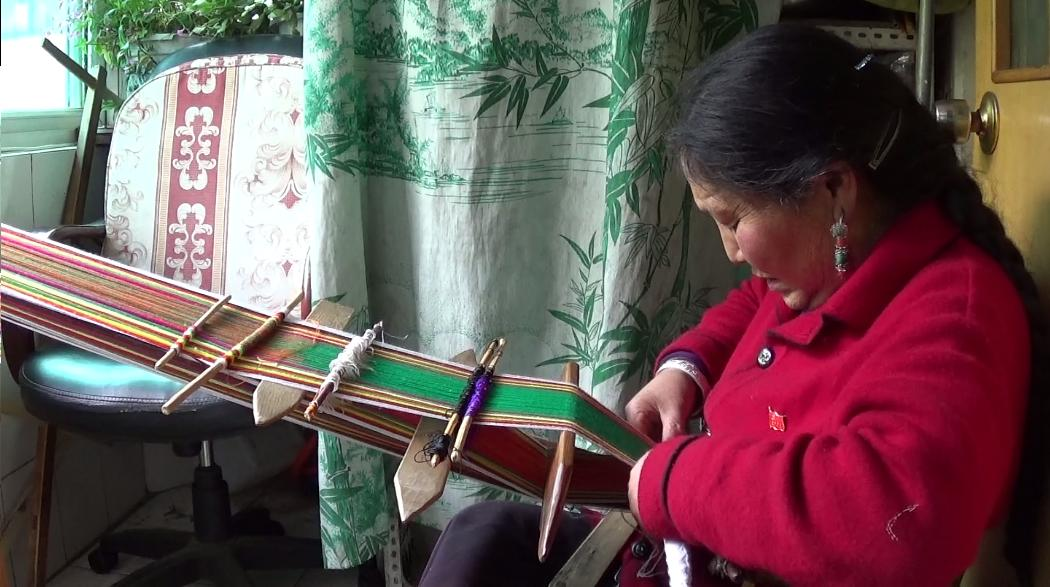
\includegraphics[width=0.8\textwidth]{loom2.jpg}\centering}; %4:20
\tikzstyle{fleche}=[->,very thick,color=green,>=latex]
\tikzstyle{pointille}=[->,dotted,very thick,>=latex]
\begin{scope}[xshift=-0.5cm,rotate=-15]
%    \node[yellow] (A) at (0,1) {up};
%    \node[yellow] (B) at (0,-2.5) {down};
    \node[blue] (C) at (-3,0) {upstream};
    \node[blue] (D) at (3,0) {downstream};
%\draw [fleche] (A)--(B);
\draw [fleche] (C)--(D);
\end{scope}
%\begin{scope}[xshift=-1cm,rotate=15]
%    \node (E) at (-2,-2) {\bleu{eastwards}};
%    \node (F) at (2,2) {\bleu{westwards}};
%    \draw [pointille] (E)--(F);
%\end{scope}
\end{tikzpicture}
\end{figure}

The downstream preverbs are required on all verbs expressing motion towards the lower side, for instance to express the tamping of the intersections between the threads (using the tool called \forme{tʰaʁmu}, which is located between upper and lower warp threads to maintain them apart from each other in \figref{fig:loom1}) towards the waist of the weaver, as in (\ref{ex:thari.chWGnda}).

 \begin{exe}
\ex \label{ex:thari.chWGnda}
\gll ɯ-sqar nɯ tʰɯ-ari tɕe tɕe, nɤki, kɯki tú-wɣ-stu tɕe cʰɯ́-wɣ-ɣnda. \\
\textsc{3sg}.\textsc{poss}-intersection.of.warp.threads \textsc{dem} \textsc{aor}:\textsc{downstream}-go[II] \textsc{lnk} \textsc{lnk} \textsc{filler} \textsc{dem}.\textsc{prox} \textsc{ipfv}-\textsc{inv}-do.like \textsc{lnk} \textsc{ipfv}:\textsc{downstream}-\textsc{inv}-tamp \\
\glt `As the intersection of the [upper and lower] warp threads goes down, one does this to tamp it down.' (vid-20140429090403) \japhdoi{0003776\#S57}
\end{exe} 

The axis that is perpendicular to that of the warp threads and parallel to the ground, through which the weft is inserted (the action depicted in \figref{fig:loom1}), is described using the solar dimension, as shown by the selection of the \textsc{westwards} preverb in (\ref{ex:tWjlAB.YWwGrRe}).

\begin{exe}
\ex \label{ex:tWjlAB.YWwGrRe}
\gll ɯ-taʁ cʰo ɯ-pa ɣɯ ɯ-ʁjar ni pjɯ-ɤqɤtʂʰa-ndʑi, nɯtɕu tɯ-jlɤβ ɲɯ́-wɣ-rʁe tɕe   \\
\textsc{3sg}.\textsc{poss}-top \textsc{comit} \textsc{3sg}.\textsc{poss}-bottom \textsc{gen} \textsc{3sg}.\textsc{poss}-warp \textsc{du} \textsc{ipfv}-be.crossed-\textsc{du} \textsc{dem}.\textsc{loc} \textsc{indef}.\textsc{poss}-weft \textsc{ipfv}:\textsc{west}-\textsc{inv}-insert \textsc{lnk} \\
\glt `The upper and lower warp threads are crossed, and at [the crossing place] one inserts the weft.' (additional explanation provided while transcribing the video from which \figref{fig:loom1} is taken).%vid-20140429090403
\japhdoi{0003776\#S48}
\end{exe} 

The vertical dimension preverbs refer to the third axis that is perpendicular with the two previous ones, with the \textsc{downwards} orientation towards the ground. The \textsc{upwards} preverbs occur to describe the lifting of the warp threads using the heddles, as in (\ref{ex:Cnat.kW.tuwGsWjoR}).

\begin{exe}
\ex \label{ex:Cnat.kW.tuwGsWjoR}
\gll ɕnat kɯ tɤ-ri ra tɕe nɯ kɯ tú-wɣ-sɯ-joʁ tɕe,\\
heddle \textsc{erg} \textsc{indef}.\textsc{poss}-thread \textsc{pl} \textsc{lnk} \textsc{dem} \textsc{erg} \textsc{ipfv}:\textsc{up}-\textsc{inv}-\textsc{caus}-raise \textsc{lnk} \\
\glt `One lifts the [warp] threads with the heddles.' (2011-06-thaXtsa)
\end{exe}  
%{ex:Cnat.maNthi}

\subsection{Lexicalized orientations} \label{sec:lexicalized.orientation}
A complete description of the lexicalized orientation preverbs in Japhug would require a monograph-length treatment taking into account all verbs, basic and derived, and including complex predicates. In order to keep this chapter within a reasonable size, I therefore only focus on a few selected semantic categories comprising the most common non-orientable verbs of the language.

\subsubsection{Spatial use of preverbs with non-orientable verbs} \label{sec:orientation.position}
While non-orientable verbs generally select only one or two orientations (§\ref{sec:lexicalized.orientation}), orientation preverbs that are different from the lexical ones can occur in specific contexts to indicate either a motion event linked with the action of the verb (normally with an additional associated motion prefix, §\ref{sec:orientation.AM}), the motion of a body part or the position of the body. 

The intransitive verb \japhug{cɯ}{hibernate} provides an interesting example of this use of the preverbs. The lexically selected orientation of this verb is \textsc{eastwards} (like other verbs from the same semantic category), as shown by the preverb \forme{ku-} in (\ref{ex:qartsW.tCe.kucW}).

\begin{exe}
\ex \label{ex:qartsW.tCe.kucW}
\gll  qartsɯ tɕe ku-cɯ ɲɯ-ŋu. \\
winter \textsc{loc} \textsc{ipfv}-hibernate \textsc{sens}-be \\
\glt `In winter, [the bear] hibernates.' (21-pri) \japhdoi{0003580\#S49}
\end{exe}

However, the orientations \textsc{upstream} and \textsc{upwards} are also attested with this verb, with more specific readings. The \textsc{upstream} orientation is found in (\ref{ex:praRpa.WNgW.lucW}) and also in (\ref{ex:luCe.tCe.lucW}) above, §\ref{sec:am.prefixes}, and expresses hibernation in a cave. These examples reflect the illative use of the \textsc{upstream} preverbs (§\ref{sec:illative.elative}). The \textsc{upwards} orientation, also shown by (\ref{ex:praRpa.WNgW.lucW}), is used when hibernation takes place in a hollow tree, with vertical motion up the tree (§\ref{sec:vertical.dimension}).

\begin{exe}
\ex \label{ex:praRpa.WNgW.lucW}
\gll tɕe qartsɯ tɕe nɯnɯ si kʰoŋrɤl tɤ-kɯ-ɤri nɯ ɯ-ŋgɯ nɯmaʁ tu-cɯ, 
nɯmaʁnɤ, praʁpa ɯ-ŋgɯ lu-ɕe tɕe lu-cɯ. \\
\textsc{lnk} winter \textsc{loc} \textsc{dem} wood hollow.tree \textsc{aor}:\textsc{up}-\textsc{sbj}:\textsc{pcp}-go[II] \textsc{dem} \textsc{3sg}.\textsc{poss}-in otherwise \textsc{ipfv}:\textsc{up}-hibernate otherwise cave \textsc{3sg}.\textsc{poss}-in \textsc{ipfv}:\textsc{upstream}-go \textsc{lnk} \textsc{ipfv}:\textsc{upstream}-hibernate \\
\glt `In winter, it either hibernates in a hollow tree, or goes into a cave and hibernates (there).' (21-pri)
\japhdoi{0003580\#S100}
\end{exe}

%stu mɤmu nɯ iɕqʰa si kʰoŋrɤl tɤ-kɯ-ɤri 

The forms with \textsc{upstream} and \textsc{upwards} preverbs often occur with either motion verbs or associated motion prefixes, as in (\ref{ex:si.WNgW.tAkWso.WNgW.CtucW}).

\begin{exe}
\ex \label{ex:si.WNgW.tAkWso.WNgW.CtucW}
\gll  si ɯ-ngɯ tɤ-kɯ-so, ɯ-ŋgɯ tɤ-kɯ-rom, nɯnɯ pjɯ-saχsi tɕe, nɯ ɯ-ŋgɯ ɕ-tu-cɯ ɲɯ-ŋu.\\
wood \textsc{3sg}.\textsc{poss}-in \textsc{ipfv}:\textsc{up}-\textsc{sbj}:\textsc{pcp}-be.hollow \textsc{3sg}.\textsc{poss}-in \textsc{ipfv}:\textsc{up}-\textsc{sbj}:\textsc{pcp}-be.dried \textsc{dem} \textsc{ipfv}-do.completely \textsc{lnk} \textsc{dem} \textsc{3sg}.\textsc{poss}-in \textsc{tral}-\textsc{ipfv}:\textsc{up}-hibernate \textsc{sens}-be \\
\glt `Trees whose inside is hollow, whose inside is dried out, [the bear] hollows it completely, goes up [the hole] and hibernates there.' (21-pri) \japhdoi{0003580\#S53}
\end{exe}

The use of preverbs to express spatial position or motion as in the case of the \textsc{upstream} and \textsc{upwards} orientations with \japhug{cɯ}{hibernate} above are not unusual with non-orientable verbs, but are lexicalized, and restricted to highly specific and well-identified situations. Only orientations that are pragmatically and culturally plausible and compatible with the speaker's knowledge of the world can be used: with \japhug{cɯ}{hibernate} for instance, the other series of  orientation preverbs (\textsc{downwards}, \textsc{downstream}, \textsc{westwards}) are not attested. It is not possible to predict which non-orientable verb will be compatible with the spatial use of preverbs, and this information has to be specified in dictionaries in a systematic way. The following sections (§\ref{sec:preverb.ingestion} to §\ref{sec:preverb.cover}) present a series of examples of similar phenomena.
%ɕɤxɕo tɯ-mpja tha-ʑa, tɤjpa pa-lɤt kɯnɤ, pjɯ-lɤt ɯkʰɯkʰa ʑo pjɯ-ndʐi ɲɯ-ɕti wo.

\subsubsection{Preverbs and lability} \label{sec:orientation.lability}
A handful of labile verbs select different preverbs and have slightly different meanings in their transitive and intransitive/semi-transitive uses.

The verb \japhug{sɤŋo}{listen} takes the \textsc{westwards} preverbs when semi-transitive, and the \textsc{eastwards} preverbs when transitive with the meaning `listen to, obey' (§\ref{sec:semi.tr.labile}).  

The verb \japhug{sɯso}{think} is normally transitive and selects the \textsc{westwards} preverbs. It can also occurs with the \textsc{downwards} preverbs, but in this case it is intransitive, and means `in $X$'s opinion' (§\ref{sec:labile.tr-intr}). 

\subsubsection{Irregular orientations with local toponyms} \label{sec:local.toponyms.orientation}
Motion from one locality to another is nearly always expressed using the vertical, riverine and solar dimensions in their basic spatial functions (§\ref{sec:vertical.dimension}, §\ref{sec:riverine.dimension} and §\ref{sec:solar.dimension}, respectively). While in some cases there are conflicts between several possible orientations, especially between the riverine and the solar preverbs, the choice of the preverbs is nearly always motivated.

However, there are also cases where the choice of the preverbs is unrelated to the actual spatial orientation of the trip from one particular place to another. For instance, Kamnyu \forme{kɤmɲɯ} (\href{https://geohack.toolforge.org/geohack.php?params=32.21181437468092_N_101.96170811415986_E}{32° 12′ 43″ N, 101° 57′ 42″ E}) is located to the west of Mengi \forme{mɯŋi} (\href{https://geohack.toolforge.org/geohack.php?params=32.20892642316477_N_102.00383911415355_E}{32° 12′ 32″ N, 102° 0′ 14″ E}, \zh{蒙岩}). 

However, the preverbs corresponding to orientations that are exactly opposite to the geographical orientations are used between these two villages: the orientation \textsc{westwards} is used for motion from Kamnyu to Mengi (to describe a trip from west to east), and \textsc{eastwards} from Mengi to Kamnyu (whereas the actual trip is from east to west), as shown by (\ref{ex:kAmYW.mWNi}) and (\ref{ex:mWNi.YWsAxCe}).

\begin{exe}
\ex \label{ex:kAmYW.mWNi}
\gll kɤmɲɯ tɕe tɕe mɯŋi kɤ-ɕe tɤ-ra tɕe, ``mɯŋi ɲɯ-ɕe-a" tu-kɯ-ti ŋu.
tɕe mɯŋi tɕe kɤmɲɯ nɯ tɕe tɕe, nɤki, ``kɤmɲɯ kɤ-ɣe-a, kɤmɲɯ ku-ɕe-a ŋu" nɯra tu-ti-nɯ. \\
\textsc{topo} \textsc{loc} \textsc{lnk}  \textsc{topo} \textsc{inf}-go \textsc{aor}-be.needed \textsc{lnk}  \textsc{topo} \textsc{ipfv}:\textsc{west}-go-\textsc{1sg} \textsc{ipfv}-\textsc{genr}:S/O-say be:\textsc{fact} \textsc{lnk}  \textsc{topo} \textsc{loc}  \textsc{topo} \textsc{dem} \textsc{lnk} \textsc{lnk} \textsc{filler}  \textsc{topo} \textsc{aor}:\textsc{east}-come[II]-\textsc{1sg} pl.n \textsc{ipfv}:\textsc{east}-go-\textsc{1sg} be:\textsc{fact} \textsc{dem}:\textsc{pl} \textsc{ipfv}-say-\textsc{pl} \\
\glt `When one has to go from Kamnyu to Mengi, one says `I am going (westwards) to Mengi, and from Mengi to Kamnyu, people say `I came (eastwards)  to Kamnyu, I am going (eastwards) to Kamnyu.' (150904 akW andi)
\japhdoi{0006372\#S6}
\end{exe}

\begin{exe}
\ex \label{ex:mWNi.YWsAxCe}
\gll mɯŋi ɲɯ-sɤx-ɕe tʂu nɯnɯre ri, \\
\textsc{topo} \textsc{ipfv}:\textsc{west}-\textsc{obl}:\textsc{pcp}-go path \textsc{dem}:\textsc{loc} \textsc{loc} \\
\glt `On the road (from Kamnyu) towards Mengi...' (140522 Kamnyu zgo) \japhdoi{0004059\#S2}
\end{exe}

This contradiction is clear in example (\ref{ex:akW.mWNi}), where Mengi is explicitly described as being located on the \forme{akɯ} (east) side of Kamnyu.

\begin{exe}
\ex \label{ex:akW.mWNi}
\gll akɯ pɕoʁ nɯ mɯŋi ŋu, andi pɕoʁ praʁwɯ ŋu. \\
 east side \textsc{dem}  \textsc{topo} be:\textsc{fact} west side  \textsc{topo} be:\textsc{fact} \\
\glt `Mengi is in the east, and Praqwu (a small locality in Kamnyu) is in the west.' (140522 Kamnyu zgo) \japhdoi{0004059\#S21}
\end{exe}

Ercha village (in Japhug \forme{ɣɟɯ tsʰapa}, most often called using its Chinese name \zh{二茶村} \forme{èrchácūn}, \href{https://geohack.toolforge.org/geohack.php?params=32.219530245125554_N_101.93203109826473_E}{32° 13′ 10″ N, 101° 55′ 55″ E}), 

located to the west of Kamnyu, also presents orientation inversion: as shown by (\ref{ex:erchacun.kukWCe}), the \textsc{eastwards} preverbs are used for trips from Kamnyu to Ercha, and the \textsc{westwards} preverbs for the opposite trip. This fact has been rechecked with several speakers (note in particular the anecdote reported in §\ref{sec:MBChCh.Dpalcan}).

In (\ref{ex:erchacun.kukWCe}) Tshendzin hesitates: she was about to say \forme{ɲɯ-kɯ-ɕe} with a \textsc{westwards} preverb (the expected form, based on the geographical location of these localities), followed by the the correct \forme{ku-kɯ-ɕe} with the irregular orientation.

\begin{exe}
\ex \label{ex:erchacun.kukWCe}
\gll tɕe kɤmɲɯ tɕe tɕe <erchacun> ɲɯ-kɯ... ku-kɯ-ɕe tɕe tɕe, nɯnɯ ``ku-ɕe-a" tu-kɯ-ti ŋu. <erchacun> tɕe kɤmɲɯ a-nɯ-ɣi-nɯ tɕe nɯ `kɤmɲɯ nɯ-ari-a, kɤmɲɯ nɯ-ɣe-a" nɯra tu-ti-nɯ ŋu. \\
\textsc{lnk}  \textsc{topo} \textsc{loc} \textsc{lnk}  \textsc{topo} { } \textsc{ipfv}:\textsc{east}-\textsc{genr}:S/O-go \textsc{lnk} \textsc{lnk} \textsc{dem} \textsc{ipfv}:\textsc{east}-go-\textsc{1sg} \textsc{ipfv}-\textsc{genr}:S/O-say be:\textsc{fact}  \textsc{topo} \textsc{loc}  \textsc{topo} \textsc{irr}-\textsc{pfv}:\textsc{west}-come-\textsc{pl} \textsc{lnk} \textsc{dem}  \textsc{topo} \textsc{aor}:\textsc{west}-go[II]-\textsc{1sg}  \textsc{topo} \textsc{aor}:\textsc{west}-come[II]-\textsc{1sg}  \textsc{dem}:\textsc{pl} \textsc{ipfv}-say-\textsc{pl} be:\textsc{fact} \\
\glt `When one goes from Kamnyu to Erchacun, one says `I go (eastwards)', and when people come to Kamnyu from Erchacun, they says `I went, I came (westwards).'
(150904 akW andi)
\japhdoi{0006372\#S9}
\end{exe}

This puzzling irregularity has not been observed for other toponyms, especially those located further away from Kamnyu. For instance, the \textsc{upstream} orientation is used for trips to Tshobdun and Zbu, the \textsc{downstream} orientation to Mbarkham (§\ref{sec:riverine.dimension}) and the \textsc{eastwards} orientation to Sarndzu and Tatshi (§\ref{sec:solar.dimension}).


\subsubsection{Verbs of ingestion} \label{sec:preverb.ingestion}
The most common verb of ingestion, \japhug{ndza}{eat}, generally selects the \textsc{upwards} preverbs, as shown for instance by (\ref{ex:chWnWtsWm.Ctundze}) (in §\ref{sec:AM.goal}) and (\ref{ex:nWtCu.Ctundze}) (in §\ref{sec:nature.of.motion.AM}). The same is true of verbs derived from it, such as the compound verb \japhug{rɯndzɤtsʰi}{have a meal} (§\ref{sec:denom.compound.verbs}), as shown by (\ref{ex:ri.CtArWndzAtshij}) in §\ref{sec:AM.goal}, and of other more specialized verbs of food ingestion such as \japhug{moʁ}{eat (powdery food)}, \japhug{nɯtɕʰaʁ}{eat fodder (of horses)}, \japhug{nɯtʂʰɤɣndʑɤr}{eat a tsampa meal}, \japhug{zmɤrɤβ}{eat (mixing with)} or \japhug{χsɤl}{eat (honorific)}.

The \textsc{downstream} preverbs can occur with \japhug{ndza}{eat} to refer to eating by wild beasts and birds of prey, as in (\ref{ex:kWrtsAG.nW.kW.chWndze}), probably due to the fact that this orientation is also selected by \japhug{ɕkɯt}{eat/drink completely}, a verb which can also describe the actions of ferocious animals as in example (\ref{ex:khu.kW.thaCkWt}) in §\ref{sec:obviation.animacy}.\footnote{See also the discussion on the use of the \textsc{downstream} orientation with \japhug{tsʰi}{drink} below, above example \ref{ex:cha.ntsW.chWtshi}).}

\begin{exe}
\ex \label{ex:kWrtsAG.nW.kW.chWndze}
\gll kɯrtsɤɣ nɯ kɯ, nɤki, tɯrme ra ɣɯ nɯ-fsapaʁ nɯ cʰɯ-ndze, [...] qaʑo tsʰɤt nɯ cʰɯ-ndze pjɤ-ŋu, \\
leopard \textsc{dem} \textsc{erg} \textsc{filler} people \textsc{pl} \textsc{gen} \textsc{3pl}.\textsc{poss}-animal \textsc{dem} \textsc{ipfv}:\textsc{downstream}-eat[III] { } sheep goat \textsc{dem} \textsc{ipfv}:\textsc{downstream}-eat[III] \textsc{ifr}.\textsc{ipfv}-be \\
\glt `The snow leopard was eating farm animals, eating ...., sheep and goats.' (qala kWCqraR 2002)
\end{exe}

This orientation is also attested to describe the eating of earth by earthworm as in (\ref{ex:qandzxe.nW.kW.chWndze}), though in this case the preverb is used spatially (§\ref{sec:orientation.position}), reflecting the burrowing motion of the earthworm (§\ref{sec:illative.elative}). 

\begin{exe}
\ex \label{ex:qandzxe.nW.kW.chWndze}
\gll tɕeri qandʐe kɯ tʰɤlwa ʁɟa cʰɯ-ndze ɲɯ-ɕti. \\
\textsc{lnk} earthworm \textsc{erg} earth completely \textsc{ipfv}:\textsc{downstream}-eat[III] \textsc{sens}-be.\textsc{aff} \\
\glt  `The earthworm only eats earth.' (25-akWzgumba)
\japhdoi{0003632\#S115}
\end{exe}

The \textsc{eastwards} orientation is exclusively attested with \forme{ndza} to describe eclipses, as in (\ref{ex:mWkarCo.mACtsxa.kundze}), also a spatial use of the preverbs (expressing motion from the left side to the right side or vice-versa, §\ref{sec:centripetal.centrifugal}).

\begin{exe}
\ex \label{ex:mWkarCo.mACtsxa.kundze}
\gll ɯ-rkɯ kɯ-fse ku-ʑe tɕe, mɯ-kɤ-arɕo mɤɕtʂa ku-ndze ɣɤʑu, \\
\textsc{3sg}.\textsc{poss}-side \textsc{sbj}:\textsc{pcp}-be.like \textsc{ipfv}:\textsc{east}-being[III] \textsc{lnk} \textsc{neg}-\textsc{aor}:\textsc{east}-be.finished until \textsc{ipfv}:\textsc{east}-eat[III] exist:\textsc{sens} \\
\glt  `Sometimes [the eclipse] starts on one side, and `eats' [the moon] until it [disappears] completely.' (29-mWBZi)
\japhdoi{0003728\#S138}
\end{exe}

The orientation \textsc{westwards} occurs with verbs referring to animals eating grass, such as the intransitive verb \japhug{nɯrɯ}{eat grass} as in (\ref{ex:YWnWrWnW}) and its synonym \forme{nɯsɤlɤɣ}.

\begin{exe}
\ex \label{ex:YWnWrWnW}
\gll  nɯŋa qʰe qaʑo tsʰɤt nɯra pjɤ-dɤn-nɯ tɕe, nɯtɕu ɲɯ-nɯrɯ-nɯ tɕe sɯjno tu-ndza-nɯ pjɤ-ŋu, \\
cow \textsc{lnk} sheep goat \textsc{dem}:\textsc{pl} \textsc{ifr}.\textsc{ipfv}-be.many-\textsc{pl} \textsc{lnk} \textsc{dem}:\textsc{loc} \textsc{ipfv}:\textsc{west}-eat.grass-\textsc{pl} \textsc{lnk} grass \textsc{ipfv}:\textsc{up}-eat-\textsc{pl} \textsc{ifr}.\textsc{ipfv}-be \\
\glt  `There were many cows, sheep and goats, and they were eating grass there.' (150819 woniu-zh)
\japhdoi{0006254\#S8}
\end{exe}

Verbs related to the ingestion of liquids select the \textsc{eastwards} preverbs as default, as in (\ref{ex:konWkhWG.Zo.kotshi}), including the deideophonic \japhug{nɯkʰɯɣ}{gulp} (§\ref{sec:nW.deidph}).

\begin{exe}
\ex \label{ex:konWkhWG.Zo.kotshi}
\gll tɯ-ci ko-nɯkʰɯɣ ʑo ko-tsʰi. \\
\textsc{indef}.\textsc{poss}-water \textsc{ifr}:\textsc{east}-gulp \textsc{emph} \textsc{ifr}:\textsc{east}-drink \\
\glt `He gulped the water.' (140429 jiedi-zh)
\end{exe}

The verb \japhug{tsʰi}{drink} is also found with the \textsc{downwards} orientation to refer to drinking with the head down on the grounds (like animals, or from a jar with a straw), for instance in (\ref{ex:GWpjWnWtshinW}) and (\ref{ex:CpjAnWtshi}) in §\ref{sec:am.prefixes} and (\ref{ex:WtAlu}) in §\ref{sec:alienabilization}. The denominal verb \japhug{nɯci}{drink from the ground} also selects this orientation.

The \textsc{downstream} preverbs occur with this verb in two contexts. First,  following the basic spatial meaning of these preverbs (`direction of the flow of water', §\ref{sec:riverine.dimension}), they can be used to insist on the flow of liquid through the oesophagus during ingestion, as in (\ref{ex:tWci.chWtshi}). 

\begin{exe}
\ex \label{ex:tWci.chWtshi}
\gll tɯ-ci kɯnɤ cʰɯ-ɕe mɯ-ɲɤ-kʰɯ. tɯ-ci cʰɯ-tsʰi mɯ-ɲɤ-kʰɯ \\
\textsc{indef}.\textsc{poss}-water also \textsc{ipfv}:\textsc{downstream}-go \textsc{neg}-\textsc{ifr}-be.possible \textsc{indef}.\textsc{poss}-water \textsc{ipfv}:\textsc{downstream}-drink \textsc{neg}-\textsc{ifr}-be.possible \\
\glt `Even water could not go [down his throat], he could not drink anymore.' (of a person suffering from throat cancer) (27-tWfCAl) \japhdoi{0003710\#S87}
\end{exe}

Second, the \textsc{downstream} orientation is found to express excessive alcohol drinking, as in (\ref{ex:cha.ntsW.chWtshi}), possibly by analogy with \japhug{ɕkɯt}{eat/drink completely} which also takes this orientation (see also the discussion concerning example \ref{ex:kWrtsAG.nW.kW.chWndze} above).

\begin{exe}
\ex \label{ex:cha.ntsW.chWtshi}
\gll  ɯ-wa nɯ kɯ cʰa ntsɯ cʰɯ-tsʰi qʰe, ɯ-me mɯ́j-nɯβdaʁ \\
\textsc{3sg}.\textsc{poss}-father \textsc{dem} \textsc{erg} alcohol always \textsc{ipfv}:\textsc{downstream}-drink \textsc{lnk} \textsc{3sg}.\textsc{poss}-daughter \textsc{neg}:\textsc{sens}-take.care \\
\glt `Her father was drinking alcohol all the time, and did not take care of his daughter.' (17-lhazgron)
\end{exe}

The \textsc{downstream} preverbs are also selected by the denominal verb \japhug{nɯcʰɤmda}{drink with a straw} (example \ref{ex:chWwGnWchAmdaj}, §\ref{sec:svc}), probably reflecting the illative (through tubular opening) function of the \textsc{downstream} preverb (§\ref{sec:illative.elative}). It is noteworthy that \japhug{tsʰi}{drink} takes the \textsc{downwards} orientation instead when referring to drinking from a straw.

%\japhug{aʁe}{get to eat} {sec:preverb.gain}

The \textsc{upstream} preverbs occur with the verb \forme{χɤβ}, which can mean `drink until the last drop in one gulp', or `breathe in, suck up, draw up' as in (\ref{ex:WsnWro.luXAB}), a special case of the illative  (through large opening) function of this orientation (§\ref{sec:illative.elative}; note that the illative is expressed with the opposite orientation as that of \japhug{nɯcʰɤmda}{drink with a straw}, due to the difference of the shape of the opening).

\begin{exe}
\ex \label{ex:WsnWro.luXAB}
\gll ɯ-sŋɯro lu-χɤβ ʑo tɕe nɯ βɣɤza nɯ ɯ-kɯr ɯ-ŋgɯ lu-nɯ-ɕe ɕti \\
\textsc{3sg}.\textsc{poss}-breath \textsc{ipfv}:\textsc{upstream}-suck \textsc{emph} \textsc{dem} \textsc{lnk} fly \textsc{dem} \textsc{3sg}.\textsc{poss}-mouth \textsc{3sg}.\textsc{poss}-in \textsc{ipfv}:\textsc{upstream}-\textsc{auto}-go be.\textsc{aff}:\textsc{fact} \\
\glt `[The frog]$_i$ breathes in and the fly goes into its$_i$ mouth by itself.' (27-qaCpa)
\japhdoi{0003716\#S7}
\end{exe}

\subsubsection{Stative verbs expressing size} \label{sec:preverb.adjectives.size}
Adjectival verbs describing size, like other stative verbs, become dynamic verbs (`become X') in the Imperfective (§\ref{sec:imperfective}), the Irrealis (§\ref{sec:irrealis}), the Aorist (§\ref{sec:aor.inchoative}) and the Inferential (§\ref{sec:ifr}). The most neutral orientation preverbs for these verbs are indicated in \tabref{tab:size.adj.preverbs}. Most positive adjectival verbs select the \textsc{upwards} orientation, except for those describing radial size (\japhug{jpum}{be thick}, \japhug{rɟum}{be broad}) which are  found with the \textsc{westwards} orientation, and those expressing length (see below).

It is much more difficult to ascertain the lexically selected orientation of negative adjectival verbs, since the situations in which their use as dynamic verbs is appropriate (`become small(er)', `become short(er)') are less common. The \textsc{downwards} orientation does occur as lexically selected orientation (with \japhug{xtɕi}{be small}  and \japhug{mbɤr}{be low}), resulting in forms that are homophonous with the Past Imperfective (§\ref{sec:pst.ifr.ipfv}). Perhaps due to this homophony, the \textsc{westwards} orientation is also used instead with \japhug{xtɕi}{be small}, as in (\ref{ex:WCGa.anWxtCi}).

\begin{exe}
\ex \label{ex:WCGa.anWxtCi}
\gll ki ɯ-ʁɤri sɯstaʁ ʑo ɯ-ɕɣa a-nɯ-xtɕi ra \\
\textsc{dem}.\textsc{prox} \textsc{3sg}.\textsc{poss}-before \textsc{comp} \textsc{emph} \textsc{3sg}.\textsc{poss}-age \textsc{irr}-\textsc{pfv}:\textsc{west}-small be.needed:\textsc{fact} \\
\glt `May she become younger than before!' (2005 Norbzang)
\end{exe}

\begin{table}
\caption{Adjectival stative verbs of size and orientation preverbs} \label{tab:size.adj.preverbs}
\begin{tabular}{lllll}
\lsptoprule
Positive size & Orientation & Negative size & Orientation \\
\midrule
\japhug{wxti}{be big} & up & \japhug{xtɕi}{be small} & west, down \\
\japhug{mbro}{be high} & up & \japhug{mbɤr}{be low} & down \\
&&(of size) \\
\japhug{zri}{be long},  & up,  & \japhug{xtɯt}{be short} & west \\
&downstream &&upstream\\
\japhug{rɲɟi}{be long} &&& \\
\japhug{jpum}{be thick}  & west & \japhug{xtsʰɯm}{be thin}& west, east \\
 (of radius)&& (of radius) \\
\japhug{jaʁ}{be thick} & up & \japhug{mba}{be thin} & west  \\
(of a surface)  &&(of a surface) \\
\japhug{rɟum}{be broad}  & west & \japhug{tɕɤr}{be narrow} &  east  \\
&&  \japhug{ŋgɤr}{be narrow} &  east  \\
\lspbottomrule
\end{tabular}
\end{table}

In addition to the orientations in Table (\ref{tab:size.adj.preverbs}), the \textsc{downstream} preverbs can occur to express a progressive increase (§\ref{sec:orientation.preverb.aspect}). Compare for instance the use of \japhug{wxti}{be big} with the \textsc{upwards} orientation in (\ref{ex:Wkha.towxti})  with that in (\ref{ex:ZWrWZAri.chAwxti}) with the \textsc{downstream} orientation, describing a process taking place progressively over many years.

\begin{exe}
\ex \label{ex:Wkha.towxti}
\gll mɤʑɯ ʑo ɯ-kʰa ra to-wxti tɕe, \\
even.more \textsc{emph} \textsc{3sg}.\textsc{poss}-house \textsc{pl} \textsc{ifr}:\textsc{up}-be.big \textsc{lnk} \\
\glt  `His house had become even bigger.' (140430 yufu he tade qizi-zh)
\japhdoi{0003900\#S212}
\end{exe}

\begin{exe}
\ex \label{ex:ZWrWZAri.chAwxti}
\gll tɕeri ɯ-tɕɯ nɯ ʑɯrɯʑɤri cʰɤ-wxti  \\
\textsc{lnk} \textsc{3sg}.\textsc{poss}-son \textsc{dem} progressively \textsc{ifr}:\textsc{downstream}-be.big \\
\glt `His son progressively grew up.' (28-smAnmi)
\japhdoi{0004063\#S10}
\end{exe}

Some of these verbs are compatible with more than one orientation. For instance, \japhug{rɲɟi}{be long} is attested with the \textsc{upwards} orientation to refer to the length of a vertical object, as in (\ref{ex:turYJi.mAcha}) (where it is synonymous with \japhug{mbro}{be high}). With the \textsc{upstream} preverbs, it describes for instance (elongated) fruits or leaves growing out of the branch of a plant, as in (\ref{ex:lurYJi.tsa.Nu}).
 
\begin{exe}
\ex \label{ex:turYJi.mAcha}
\gll tɕe <yimi> jamar ma tu-rɲɟi mɤ-cʰa ma  \\
\textsc{lnk} one.meter about apart.from \textsc{ipfv}:\textsc{up}-be.long \textsc{neg}-can:\textsc{fact} \textsc{lnk} \\
\glt `It cannot grow longer than about one meter.' (11-qarGW)
\japhdoi{0003480\#S98}
\end{exe}

\begin{exe}
\ex \label{ex:lurYJi.tsa.Nu}
\gll tɯrgi ɣɯ ɯ-mat lu-rɲɟi tsa ŋu tɕe, nɤki jima popo tsa fse. \\
fir \textsc{gen}  \textsc{3sg}.\textsc{poss}-fruit \textsc{ipfv}:\textsc{upstream}-be.long a.little be:\textsc{fact} \textsc{lnk} \textsc{filler} maize cob a.little be.like:\textsc{fact} \\
\glt  `The fir cone is elongated, a bit like the corncob (07-tAtho)
\japhdoi{0003432\#S28}
\end{exe}

The \textsc{downstream} preverbs are found to express progressive increase (example \ref{ex:ZWrWZAri.chAwxti}, §\ref{sec:redp.gradual.increase}, §\ref{sec:tense.aspect.adverbs}), as in (\ref{ex:chWxtWt.Nu}), but can also refer to the growth of thread-like objects like hair, as in (\ref{ex:tWkArme.chWrYi}). Note in this example that \japhug{rɤɕi}{pull} shares the same preverb to refer to the pulling of hairs.
 
\begin{exe}
\ex \label{ex:chWxtWt.Nu}
\gll ɕɤr nɯ cʰɯ-rɲɟi, sŋi nɯ cʰɯ-xtɯt ɲɯ-ŋu \\
night \textsc{dem} \textsc{ipfv}:\textsc{downstream}-be.long day \textsc{dem}  \textsc{ipfv}:\textsc{downstream}-be.short \textsc{sens}-be \\
\glt `The nights are becoming longer, and the days shorter.' (elicited)
\end{exe}

\begin{exe}
\ex \label{ex:tWkArme.chWrYi}
\gll pɯ-kɯ-xtɕi tɕe, nɯnɯ ʑŋgri nɯ nɯ-mɤrʑaβ ɯ-raŋ tɕe, tɯ-kɤrme cʰɯ́-wɣ-rɤɕi tɕe, cʰɯ-rɲɟi ŋu to-ti-nɯ tɕe,\\
\textsc{pst}.\textsc{ipfv}-\textsc{genr}:S/O-be.small \textsc{lnk} \textsc{dem} star \textsc{dem}  \textsc{aor}-marry \textsc{3sg}.\textsc{poss}-time \textsc{lnk} \textsc{genr}.\textsc{poss}-hair \textsc{ipfv}:\textsc{downstream}-\textsc{inv}-pull \textsc{lnk} \textsc{ipfv}:\textsc{downstream}-be.long be:\textsc{fact} \textsc{ifr}-say-\textsc{pl} \textsc{lnk} \\
\glt `When we were young, people said that when there is a shooting star, if you pull your hair, it will grow longer.' (29-mWBZi)
\japhdoi{0003728\#S93}
 \end{exe}
%{ex:Wmat.chWkWBze} ku-kɯ-xtsʰɯm ɲɯ-kɯ-jpum 

\subsubsection{Verbs related to growth, gain or birth} \label{sec:preverb.gain}
Adjectival verbs of size can be used to express growth (§\ref{sec:preverb.adjectives.size}), but another constructions expressing the same meaning involves the transitive verb \japhug{βzu}{make} with a dummy subject (§\ref{sec:transitive.dummy}), and an adjectival verb in participial form (§\ref{sec:subject.participles}), as in (\ref{ex:kWmbWmbro.tuBze}), with the \textsc{upwards} orientation (compare with \ref{ex:turYJi.mAcha} above and \ref{ex:YWwGzmaqhu} in §\ref{sec:obviation.animacy}).
 

\begin{exe}
\ex \label{ex:kWmbWmbro.tuBze}
\gll ɕɤɣ nɯ li kɯ-mbɯ\redp{}mbro tu-βze cʰa \\
juniper \textsc{dem} again \textsc{sbj}:\textsc{pcp}-\textsc{emph}\redp{}be.high \textsc{ipfv}:\textsc{up}-make[III] can:\textsc{fact} \\
\glt `The juniper grows very high.' (08-CAG) \japhdoi{0003442\#S1}
 \end{exe}
 
The \textsc{upstream} orientation appears to describe fruits or leaves growing out of a plant, as in (\ref{ex:tWrgi.laNlaN.laBzu})  (compare with \ref{ex:lurYJi.tsa.Nu} above).
 
 \begin{exe}
\ex \label{ex:tWrgi.laNlaN.laBzu}
\gll  tɯrgi laŋlaŋ nɯnɯ, la-βzu ɕimɯma nɯ ɲɯ-ɤrŋi, \\
fir cone \textsc{dem} \textsc{aor}:\textsc{upstream}:3\flobv{}-make immediately \textsc{dem} \textsc{sens}-be.green \\
\glt `The fir cone is green when it has just come out.' (08-tWrgi)
  \end{exe}

The \textsc{downstream} orientation is found with long and thin thread-like objects, like the stalks of some plants as in (\ref{ex:Wru.chWBze}) (compare with \ref{ex:tWkArme.chWrYi}), but also occur to refer to fruits or grains (\ref{ex:Wmat.kWfse.chWBze}), probably as an extension of the progressive incrementation function of this orientation (\ref{ex:ZWrWZAri.chAwxti} above, §\ref{sec:preverb.adjectives.size}).

  \begin{exe}
\ex \label{ex:Wru.chWBze}
\gll   ɯ-ru ra kɯ-xtsʰɯ\redp{}xtsʰɯm ŋu ri, kɯ-zɯ\redp{}zri ʑo cʰɯ-βze qʰe,  \\
  \textsc{3sg}.\textsc{poss}-stalk \textsc{pl} \textsc{sbj}:\textsc{pcp}-\textsc{emph}\redp{}be.thin be:\textsc{fact} \textsc{lnk}  \textsc{sbj}:\textsc{pcp}-\textsc{emph}\redp{}be.long \textsc{emph} \textsc{ipfv}:\textsc{downstream}-make[III] \textsc{lnk} \\
\glt `Although its stalk is very thin, it grows very long.' (19-qachGa mWntoR)
  \end{exe}
  
\begin{exe}
\ex \label{ex:Wmat.kWfse.chWBze}
\gll    sɯŋgɯpɤjka nɯ ɯ-mat nɯnɯ pɤjka kɯ-fse cʰɯ-βze,    \\
wild.squash \textsc{dem} \textsc{3sg}.\textsc{poss}-fruit \textsc{dem} squash \textsc{sbj}:\textsc{pcp}-be.like \textsc{ipfv}:\textsc{downstream}-make[III] \\
\glt `Wild squash grows fruits like those of the [cultivated] squash.' (16-CWrNgo)
\japhdoi{0003518\#S37}
\end{exe}

The intransitive verb \japhug{ndzɤt}{grow} also selects the \textsc{upwards} orientation to describe the growth of a plant, and the \textsc{downstream} preverbs for children, as in (\ref{ex:tApAtso.chondzAt}).

\begin{exe}
\ex \label{ex:tApAtso.chondzAt}
\gll   tɤ-pɤtso cʰo-ndzɤt \\
\textsc{indef}.\textsc{poss}-child \textsc{ifr}:\textsc{downstream}-grow \\
\glt  `The child grew up.' (elicited)
\end{exe}

For growth in quantity rather than size, the \textsc{upwards} orientation is selected, for instance with the verb \japhug{dɤn}{be many} in (\ref{ex:tAdAnnW2}).

\begin{exe}
\ex \label{ex:tAdAnnW2}
\gll  tʰam tɕe mɤʑɯ tɤ-dɤn-nɯ  \\
now \textsc{lnk} even.more \textsc{aor}:\textsc{up}-be.many-\textsc{pl}  \\
\glt `Now they are even more numerous than before.' (140522 tshupa) \japhdoi{0004053\#S84}
\end{exe}

The \textsc{upwards} orientation is also selected by verbs expressing birth and coming into existence such as \japhug{tu}{exist} in (\ref{ex:ci.totu}) and (\ref{ex:tWci.paRea}) (note that its antonym \japhug{me}{not exist} rather selects the \textsc{westwards} orientation, §\ref{sec:preverb.loss}), and verbs of Tibetan origin such as \japhug{sci}{be born} (\ref{ex:WtCW.tosci}) and the honorific \japhug{mkʰroŋ}{be reincarnated} (\ref{ex:GWtomkhroN}).

\begin{exe}
\ex \label{ex:ci.totu}
\gll  ndʑi-tɕɯ ci to-tu \\
3du.\textsc{poss}-son \textsc{indef} \textsc{ifr}:\textsc{up}-exist \\
\glt `They had one son.' (2011-05-nyima)
\end{exe}

\begin{exe}
\ex \label{ex:WtCW.tosci}
\gll ɯ-tɕɯ to-sci ɕi, ɯ-me to-sci? \\
\textsc{3sg}.\textsc{poss}-son \textsc{ifr}-be.born \textsc{qu} \textsc{3sg}.\textsc{poss}-girl \textsc{ifr}-be.born \\
\glt `Did she have a boy or a girl?' (elicited)
\end{exe}

\begin{exe}
\ex \label{ex:GWtomkhroN}
\gll nɯʑora nɯ-ɕki ɣɯ-to-mkʰroŋ ɲɯ-ŋu.  \\
\textsc{2pl} \textsc{2pl}.\textsc{poss}-\textsc{dat} \textsc{cisl}-\textsc{ifr}:\textsc{up}-be.born \textsc{sens}-be \\
\glt `He had come to be born in their [family].' (150825 nezha naohai-zh) \japhdoi{0006272\#S35}
\end{exe}

The \textsc{downstream} orientation however occurs with verbs expressing humans or animals giving birth, such as the intransitive denominal verbs \japhug{rɤpɯ}{have young}, \japhug{rɤŋgɯm}{lay eggs} and \japhug{rɤrɟit}{have a child} (§\ref{sec:denom.intr.rA}) and the light verb \japhug{lɤt}{release} in the meaning `give birth to' in (\ref{ex:thWrApW.chWlAt}). This may be an extension of the elative function of the \textsc{downstream} preverbs (§\ref{sec:illative.elative}).

\begin{exe}
\ex \label{ex:thWrApW.chWlAt}
\gll tsʰɤt nɯ tʰɯ-rɤpɯ tɕe, ʁnɯz ntsɯ cʰɯ-lɤt ŋgrɤl \\
goat \textsc{dem} \textsc{aor}:\textsc{downstream}-have.young \textsc{lnk} two always \textsc{ipfv}:\textsc{downstream}-release be.usually.the.case:\textsc{fact} \\
\glt `When goats have young, they give birth to two [kids] at a time.' (05-qaZo)
\japhdoi{0003404\#S6}
\end{exe}

\begin{exe}
\ex \label{ex:chWrANgWm}
\gll tɯ-ji ɯ-ŋgɯ nɯra cʰɯ-rɤŋgɯm ŋgrɤl \\
\textsc{indef}.\textsc{poss}-field \textsc{3sg}.\textsc{poss}-in \textsc{dem}:\textsc{pl} \textsc{ipfv}:\textsc{downstream}-lay.eggs be.usually.the.case:\textsc{fact} \\
\glt `It lays eggs in the fields.' (24-kWmu) \japhdoi{0003618\#S80}
\end{exe}

Verbs expressing gain select the \textsc{downwards} orientation, including the orientable verb \japhug{mɟa}{take} (§\ref{sec:manipulation.verbs}) when used in the meaning `obtain, get' (example \ref{ex:pjWGmJa.ma.mWpWkWcha} in §\ref{sec:antipassive.t}), \japhug{βɟɤt}{obtain} (§\ref{sec:antipassive.t}), \japhug{mto}{see} (which can mean `find' especially when used with the autive prefix, see §\ref{sec:preverb.perception} and §\ref{sec:autoben.spontaneous}) as well as the semi-transitive \japhug{aʁe}{have to eat/drink}\footnote{This verb can be translated into Chinese as \ch{吃到}{chīdào}{have to eat} or \ch{喝到}{hēdào}{have to drink}.} as in (\ref{ex:tWci.paRea}).
  
\begin{exe}
\ex \label{ex:tWci.paRea}
\gll a-kɯr ɯ-ŋgɯ tɯ-ci pɯ-aʁe-a tɕe, a-sroʁ to-tu  \\
\textsc{1sg}.\textsc{poss}-mouth \textsc{3sg}.\textsc{poss}-in \textsc{indef}.\textsc{poss}-water \textsc{aor}:\textsc{down}-be.needed.eat-\textsc{1sg} \textsc{lnk} \textsc{1sg}.\textsc{poss}-life \textsc{ifr}:\textsc{up}-exist \\
\glt `I have water in my mouth to drink, my life is back.' (2011-05-nyima)
\end{exe} 

\subsubsection{Verbs related to loss or death} \label{sec:preverb.loss}
Verbs expressing loss, with meanings such as `disappear' or `lose' generally select the orientation \textsc{westwards}, probably as an extension of its centrifugal use (§\ref{sec:centripetal.centrifugal}). For instance, the verb \japhug{βde}{throw}, which can also be interpreted as meaning `lose' when used non-volitionally (especially with the autive §\ref{sec:autoben.lexicalized}), selects this orientation, as shown by (\ref{ex:Wrte.YAnWBde}), even though the loss of the hat (in the pear story movie) involved a motion downwards.
 
\begin{exe}
\ex \label{ex:Wrte.YAnWBde}
\gll tɕe ɯ-rte ra ɲɤ-nɯ-βde tɕe, \\
\textsc{lnk} \textsc{3sg}.\textsc{poss}-hat \textsc{pl} \textsc{ifr}:\textsc{west}-\textsc{auto}-lose \textsc{lnk} \\
\glt  `[The boy] lost his hat' (Pear story 2010, Tshendzin,  12)
\end{exe} 

The same is observed with the verb \japhug{me}{not exist} in (\ref{ex:mtshu.YAme}), here also despite a clear downward motion of the water level until the lake disappears.

\begin{exe}
\ex \label{ex:mtshu.YAme}
\gll mtsʰu nɯ cʰɯmcʰɯm ʑo, tɕe, tɯ-skɤm pjɤ-sɤʑa tɕe mtsʰu nɯ ɲɤ-me tɕe \\
lake \textsc{dem} \textsc{idph}(II):slowly \textsc{emph} \textsc{lnk} \textsc{inf}:II-dry.up \textsc{ifr}:\textsc{down}-start \textsc{lnk} lake \textsc{dem} \textsc{ifr}:\textsc{west}-not.exist \textsc{lnk} \\
\glt `The level of the lake started to go down slowly and the lake disappeared.' (nyima2003)
\end{exe} 

Verb expressing partial disappearance, such as \japhug{rkɯn}{be few} in (\ref{ex:si.YWYArkWn}), also occur with the \textsc{westwards} orientation.

\begin{exe}
\ex \label{ex:si.YWYArkWn}
\gll zgoku nɯtɕu si nɯ ʑɯrɯʑɤri ɲɯ\redp{}ɲɤ-rkɯn ʑo \\
mountain \textsc{dem}:\textsc{loc} tree \textsc{dem} progressively \textsc{incr}\redp{}\textsc{ifr}:\textsc{west}-be.few \textsc{emph} \\
\glt `There were fewer and fewer trees on the mountain.' (04-xiaocunzhuang-zh) \japhdoi{0003394\#S24}
\end{exe} 

The verb \japhug{ɕqʰlɤt}{disappear}, also semantically related to these verbs, is an orientable motion verb (§\ref{sec:motion.verbs}). It does not usually select the \textsc{westwards} orientation in a non-spatial way, except for the express the passing of time (§\ref{sec:vertical.preverbs.time}). In example (\ref{ex:tANe.YWCqhlAt}), there is however some ambiguity as to whether the \textsc{westwards} orientation is purely spatial (the setting of the sun in the west, see §\ref{sec:solar.dimension}; note that the vertical dimension is more commonly selected, §\ref{sec:vertical.dimension}), or whether it could also be analyzed as centripetal.
 
\begin{exe}
\ex \label{ex:tANe.YWCqhlAt}
\gll  tɤŋe nɯ ɲɯ-ɕqʰlɤt ku-nɤjɤm ra kʰi ma tɤŋe nɯ wuma ʑo nɯɣ-me kʰi.  \\
sun \textsc{dem} \textsc{ipfv}:\textsc{west}-disappear \textsc{ipfv}-wait[III] be.needed:\textsc{fact} hearsay \textsc{lnk} sun \textsc{dem} really \textsc{emph} \textsc{appl}-be.afraid[III]:\textsc{fact} hearsay \\
\glt `[The yeti] waits for the sun to disappear [before eating the man he has caught], because he fears the sun, it is said.' (140510 mYWrgAt)
\japhdoi{0003941\#S7}
\end{exe} 

It is possible that the centripetal function of the \textsc{westwards} orientation has originated from a metaphoric extension of the disappearance of the sun in the west at dusk, in which examples like (\ref{ex:tANe.YWCqhlAt}) would be the pivot construction allowing reanalysis from a purely spatial marker to a more abstract meaning such as `away from the deictic center' or `loss'.

Verbs expressing a more abstract type of disappearance, such as the cognition verb \japhug{jmɯt}{forget} (memory loss), likewise select the \textsc{westwards} prefixes, as in \forme{ɲɤ-nɯ-jmɯt-a} \textsc{ifr}:\textsc{west}-\textsc{auto}-forget-\textsc{1sg} `I forgot (about it)' (see \ref{ex:mAxsi.YAnWjmWta}, §\ref{sec:1.genr}).

The verb \japhug{me}{not exist} has another set of forms with the \textsc{upwards} orientation, as in (\ref{ex:si.tAme}). With the \textsc{upwards} vertical preverbs, this verb does not entail the presupposition that loss occurred; in the perfective, the \forme{tɤ-me} with \textsc{upwards} orientation means `when there this no X' (a usage found with other stative verbs, §\ref{sec:orientation.preverb.aspect}), while \forme{nɯ-me} with \textsc{westwards} orientation can only be interpreted as `(when) X disappeared/was lost'.

 \begin{exe}
\ex \label{ex:si.tAme}
\gll  nɯ ma si tɤ-me tɕe li nɯ ɲɯ-pʰɯt-nɯ\\
\textsc{dem} apart.from wood \textsc{aor}:\textsc{up}-not.exist \textsc{lnk} again \textsc{dem} \textsc{ipfv}-take.out-\textsc{pl}\\
\glt `When there is no other wood than this, people cut it.' (07-Zmbri)
\japhdoi{0003438\#S59}
\end{exe} 

As in many languages (for instance Indo-European \forme{*mer}, \citealt[439--440]{liv}), \forme{me} in the meaning `disappear' is commonly used as a euphemism for passing away, as in (\ref{ex:WXti.YAme}).

 \begin{exe}
\ex \label{ex:WXti.YAme}
\gll  ɯʑo ɯ-χti ɲɤ-me tɕe,  \\
\textsc{3sg} \textsc{3sg}.\textsc{poss}-companion \textsc{ifr}:\textsc{west}-not.exist \textsc{lnk} \\
\glt `Her husband passed away.' (12-BzaNsa) \japhdoi{0003484\#S111}
\end{exe} 

Likewise, verbs expressing death and destruction, such as \japhug{si}{die} and \japhug{χɕaʁ}{pass away} (a borrowing from \tibet{གཤེགས་}{gɕegs}{go away}), \japhug{plɯt}{destroy}, \japhug{ndʑɯɣ}{be destroyed} select the \textsc{westwards} orientation, as shown by (\ref{ex:tongo.YAsi}), (\ref{ex:WrGi.nWplWti}) and (\ref{ex:Ctusci.YWNu}) further below (in §\ref{sec:nature.of.motion.AM}).

 \begin{exe}
\ex \label{ex:tongo.YAsi}
\gll βdaʁmu nɯ to-ngo tɕe ɲɤ-si. \\
lady \textsc{dem} \textsc{ifr}-be.ill \textsc{lnk} \textsc{ifr}:\textsc{west}-die \\
\glt `The lady became ill and died.' (2011-05-nyima)
 \end{exe} 
 
  \begin{exe}
\ex \label{ex:WrGi.nWplWti}
\gll  jima ɯ-rɣi nɯ-plɯt-i \\
maize \textsc{3sg}.\textsc{poss}-grain \textsc{aor}:\textsc{west}-destroy-\textsc{1pl} \\
\glt `We have used up all the maize grains.' (elicited)
  \end{exe} 
  
 The verb \japhug{si}{die} alternatively also occur with the \textsc{downwards} preverbs, in particular in the case of animals as in (\ref{ex:nWNGarmW.pjAsi}). With humans, using the \textsc{downwards} preverbs is not rude, but considered to be blunter than with the  westwards' preverbs.
 
\begin{exe}
\ex \label{ex:nWNGarmW.pjAsi}
\gll  tɕetu ʑara nɯ-ɴɢarmɯ nɯ pjɤ-si kʰi tɕe,  \\
up.there \textsc{3pl} \textsc{3pl}.\textsc{poss}-hybrid.cow \textsc{dem} \textsc{ifr}:\textsc{down}-die hearsay \textsc{lnk} \\
\glt `Those up there, their cow died, it is said.' (Tagrdo conversation, 2003)
   \end{exe} 
   
The transitive verb \japhug{sat}{kill} also selects the \textsc{downwards} orientation preverbs, even when taking an associated motion prefix and an overt goal pointing to an orientation other than \textsc{downwards}, as in (\ref{ex:pGAtCW.CpWsatnW}).

\begin{exe}
\ex \label{ex:pGAtCW.CpWsatnW}
\gll  atu pɣɤtɕɯ nɯ ɕ-pɯ-sat-nɯ ra \\
up.there bird \textsc{dem} \textsc{tral}-\textsc{imp}:\textsc{down}-kill-\textsc{pl} be.needed:\textsc{fact} \\
\glt `Go and kill the bird up there.' (2005 Kunbzang)
   \end{exe} 
   
Likewise, \japhug{ntɕʰa}{kill, butcher} (on whose etymology see \citealt[303--309]{gong18these}) occurs with the \textsc{downwards} preverbs in the meaning `kill (an animal)', as shown by (\ref{ex:nWNa.pjAnWnWntChanW}). 

\begin{exe}
\ex \label{ex:nWNa.pjAnWnWntChanW}
\gll  tɕe nɯ-nɯŋa pjɤ-nɯ-ntɕʰa-nɯ \\
\textsc{lnk} \textsc{3pl}.\textsc{poss}-cow \textsc{ifr}:\textsc{down}-\textsc{auto}-butcher-\textsc{pl} \\
\glt `They killed their cow (for themselves to eat).' (02-deluge2012) \japhdoi{0003376\#S16}
\end{exe} 

The orientation \textsc{westwards} also occurs with this verb in the meaning `butcher', as illustrated by (\ref{ex:natChanW.tutCAtnW}) and (\ref{ex:YWtChanW}). On the other hand, \japhug{sat}{kill} is not found with the \textsc{westwards} preverbs.

\begin{exe}
\ex \label{ex:natChanW.tutCAtnW}
\gll fsapaʁ ɯ-ŋgru pɯ-nɯ-ŋu, rɯdaʁ ɯ-ŋgru pɯ-nɯ-ŋu,  nɯnɯ na-ntɕʰa-nɯ tɕe tu-tɕɤt-nɯ tɕe tɕe tu-sɯɣ-rom-nɯ. \\
farm.animals \textsc{3sg}.\textsc{poss}-sinew  \textsc{pst}.\textsc{ipfv}-\textsc{auto}-be  \textsc{3sg}.\textsc{poss}-sinew  wild.animals \textsc{pst}.\textsc{ipfv}-\textsc{auto}-be \textsc{dem} \textsc{aor}:\textsc{west}:3\flobv{}-butcher-\textsc{pl} \textsc{lnk} \textsc{ipfv}:\textsc{up}-take.out-\textsc{pl} \textsc{lnk} \textsc{lnk} \textsc{ipfv}-\textsc{caus}-be.dry-\textsc{pl} \\
\glt `Whether it is sinew$_i$ from a farm or a wild animal,$_j$  after they butcher them,$_j$ they take it$_i$ out and dry it$_i$.' (150906 tWNgru) \japhdoi{0006304\#S5}
\end{exe} 

\begin{exe}
\ex \label{ex:YWtChanW}
\gll nɯnɯ pa-sat-nɯ tɕe tɕe ju-nɯ-ɣɯt-nɯ tɕe ɲɯ-ntɕʰa-nɯ  \\
\textsc{dem} \textsc{aor}:\textsc{down}:3\flobv{}-kill-\textsc{pl} \textsc{lnk} \textsc{lnk} \textsc{ipfv}-\textsc{vert}-bring-\textsc{pl} \textsc{lnk} \textsc{ipfv}:\textsc{west}-butcher-\textsc{pl} \\
\glt `After [the hunters] have killed [the animals]$_i$, they bring them$_i$ home and butcher them$_i$.' (150829 KAGWcAno) \japhdoi{0006420\#S17}
\end{exe} 

\subsubsection{Verbs of speech and sound}  \label{sec:preverb.speech}
Verbs of speech mainly select either the orientation \textsc{upwards} (\japhug{ti}{say}, \japhug{rɯɕmi}{speak}, \japhug{arju}{speak}, see for instance \ref{ex:tWkArme.chWrYi} in §\ref{sec:preverb.adjectives.size} and \ref{ex:WCki.turWCmia} in §\ref{sec:intr.goal}; their etymology is discussed in §\ref{sec:denom.a} and §\ref{tab:denom.rA.intr}), with the exception of \japhug{fɕɤt}{tell} (borrowed from \tibet{བཤད་}{bɕad}{tell}), which occurs with the \textsc{downwards} preverbs (see the Inferential \forme{pjɤ-fɕɤt} \textsc{ifr}:\textsc{down}-tell `she told it' in \ref{ex:WsAfCAt}, §\ref{sec:other.oblique.participle.relatives}). The intransitive verb \japhug{mbri}{make a sound}, used for animals or objects, is also found with the \textsc{upwards} preverbs (see \forme{to-mbri} \textsc{ifr}:\textsc{up}-make.noise in \ref{ex:tAkWmbri.kWme}, §\ref{sec:subject.participle.other.relative})

The intransitive denominal verb \japhug{nɯrɤɣo}{sing} (§\ref{sec:denom.intr.nW}) on the other hand appears with the orientation \textsc{downstream}, as in (\ref{ex:chWnWrAGo}), and this applies to transitive verbs taking the base noun \japhug{rɤɣo}{song} as objects (such as \forme{cʰɯ-tɯ-ʑa} and \forme{cʰɯ-ti}  in \ref{ex:chWtinW.tochanW}).

\begin{exe}
\ex \label{ex:chWnWrAGo}
\gll qartsʰi nɯ sŋi tɕe cʰɯ-nɯrɤɣo nɤ cʰɯ-nɯrɤɣo ŋu tɕe   \\
cicada \textsc{dem} day \textsc{loc} \textsc{ipfv}:\textsc{downstream}-sing \textsc{add} \textsc{ipfv}:\textsc{downstream}-sing be:\textsc{fact} \textsc{lnk} \\
\glt `The cicada [was] singing all day long. (26-NalitCaRmbWm)
\japhdoi{0003676\#S29}
\end{exe} 

\begin{exe}
\ex \label{ex:chWtinW.tochanW}
\gll  nɯnɯ rɤɣo cʰɯ-tɯ-ʑa qʰe, tɤrcɯrca ʑo cʰɯ-ti-nɯ to-cʰa-nɯ. \\
\textsc{dem} song \textsc{ipfv}:\textsc{downstream}-\textsc{conv}:\textsc{imm}-start \textsc{lnk} together \textsc{emph} \textsc{ipfv}:\textsc{downstream}-say \textsc{ifr}-can-\textsc{pl} \\
\glt `They became able to sing along as soon as it started its song.'  (140519 yeying-zh)
\japhdoi{0004040\#S148}
\end{exe} 

The  choice of the \textsc{downstream} preverbs on verbs related to songs and music is probably an analogical extension of its use with verbs related to wind instruments, as in (\ref{ex:Juli.chAlAt}) and (\ref{ex:rdAdWt.chWZmbrinW}) (see also \ref{ex:Juli.chWlAtnW}, §\ref{sec:genr.3pl}).

\begin{exe}
\ex \label{ex:Juli.chAlAt}
\gll  ɟuli nɯ cʰɤ-lɤt. \\
flute \textsc{dem} \textsc{ifr}:\textsc{downstream}-release \\
\glt `He played the flute' (140513 mutong de disheng-zh) \japhdoi{0003977\#S77}
\end{exe}

\begin{exe}
\ex \label{ex:rdAdWt.chWZmbrinW}
\gll  nɯnɯra kɯ rkɤdɯt cʰɯ-ʑ-mbri-nɯ pjɤ-mtsʰɤm. \\
\textsc{dem}:\textsc{pl} \textsc{erg} horn \textsc{ipfv}:\textsc{downstream}-\textsc{caus}-make.noise-\textsc{pl} \textsc{ifr}-hear \\
\glt `She heard [the hunters] blowing the horn.' (140520 ye tiane-zh) \japhdoi{0004044\#S234}
\end{exe}

The \textsc{downstream} preverbs on verbs of this type itself derives from their use with \japhug{ɣɤmɯt}{blow} as in (\ref{ex:WlAcu.chWwGGAmWt}), itself an extension of their illative meaning (`into a tubular object', see §\ref{sec:illative.elative}).

\begin{exe}
\ex \label{ex:WlAcu.chWwGGAmWt}
\gll  ɯ-lɤcu cʰɯ́-wɣ-ɣɤmɯt tɕe tɯ-rtsʰɤz nɯ ɲɯ-fka ŋu \\
\textsc{3sg}.\textsc{poss}-upstream \textsc{ipfv}:\textsc{downstream}-\textsc{inv}-blow \textsc{lnk} \textsc{indef}.\textsc{poss}-lung \textsc{dem} \textsc{sens}-be.full be:\textsc{fact} \\
\glt  `One blows [into the pig's trachea] and its lungs fill up.' (20-kAPjAt) \japhdoi{0003556\#S12}
\end{exe}

\subsubsection{Verbs of perception}  \label{sec:preverb.perception} 
With the exception of the orientable verb \japhug{ru}{look at} (§\ref{sec:orienting.verbs}), most verbs of perception generally select only one orientation. The  \textsc{downwards} preverbs are selected by the non-volitional  verbs \japhug{mto}{see} and \forme{mtsʰɤm}, which generally means `hear', but is also used for all non-visual  non-volitional perception, including olfaction (example \ref{ex:nWdi.tunAmnAm}, §\ref{sec:tropative.lexicalized}), touch and the perception of vibrations as in  (\ref{ex:NGoCna.nWkW.pjWmtshAm}).
 
\begin{exe}
\ex \label{ex:NGoCna.nWkW.pjWmtshAm}
\gll ɲɯ-mɯnmu nɤ ɲɯ-mɯnmu tɕe tɕe, nɯ ɯ-ŋgɯ ɴɢoɕna kɯ-rɤʑi nɯ kɯ pjɯ-mtsʰɤm tɕe  \\
\textsc{ipfv}-move \textsc{add} \textsc{ipfv}-move  \textsc{lnk} \textsc{lnk} \textsc{dem} \textsc{3sg}.\textsc{poss}-in spider \textsc{sbj}:\textsc{pcp}-stay \textsc{dem} \textsc{erg} \textsc{ipfv}:\textsc{down}-feel \textsc{lnk} \\
\glt `[The fly that has been caught in the spider's web] moves and moves, and the spider inside feels it.' (26-mYaRmtsaR)
\japhdoi{0003674\#S58}
\end{exe}

The other verbs each have a different orientation: the semi-transitive \japhug{sɤŋo}{listen} selects the \textsc{westwards} preverbs (§\ref{sec:orientation.lability}, §\ref{sec:semi.tr.labile}), and the tropative verb \japhug{nɤmnɤm}{smell} (§\ref{sec:tropative.lexicalized}) the \textsc{upwards} preverbs (examples \ref{ex:nWdi.tunAmnAm} and \ref{ex:tutanAmnAm}, §\ref{sec:tropative.lexicalized}). This orientation simply reflects that of the base intransitive verb \japhug{mnɤm}{smell}.

\subsubsection{Verbs of giving} \label{sec:preverb.giving}
Ditransitive verbs expressing permanent or temporary transfer of property, including \japhug{mbi}{give},  \japhug{kʰo}{give}, `pass over', \japhug{rŋo}{borrow} and \japhug{nɤŋgɯ}{borrow} (and verbs derived from these), have different argument structures (§\ref{sec:ditransitive.indirective} and §\ref{sec:ditransitive.secundative}), but most of them select the \textsc{westwards} preverbs as default orientation, perhaps reflecting the centripetal function of this orientation (§\ref{sec:centripetal.centrifugal}), as in English `give away' or `give out'.

For instance, the most common Inferential 3\flobv{} forms of these verbs are \forme{ɲɤ-mbi}, \forme{ɲɤ-mbi}, \forme{ɲɤ-rŋo} and \forme{ɲɤ-nɤŋgɯ} (examples are plentiful elsewhere in this grammar, for instance \ref{ex:nArZaB.YWkhotCi} in §\ref{sec:essive.abs}, \ref{ex:zYArNo} and \ref{ex:nWwGkhoa} in §\ref{sec:ditransitive.indirective} and \ref{ex:WCki.YAkho} and \ref{ex:nWCki.zYArNo} in §\ref{sec:dative}). 
 
However, it is alternatively possible to choose a prefix reflecting the spatial direction of the transfer of property. In (\ref{ex:pWwGmbia}), we find thus a \textsc{downwards} orientation preverb to describe a present (downwards) from heaven, and in (\ref{ex:Wphe.tokho}) an \textsc{upwards} preverb expresses the relative vertical position of the recipient and the subject: the latter being on the ground, while the former rides a tiger, the transfer of property involves a motion upwards.
 
\begin{exe}
\ex \label{ex:pWwGmbia}
\gll tɯmɯkɯmpɕi kɯ pɯ́-wɣ-mbi-a ŋu \\
heaven \textsc{erg} \textsc{aor}:\textsc{down}-\textsc{inv}-give be:\textsc{fact} \\
\glt `The heavens gave it to me.' (2005 Norbzang)
\end{exe}

\begin{exe}
\ex \label{ex:Wphe.tokho}
\gll laʁjɯɣ nɯ ɯ-taʁ nɯ ɯ-pʰe to-kʰo tɕe,  \\
staff \textsc{dem} \textsc{3sg}.\textsc{poss}-on \textsc{dem} \textsc{3sg}.\textsc{poss}-\textsc{dat} \textsc{ifr}:\textsc{up}-give \textsc{lnk} \\
\glt `He gave the staff to the [thief] who was on [the tiger].' (khu2012)
\japhdoi{0004085\#S15}
\end{exe}

The \textsc{downwards} orientation can also be used more metaphorically to express gift from someone higher up in the social hierarchy, as in (\ref{ex:piaozi.pWwGmbij}).

\begin{exe}
\ex \label{ex:piaozi.pWwGmbij}
\gll  taʁ kɯ, <piaozi> pɯ́-wɣ-mbi-j. \\
up \textsc{erg} money \textsc{aor}:\textsc{down}-\textsc{inv}-give-\textsc{1pl}  \\
\glt  `The ones above (i.e. the government) gave us money.' (2010-09)
\end{exe}

The riverine axis is also metaphorically use to express relative social status with the verb \japhug{kʰo}{give}, `pass over'. The \textsc{downstream} preverbs express transfer of property from someone higher in the hierarchy (in particular, nobles or lamas) to someone lower than himself. For instance in (\ref{ex:laftaR.chAtWkhonW}), the subject of \forme{cʰɤ-tɯ-kʰo-nɯ} `you gave it to her' is a prince, and the recipient an unknown girl; note that the \textsc{downstream} preverb co-occurs here with the honorific plural (§\ref{sec:honorific.indexation}), another linguistic clue to the social status of the subject.

\begin{exe}
\ex \label{ex:laftaR.chAtWkhonW}
\gll nɯtɕu zɯ laftaʁ cʰɤ-tɯ-kʰo-nɯ tɕe, nɯnɯ nɯ-jɯm nɯ ɕɯ-ɕar-i ra \\
\textsc{dem}:\textsc{loc} \textsc{loc} token \textsc{ipfv}:\textsc{downstream}-2-give-\textsc{pl} \textsc{lnk} \textsc{dem} \textsc{3pl}.\textsc{poss}-wife.of.lama \textsc{dem} \textsc{tral}-look.for:\textsc{fact}-\textsc{1pl} be.needed:\textsc{fact} \\
\glt `[Since] you have given her a token, we will go and look for (this woman, who is to be) your wife.' (sras 2003)
\end{exe}

The opposite \textsc{upstream} orientation is found to express gift from someone lower in the hierarchy to an important person. In particular, it is the orientation selected by the honorific verb \japhug{pʰɯl}{offer}, which is borrowed from \tibet{ཕུལ་}{pʰul}{offer}.
 
\subsubsection{Verbs of covering} \label{sec:preverb.cover}
The verb \japhug{fkaβ}{cover} occurs with both the \textsc{downwards} and \textsc{downstream} preverbs. The former are selected when the covering action involves a downwards motion (as in \ref{ex:pjWGi.tCe.pjWfkaB}), or when describing the feeling of being completely covered by a roof (\ref{ex:pjWkWfkaB}) or by the sky.

\begin{exe}
\ex \label{ex:pjWGi.tCe.pjWfkaB}
\gll  tɕe ma nɯnɯ kumpɣa nɯnɯ, nɤkinɯ, pɯ-nɯʑɯβ tɕe ɯ-mɲaʁ ku-sɤwi ɲɯ-ŋu. tɕeri ɯ-mɲaʁ ɯ-rqʰu nɯnɯ, nɤkinɯ, pjɯ-ɣi tɕe ɯ-mɲaʁrdu nɯ pjɯ-fkaβ kɯ-fse ɲɯ-ŋu ma \\
\textsc{lnk} \textsc{lnk} \textsc{dem} hen \textsc{dem} \textsc{filler} \textsc{aor}-sleep \textsc{lnk} \textsc{3sg}.\textsc{poss}-eye \textsc{ipfv}-close \textsc{sens}-be \textsc{lnk} \textsc{3sg}.\textsc{poss}-eye \textsc{3sg}.\textsc{poss}-husk \textsc{dem} \textsc{filler} \textsc{ipfv}:\textsc{down}-come \textsc{lnk} \textsc{3sg}.\textsc{poss}-eyeball \textsc{dem} \textsc{ipfv}:\textsc{down}-cover \textsc{sbj}:\textsc{pcp}-be.like \textsc{sens}-be \textsc{lnk} \\
\glt `When the hen falls asleep, it closes its eyes. Its nictitating membrane (literally: `eye husk') comes down and covers its eyeball.' (150819 kumpGa) \japhdoi{0006388\#S46}
\end{exe}

\begin{exe}
\ex 
\begin{xlist}
\ex 
\gll maka kʰa ntsɯ ku-kɯ-rɤʑi ku-kɯ-lkɯɣ mɯ́j-sɤ-scit. \\
at.all house always \textsc{ipfv}-\textsc{genr}:S/O-stay \textsc{ipfv}-\textsc{genr}:S/O-be.stiff \textsc{neg}:\textsc{sens}-\textsc{prop}-be.happy \\
\glt `Staying at home all the time, one feels stiff, is is not nice.'
\ex \label{ex:pjWkWfkaB}
\gll pjɯ-kɯ-fkaβ ʑo kɯ-fse \\
\textsc{ipfv}:\textsc{down}-\textsc{genr}:S/O-cover \textsc{emph} \textsc{sbj}:\textsc{pcp}-be.like \\
\glt `One feels like one is covered (oppressed).' (conversation, 14-05-01)
\end{xlist}
\end{exe}

The \textsc{downstream} orientation rather express covering by growing (as in \ref{ex:stoR.chWfkaB}) or building (\ref{ex:kha.chAfkaBndZi}, like Chinese \ch{盖房子}{gài fángzi}{build a house}).

\begin{exe}
\ex \label{ex:stoR.chWfkaB}
\gll staχpɯ tɤ-rɲɟi tɕe stoʁ nɯ cʰɯ-fkaβ\\
pea \textsc{aor}:\textsc{up}-be.long \textsc{lnk} broad.bean \textsc{dem} \textsc{ipfv}:\textsc{downstream}-cover\\
\glt `When the pea has grown, it covers the broad bean.' (25-sthoRthAB)
\japhdoi{0003658\#S4}
\end{exe}

\begin{exe}
\ex \label{ex:kha.chAfkaBndZi}
\gll kʰa ra cʰɤ-fkaβ-ndʑi  \\
house \textsc{pl} \textsc{ifr}-cover-\textsc{du}   \\
\glt `They built a house.' (02-deluge2012) \japhdoi{0003376\#S121}
\end{exe}

However, example (\ref{ex:WtaR.kutanW}) shows that the verb \japhug{ta}{put} occurs with the \textsc{eastwards} orientation to express a covering action, although a downwards manipulation (putting clothes or hay on top of the pot) clearly takes place, as confirmed by the \textsc{downwards} preverb on \japhug{fkaβ}{cover}. The \textsc{eastwards} orientation expresses complete covering, including on the top and the sides, a use that may be related to the centripetal function of these preverbs (§\ref{sec:centripetal.centrifugal}). 

\begin{exe}
\ex \label{ex:WtaR.kutanW}
\gll  cizcʰiz ri ɲɯ-ta-nɯ tɕe tɕe, nɤki, pjɯ-fkaβ-nɯ. pjɯ-fkaβ-nɯ tɕe tɕe, ɯ-taʁ tɕe tɯ-ŋga ku-ta-nɯ, soʁma ra ku-ta-nɯ tɕe \\
somewhere \textsc{loc} \textsc{ipfv}:\textsc{west}-put-\textsc{pl} \textsc{lnk} \textsc{lnk} \textsc{filler} \textsc{ipfv}:\textsc{down}-cover-\textsc{pl} \textsc{ipfv}:\textsc{down}-cover-\textsc{pl} \textsc{lnk} \textsc{lnk} \textsc{3sg}.\textsc{poss}-on \textsc{loc} \textsc{indef}.\textsc{poss}-clothes \textsc{ipfv}:\textsc{east}-put-\textsc{pl} hay \textsc{pl} \textsc{ipfv}:\textsc{east}-put-\textsc{pl} \textsc{lnk} \\
\glt `They put [the pot] somewhere and cover it. They cover it, put clothes or hay on it.' (160703 araR)
\japhdoi{0006101\#S33}
\end{exe}

Likewise, the \textsc{eastwards} preverbs are selected by \japhug{mpʰɯr}{wrap} to mean `wrap inside' as in (\ref{ex:WNgW.kuWGmphWr}). The  \textsc{upwards} orientation occurs with this verb to mean `binding up' a wound as in \ref{ex:WtWGmaz.tomphWr}), and the \textsc{downstream} one for wrapping into a roll as in (\ref{ex:chWwGmphWr.chWwGZa}).
 
\begin{exe}
\ex \label{ex:WNgW.kuWGmphWr}
\gll  ɕkɤbɯ ɯ-ŋgɯ nɯtɕu kú-wɣ-mpʰɯr ŋu. \\
onion.bun \textsc{3sg}.\textsc{poss}-in \textsc{dem}:\textsc{loc} \textsc{ipfv}:\textsc{east}-\textsc{inv}-wrap be:\textsc{fact} \\
\glt `People wrap it inside onion buns.' (160706 thotsi)
\japhdoi{0006133\#S40}
 \end{exe}

\begin{exe}
\ex \label{ex:WtWGmaz.tomphWr}
\gll mɯrmɯmbju ɣɯ ɯ-tɯɣmaz ra to-mpʰɯr. \\
swallow \textsc{gen} \textsc{3sg}.\textsc{poss}-wound \textsc{pl} \textsc{ipfv}:\textsc{up}-wrap \\
\glt `She bound up the wound of the swallow.' (150825 huluwa-zh)
\japhdoi{0006346\#S39}
  \end{exe}
  
\begin{exe}
\ex \label{ex:chWwGmphWr.chWwGZa}
\gll  tɕe βzɯr ri tɕe cʰɯ́-wɣ-mpʰɯr cʰɯ́-wɣ-ʑa tɕe  mɤpɕoʁ cʰu βzɯr nɯ ɯ-ɕki mɤɕtʂa cʰɯ́-wɣ-mpʰɯr. \\
\textsc{lnk} angle \textsc{loc} \textsc{lnk} \textsc{ipfv}:\textsc{downstream}-wrap \textsc{ipfv}:\textsc{downstream}-\textsc{inv}-start \textsc{lnk} opposite.side \textsc{approx}.\textsc{loc} angle \textsc{dem} \textsc{3sg}.\textsc{poss}-\textsc{dat} until \textsc{ipfv}:\textsc{downstream}-wrap \\
\glt `One starts wrapping [the square piece of cloth] at one of the angles until the opposite angle [on the diagonal].' (30-mboR)
\japhdoi{0003748\#S17}
 \end{exe}
  
\section{Associated motion} \label{sec:associated.motion}
An associated motion marker, following Guillaume's (\citeyear[13]{guillaume16am}) definition, is `a grammatical morpheme that is associated with the verb and that has among its possible functions the coding of translational motion.' This definition excludes both motion verbs, which are not morphologically tied to the verb stem in the purposive construction (§\ref{sec:subject.participle.complementation}, §\ref{sec:purposive.clause.motion.verbs}) and orientation preverbs (§\ref{sec:orientation.preverbs}), which do not express translational motion (of the whole body) by themselves in Japhug, though they can indicate in specific cases the direction of gestures involving the motion of a body part (§\ref{sec:orienting.verbs}).


\subsection{AM prefixes: morphology} \label{sec:am.prefixes}

Unlike Arandic (\citealt{koch84associated.motion} and \citealt{wilkins91associated.motion}) and Tacanan (\citealt{guillaume09mouv.assoc}) languages, Japhug and other Gyalrong languages have simpler AM systems with only two prefixes, andative/translocative and venitive/cislocative  as illustrated by examples (\ref{ex:GWpjWnWtshinW}) and (\ref{ex:CpjAnWtshi}), respectively.

\begin{exe}
\ex \label{ex:GWpjWnWtshinW}
\gll tɕe tɯ-ci ɣɯ-pjɯ-nɯ-tsʰi-nɯ  \\
\textsc{lnk} \textsc{indef}.\textsc{poss}-water \textsc{cisl}-\textsc{ipfv}-\textsc{auto}-drink-\textsc{pl} \\
\glt `[The wild yaks] come and drink water.' (20-RmbroN)  \japhdoi{0003560\#S43}
\end{exe}

\begin{exe}
\ex \label{ex:CpjAnWtshi}
\gll tɕe tɯ-ci ɕ-pjɤ-nɯ-tsʰi. \\
\textsc{lnk} \textsc{indef}.\textsc{poss}-water \textsc{tral}-\textsc{ifr}-\textsc{auto}-drink  \\
\glt `She went [there] and drank water.' (140428 mu e guniang-zh) \japhdoi{0003880\#S66}
\end{exe}

 AM prefixes in Japhug and other Gyalrong languages refer to a motion event occurring \textit{before} the action of the main verb, resulting in a prior temporal relation with respect to the main verb, as in  (\ref{ex:GWpjWnWtshinW}) and (\ref{ex:CpjAnWtshi}). There are no AM markers for subsequent or concurrent motion.

\begin{table}[H]
\caption{Associated motion prefixes in Gyalrong languages} \centering \label{tab:am-gyalrong}
\begin{tabular}{lllll}
\lsptoprule
&come & \textsc{cisl} & go & \textsc{tral} \\
\midrule
Japhug &  \forme{ɣi} &\forme{ɣɯ-} &\forme{ɕe} &\forme{ɕɯ-, ɕ-, ʑ-,z- } \\
Kyom-kyo (Situ) &\forme{vi} &\forme{və-} &\forme{tʃʰi} &\forme{ʃi-} \\
Cogtse (Situ) &\forme{pô} &\forme{po-} &\forme{tʃʰê} &\forme{j-} \\
Brag-bar (Situ) &\forme{βʑê, və} &\forme{ɟɐ-} &\forme{tɕʰê} &\forme{ɕɐ-} \\
Tshobdun & \forme{wî}& \forme{o-} &\forme{ʃɐ̂} &\forme{ʃə-} \\
Zbu & \forme{və̂}& \forme{və-} &\forme{xwéʔ} &\forme{ɕə-} \\
\lspbottomrule
\end{tabular}
\end{table}

\tabref{tab:am-gyalrong} presents the forms of AM prefixes in all four Gyalrong languages (\citealt{jacques20am-st}; data from \citealt{jacques13harmonization}, \citealt{gong18these}, \citealt{jackson14morpho}, \citealt{linyj16cogtse}, \citealt[200--204]{zhang16bragdbar}, \citealt[497--500]{prins16kyomkyo}). 

As shown by the close phonetic resemblance between the motion verbs and the corresponding AM prefixes, there is little doubt that the latter have been grammaticalized from the former,\footnote{Exceptions however include the cislocative \forme{ɟɐ-} in Bragbar Situ, whose origin is not straightforward \citep{zhangshuya20these}, and the case of Zbu, where the motion verb \forme{xwéʔ} is unrelated to the AM prefix. } probably through a paratactic or serial verb construction in which motion verbs occurred in direct contact with the lexical verb without intervening linker. 

Although attested, as in (§\ref{sec:toCe.tonWrRWrRa}), parataxis is rare in Japhug. It can also found when the second verbs takes an AM marker (see \ref{ex:GWYWsloR}, §\ref{sec:AM.echo}).\footnote{The preferred order is \forme{to-nɯrʁɯrʁa to-ɕe}, and despite the absence of pause, \forme{to-nɯrʁɯrʁa} here is an afterthought. }

\begin{exe}
 \ex  \label{sec:toCe.tonWrRWrRa}
\gll tɕendɤre tɕetu zgo kɯ-mbɯ\redp{}mbro mɤɕtʂa to-ɕe, to-nɯrʁɯrʁa. \\
\textsc{lnk} up.there mountain \textsc{sbj}:\textsc{pcp}-\textsc{emph}\redp{}be.high until \textsc{ifr}:\textsc{up}-go \textsc{ifr}:\textsc{up}-climb \\
\glt `He went up there, climbing the very high mountain.' (150825 huluwa-zh) \japhdoi{0006346\#S151}
\end{exe}

Usually, when a motion verb is followed by or follows another verb, a linker such as \forme{tɕe} almost always occurs between them, as in (\ref{ex:luCe.tCe.lucW}).

\begin{exe}
	\ex  \label{ex:luCe.tCe.lucW}
	\gll praʁpa ɯ-ŋgɯ lu-ɕe tɕe lu-cɯ. \\
	cave \textsc{3sg}.\textsc{poss}-inside \textsc{ipfv}:\textsc{upstream}-go \textsc{lnk} \textsc{ipfv}:\textsc{upstream}-hibernate \\
	\glt `(Otherwise), [the bear] goes into a cave and hibernates [there].' (21-pri)
\japhdoi{0003580\#S101}
\end{exe}

The grammaticalization of motion verbs to AM prefixes, from a construction similar to that in (§\ref{sec:toCe.tonWrRWrRa}), occurred in the common ancestor of all Gyalrong languages, rather than independently in each language, as is shown by the fact that the transitive verb `to bring, to fetch' (Japhug \forme{ru}, Bragbar Situ \forme{ró} / \forme{rô}) shares a common irregularity in all languages \citep{jacques13harmonization}: it must appear with an associated motion prefix. In examples (§\ref{sec:CtAruta}) and (§\ref{sec:rECAroN}) from Japhug and Situ removing the AM prefix would result in incorrect forms (§\ref{sec:ru.fetch}).

\begin{exe}
 \ex  \label{sec:CtAruta}
 \gll  \textbf{ɕ}-tɤ-ru-t-a  \\
 \textbf{\textsc{transl}}-\textsc{aor}:\textsc{up}-bring-\textsc{pst}:\textsc{tr}-1\textsc{sg} \\
 \glt `I fetched it.' (Japhug)
 \ex  \label{sec:rECAroN}
 \gll   rə-\textbf{ɕɐ}-rô-ŋ  \\
\textsc{aor}:\textsc{up}-\textbf{\textsc{transl}}-bring[II]-1\textsc{sg} \\
\glt `I fetched it.' (Situ)
\end{exe}

In the Japhug verbal template, AM prefixes occupy slot -4, just after modal and negative prefixes (§\ref{sec:prefixal.chain}), but before orientation preverbs (§\ref{sec:kamnyu.preverbs}, see also (\ref{ex:GWpjWnWtshinW}) and (\ref{ex:CpjAnWtshi}) above) unlike in Situ, where AM occur closer to the verb stem than the orientation preverbs (as shown by §\ref{sec:rECAroN}).

The translocative and cislocative prefixes however may not be equally ancient. There is no doubt that the translocative prefix can be reconstructed to proto-Gyalrong, because in addition to the irregular verb `fetch', it does not superficially resemble the verb `to go' in Situ and Zbu (see \tabref{tab:am-gyalrong}) and therefore cannot have been recently grammaticalized. This idea is supported by the high allomorphy of this prefix (§\ref{sec:translocative.morpho}). The only language with a translocative prefix that is not cognate with the rest of Gyalrong is the Cogtse dialect of Situ, where the prefix \forme{j-} originates from the indefinite orientation preverb (Japhug \forme{jɤ-}), replacing the inherited prefix.

The cislocative prefix on the other hand lacks any allomorphy, and its initial consonant is identical to that of the verb `come' (with its main vowel either converted to a schwa or identical to that of the verb stem in the case of Cogtse) in almost all languages including Tshobdun (where \forme{o-} comes from \forme{*wə\trt}, the reduced form of \forme{wî} `come'), the only possible exception being the Bragbar dialect of Situ. It is therefore possible that each Gyalrong language has independently innovated a cislocative prefix from its verb `come' after the breaking up of proto-Gyalrong, and that the proto-Gyalrong only had one AM prefix with neutral deixis. The introduction of a cislocative AM affix grammaticalized from the verb `come' in a system which originally only comprised a single AM marker is attested in Manchu \citep{fuente18am}, and a similar process may have taken place in Gyalrong languages.

\subsubsection{Cislocative} \label{sec:cislocative.morpho}
The cislocative (or venitive) \forme{ɣɯ-} is superficially homophonous with one of the allomorphs of the inverse prefix \forme{ɣɯ-} (§\ref{sec:allomorphy.inv}) and with one denominal prefix (§\ref{sec:denom.GW}), but cannot be confused with either one; nevertheless some discussion concerning the distinction between the inverse and the cislocative can be useful to readers of Japhug texts.

Since the cislocative and the inverse do not occur in the same slot, and in particular before and following the orientation preverbs, they two are easily distinguishable in forms having orientation preverbs such as (\ref{ex:GWtundze}) (where \forme{ɣɯ-} can only be the cislocative, not the inverse, since it occurs on the left of the orientation preverb \forme{tu-}).

\begin{exe}
\ex \label{ex:GWtundze}
 \gll qajɯ ra tu-ndze ma tɤ-rɤku ɣɯ-tu-ndze mɤ-ŋgrɤl \\
bugs \textsc{pl} \textsc{ipfv}-eat[III] \textsc{lnk} \textsc{indef}.\textsc{poss}-crops   \textsc{cisl}-\textsc{ipfv}-eat[III] \textsc{neg}-be.usually.the.case:\textsc{fact} \\
\glt `It eats bugs, and it does not come and eat the crops.' (24-ZmbrWpGa) (Japhug)
\japhdoi{0003628\#S119}
\end{exe}

The only type of forms where a confusion could potentially arise is in the non-past factual, without second person arguments (which are indexed by prefixes, see §\ref{sec:intr.23}). Even in such forms, since the inverse receives stress, and since it is incompatible with stem III (§\ref{sec:stem3.distribution}, §\ref{sec:direct-inverse}), verbs with stem alternation will not have ambiguous forms at least in the singular, as illustrated by the contrast between \forme{ɣɯ́-ndza} (inverse, stem I) in (\ref{ex:GWndza}) and \forme{ɣɯ-ndze} (cislocative, stem III) in (\ref{ex:GWndze}). 

\begin{exe}
\ex \label{ex:GWndza}
 \gll  tɕe ɯʑo nɯ ɲɤ-nɯ-pʰɣo matɕi tɕe, nɯmaʁnɤ ɣɯ́-ndza pjɤ-ŋu. \\
 \textsc{lnk} \textsc{3sg} \textsc{dem} \textsc{ifr}-\textsc{auto}-flee \textsc{lnk} \textsc{lnk} otherwise \textsc{inv}-eat:\textsc{fact} \textsc{ifr}-be \\
\glt `[The rabbit], he had fled, otherwise he would have been eaten.' (140427 qala cho kWrtsAG) \japhdoi{0003852\#S71}
\end{exe}

\begin{exe}
\ex \label{ex:GWndze}
 \gll  tɤ-rɤku kɯ-fse ɣɯ-ndze mɤ-ŋgrɤl \\
 \textsc{indef}.\textsc{poss}-crop \textsc{sbj}:\textsc{pcp}-be.like \textsc{cisl}-eat[III]:\textsc{fact} \textsc{neg}-be.usually.the.case:\textsc{fact} \\
 \glt `It does not come and eat crops.' (23-pGAYaR) \japhdoi{0003606\#S21}
\end{exe}

It is perfectly possible for the inverse (in its non-initial allomorph \forme{\trt{}wɣ\trt{}}) to directly follow the cislocative, which in this case receives the stress, as \forme{ɣɯ́-wɣ-ndza} in (\ref{ex:GwWGndza}).

\begin{exe}
\ex \label{ex:GwWGndza}
 \gll kʰu a-jɤ-ɤzɣɯt ndɤ ɣɯ́-wɣ-ndza ɲɯ-ŋu \\
 tiger \textsc{irr}-\textsc{pfv}-arrive \textsc{lnk} \textsc{cisl}-\textsc{inv}-eat:\textsc{fact} \textsc{sens}-be \\
\glt `If the tiger comes, it will eat him [the man].' (kandZislama 2003)
\end{exe}
 
\subsubsection{Translocative} \label{sec:translocative.morpho}
Unlike the cislocative, the translocative (or andative) prefix presents an important degree of allomorphy. Besides the main allomorph \forme{ɕɯ\trt}, the consonantal allomorphs \forme{ɕ\trt}, \forme{ʑ\trt}, \forme{s-} and \forme{z-} are also found. These allomorphs are only attested in direct contact with orientation preverbs, following the rules in \tabref{tab:translocative.allomorphs}.

\begin{table}
\caption{Allomorphs of the translocative prefix} \centering \label{tab:translocative.allomorphs}
\begin{tabular}{lllll}
\lsptoprule
Allomorph & Orientation preverb  \\
\midrule
\forme{ɕ-} & \forme{tu/ɤ/o/a\trt}, \forme{pɯ/a\trt}, \forme{tʰɯ/a\trt}, \forme{ku/ɤ/o/a\trt},  \forme{pjɯ/ɤ\trt}, (\forme{cʰɯ/ɤ-}) \\
\forme{ʑ-} & \forme{lu/ɤ/o/a\trt}, \forme{nɯ/a\trt}, (\forme{ɲɯ/ɤ-}) \\
\forme{s-} & \forme{cʰɯ/ɤ\trt}, (\forme{pjɯ/ɤ-})  \\
\forme{z-} & \forme{ju/ɤ/o/a\trt},  \forme{ɲɯ/ɤ-} \\
\lspbottomrule
\end{tabular}
\end{table}

The dental allomorphs \forme{s-} and \forme{z-}  are only found with orientation preverbs with a palatal consonant, and result from dissimilation in place of articulation from their alveolo-palatal counterparts. They harmonize in voicing with the following orientation preverb, \forme{s-} being found before the orientation preverbs in \forme{cʰ-} and \forme{pj\trt}, and \forme{z-} before those in \forme{j-} and \forme{ɲ-}.

The alveolo-palatal allomorphs are found with non-palatal orientation preverbs, and also harmonize in voicing with the following consonant, \forme{ɕ-} occurring before unvoiced prefixes (\forme{ɕ-tu-kʰat-a} in \ref{ex:ZYWlata} below) and \forme{ʑ-} before voicing ones as in (\ref{ex:ZnaCar}).

\begin{exe}
\ex \label{ex:ZnaCar}
 \gll tɕendɤre ɯ-pɯ ra nɯ-ndza ʑ-na-ɕar  \\
 \textsc{lnk} \textsc{3sg}.\textsc{poss}-young \textsc{pl} \textsc{3pl}.\textsc{poss}-food \textsc{tral}-\textsc{aor}:3\flobv{}-search \\
\glt `The [cat mother] went to look for food for her [kitten].' (21-lWLU)
\japhdoi{0003576\#S75}
\end{exe}

The alveo-palatal allomorphs are also used with the palatal orientation preverbs, as shown by the form \forme{ʑ-ɲɯ-lat-a} (instead of \forme{z-ɲɯ-lat-a}) in (\ref{ex:ZYWlata}) (for an example of \forme{ɕ-cʰɯ\trt}, see \ref{ex:CchWZGABdea}, §\ref{sec:shC.clusters}). With \forme{cʰ\trt}, \forme{j-} and \forme{ɲ-} prefixes, the alveolo-palatal allomorphs are very rare, but with \forme{pj-} prefixes interestingly, the dissimilatory effect is much more limited and \forme{ɕ-} is more common than \forme{s-} (§\ref{sec:Cj.clusters}), as shown by the counts in \tabref{tab:transloc.allomorphs.counts}.

\begin{exe}
\ex \label{ex:ZYWlata}
 \gll nɯnɯ ʑakastaka kɯ-tu nɯnɯ ɣɯ nɯ-<gongfen> ra ʑ-ɲɯ-lat-a ɕ-tu-kʰat-a pɯ-ra.\\
\textsc{dem} each \textsc{sbj}:\textsc{pcp}-exist \textsc{dem} \textsc{gen} \textsc{3sg}.\textsc{poss}-work.point \textsc{pl} \textsc{tral}-\textsc{ipfv}-throw-\textsc{1sg} \textsc{tral}-\textsc{ipfv}-do.everywhere-\textsc{1sg} \textsc{pst}.\textsc{ipfv}-be.needed\\
\glt `I had to go everywhere to count work points for every single person.' (2010-09)
\end{exe}

\begin{table}[H]
\caption{Number of attestations of the allomorphs of the translocative prefix with palatal orientation preverb} \centering \label{tab:transloc.allomorphs.counts}
\begin{tabular}{lllll}
\lsptoprule
Prefixes & \forme{ɕ-} & \forme{ʑ-} & \forme{s-} & \forme{z-}  \\
\midrule
\forme{pjV-} & 95 & &3& \\
\forme{cʰV-} & 1 & &53& \\
\forme{ɲV-} &  & 4& &96 \\
\forme{jV-} & & 0& & 62\\
\lspbottomrule
\end{tabular}
\end{table}

Some clusters, such as \forme{ɕpj\trt}, \forme{ʑn\trt}, \forme{ɕcʰ-}and \forme{zɲ\trt}, are only attested in translocative + orientation preverb combinations (§\ref{sec:shC.clusters}).

With prefixes other than orientation preverbs, such as infinitive \forme{kɤ-} (\ref{ex:CWkArANgWm}) or second person \forme{tɯ-} (\ref{ex:maCWtWnAtWi}), only the allomorph \forme{ɕɯ-} is found. The infinitive \forme{kɤ-} and the east/centripetal orientation preverb \forme{kɤ-} can thus be distinguished by their compatibilities with the allomorphs of the translocative prefix, the former occurring with \forme{ɕɯ\trt}, and the latter with \forme{ɕ-}.

\begin{exe}
\ex \label{ex:CWkArANgWm}
 \gll tɕendɤre nɯtɕu ɕɯ-kɤ-rɤŋgɯm ndɤre kumpɣɤtɕɯ mɯ́j-nɤz \\
 \textsc{lnk} \textsc{dem}:\textsc{loc} \textsc{tral}-\textsc{inf}-lay.eggs \textsc{lnk} sparrow \textsc{neg}:\textsc{sens}-dare \\
 \glt `The sparrow does not dare to lay eggs there (on the ground).' (22-kumpGatCW) \japhdoi{0003590\#S80}
\end{exe}

\begin{exe}
\ex  \label{ex:maCWtWnAtWi}
 \gll ma-ɕɯ-tɯ-nɤtɯti \\
 \textsc{neg}-\textsc{tral}-2-tell.everywhere \\
 \glt `Do not go around talking about it.' (2002 qaCpa)
\end{exe}

In Factual Non-Past prefixless forms, the allomorph \forme{ɕɯ-} is also the only possible one, as in (\ref{ex:CWte.pjAra}) ($\dagger$\forme{ɕ-te} would be an incorrect form).

\begin{exe}
\ex  \label{ex:CWte.pjAra}
 \gll  tɕe ndʑi-ŋga ɕɯ-te pjɤ-ra \\
 \textsc{lnk} \textsc{3du}.\textsc{poss}-clothes \textsc{tral}-put[III]:\textsc{fact} \textsc{pst}.\textsc{ifr}-be.needed \\
 \glt `She had to make their beds (cover them with a quilt)'. (2003 kWBRa)
\end{exe}

\subsection{Argument of motion} \label{sec:AM.argument.motion}

The argument undergoing the motion event is always the subject in the case of intransitive, semi-transitive (\ref{ex:aki.CpWsANo}), and transitive verbs (\ref{ex:phaʁrgot.CpWsat}). It is thus impossible to interpret \forme{ɕ-pɯ-sɤŋo} in (\ref{ex:aki.CpWsANo}) as meaning something like `listen to $X$, after $X$ has gone there' (motion of semi-object) or \forme{ɕ-pɯ-sat} in (\ref{ex:phaʁrgot.CpWsat}) as meaning `kill the boar, after it has gone there' (motion of object).
 
\begin{exe}
\ex  \label{ex:aki.CpWsANo}
 \gll aki ɕ-pɯ-sɤŋo \\
 down \textsc{tral}-\textsc{imp}-listen \\
\glt `Go down there and listen' (many attestations).
\end{exe}

\begin{exe}
\ex  \label{ex:phaʁrgot.CpWsat}
 \gll pʰaʁrgot ci tu tɕe, nɯ ɕ-pɯ-sat ra \\
boar \textsc{indef} exist:\textsc{fact} \textsc{lnk} \textsc{dem} \textsc{tral}-\textsc{imp}-kill be.needed:\textsc{fact} \\
\glt `There is a boar, go and kill it.' (140428 yonggan de xiaocaifeng-zh) \japhdoi{0003886\#S214}
\end{exe}

This is also true in inverse (mixed and non-local) verb forms. In (\ref{ex:GWtWwnWGnWsnWYaR}) for instance, the argument whose motion is indicated by the cislocative prefix is necessarily \forme{ɬɤndʐi tɤ-mu} `the ghost woman', the subject of the transitive verb \forme{ɣɯ-tɯ́-wɣ-nɯsnɯɲaʁ}, and also the subject the preceding motion verb \forme{ɣi} (a case of AM echo, §\ref{sec:AM.echo}). The cislocative \forme{ɣɯ-} cannot be interpreted as expressing the motion of the object (\textsc{2sg}) (`you will come and she will do you harm'). 

\begin{exe}
\ex  \label{ex:GWtWwnWGnWsnWYaR}
 \gll  tɕetʰa nɯ ɬɤndʐi tɤ-mu nɯnɯ ɣi tɕe nɤʑo ɣɯ-tɯ́-wɣ-nɯsnɯɲaʁ ɕti \\
 later \textsc{dem} ghost \textsc{indef}.\textsc{poss}-mother \textsc{dem} come:\textsc{fact} \textsc{lnk} \textsc{2sg} \textsc{cisl}-2-\textsc{inv}-do.harm be.\textsc{aff}:\textsc{fact} \\
\glt `The ghost woman will come and cause you harm.' (150907 niexiaoqian-zh)
\japhdoi{0006262\#S88}
\end{exe}

The same rule is observed in local configurations. In (\ref{ex:GWpjWkWmJaa}), the verb form \forme{ɣɯ-pjɯ-kɯ-mɟa-a} cannot be interpreted as meaning `Now that I have come here, take me': the cislocative motion event concerns the subject, not the object.

\begin{exe}
\ex  \label{ex:GWpjWkWmJaa}
 \gll aʑo kɯre rɤʑi-a, tɕe ɣɯ-pjɯ-kɯ-mɟa-a wo \\
 \textsc{1sg} here stay:\textsc{fact}-\textsc{1sg} \textsc{lnk} \textsc{cisl}-\textsc{ipfv}-2\fl{}1-take-\textsc{1sg} \textsc{sfp} \\
 \glt `I am here, come and take me!' (150825 huluwa-zh)
\japhdoi{0006346\#S186}
\end{exe}

In causative constructions however, the argument of motion can be either the causer  or the causee (§\ref{sec:sig.caus.AM}; on the syntactic status of the causee, see §\ref{sec:ditransitive.causative} and §\ref{sec:sig.caus.tr}). For instance, the form \forme{ɣɯ-cʰɯ-sɯ-χtɯ-nɯ} could either mean `they send (cause to come) $X$ here to buy $Y$' or `they come and make $X$ buy $Y$'; (\ref{ex:GWchWsWXtWnW}) illustrates the first interpretation.

\begin{exe}
\ex \label{ex:GWchWsWXtWnW}
\gll tɕe kupa-cʰu nɯra atʰi pɕoʁ nɯra, ɯ-pɕi nɯra kɯ kɯre ri ɣɯ-cʰɯ-sɯ-χtɯ-nɯ ŋu.  \\
\textsc{lnk} Chinese-\textsc{loc} \textsc{dem}:\textsc{pl} downstream direction \textsc{dem}:\textsc{pl} \textsc{3sg}-outside  \textsc{dem}:\textsc{pl}  \textsc{erg} here \textsc{loc} \textsc{cisl}-\textsc{ipfv}:\textsc{downstream}-\textsc{caus}-buy-\textsc{pl} be:\textsc{fact} \\ 
\glt `People from the Chinese areas downstream, outsiders, send people here to buy [matsutake].' (20 grWBgrWB 58)  \japhdoi{0003554\#S57}
\end{exe} 

In the case of manipulation verbs, the motion can involve both the subject \textit{and} the object. In (\ref{ex:Wscun.GWpjAWGlAt}) for instance, the cislocative does refer to the motion of the \textit{object} (the character who has been sent down), but it is implied that he did not come alone, and was brought to his current place by the unspecified \textit{subject} of the verb \forme{ɣɯ-pjɤ́-wɣ-lɤt} `s/he/they sent/brought him down'.

\begin{exe}
	\ex \label{ex:Wscun.GWpjAWGlAt}
	\gll ɯ-scun pjɤ-tu tɕe,  ... kutɕu ɣɯ-pjɤ́-wɣ-lɤt pjɤ-ŋu.  \\
	\textsc{3sg}.\textsc{poss}-fault \textsc{pst}:\textsc{ipfv}-exist \textsc{lnk} { } here  \textsc{cisl}-\textsc{ifr}:\textsc{down}-\textsc{inv}-release \textsc{pst}:\textsc{ipfv}-exist \\ 
	\glt `He had broken the law, ... and had been sent (down) here [to earth, as punishment].' (180501 xiyouji 08-zh) 
\end{exe} 

A similar use of the cislocative with the verb \japhug{lɤt}{release} in the sense of `bring, send' (someone) in found in example (\ref{ex:GWlAwGlAti}) above.

\subsection{Motion verbs and AM prefixes} \label{sec:motion.verbs.AM}
In Japhug, there is no constraint on AM prefixes occurring on motion verbs with the same deixis. Examples (\ref{ex:GWjuGinW}) and (\ref{ex:CpjACe}) illustrate the cislocative on the verb \japhug{ɣi}{come} and the translocative on the verb \japhug{ɕe}{go}, respectively. Such examples are not common enough to allow a clear analysis of the semantic value of the redundant AM in these examples.

\begin{exe}
\ex \label{ex:GWjuGinW}
 \gll <jiazhang> ra ju-ɣi-nɯ tɕe <laoshi> ɯ-ɕki, tɯ-ɕki ʑo ɣɯ-ju-ɣi-nɯ ɕti netɕi? \\
 parents \textsc{pl} \textsc{ipfv}-come-\textsc{pl} \textsc{lnk} teacher \textsc{3sg}.\textsc{poss}-\textsc{dat} \textsc{genr}.\textsc{poss}-\textsc{dat} \textsc{emph} \textsc{cisl}-\textsc{ipfv}-come-\textsc{pl} be.\textsc{aff}:\textsc{fact} \textsc{sfp} \\
 \glt `The parents come, they come to (us) the teachers, right?.' (conversation140501 01)
\end{exe}

\begin{exe}
\ex \label{ex:CpjACe}
 \gll li nɤki iɕqʰa nɯ tɤjlu kɤ-rku ɯ-ŋgɯ zɯ ɕ-pjɤ-ɕe \\
 again \textsc{dem} the.aforementioned \textsc{dem} flour \textsc{obj}:\textsc{pcp}-put.in \textsc{3sg}.\textsc{poss}-inside \textsc{loc} \textsc{tral}-\textsc{ifr}:\textsc{down}-go \\
 \glt `He went into [a bag of] flour.' (140519 chou xiaoya-zh) 
\japhdoi{0004034\#S133}
\end{exe}

The opposite combinations, namely cislocative with \japhug{ɕe}{go} and translocative with \japhug{ɣi}{come}, are not grammatical. 

In the case of motion verbs without an intrinsic locative goal such as \japhug{ŋke}{walk}, the presence of the translocative does not add a locative goal (unlike when used with non-motion verbs, see §\ref{sec:AM.goal}). In (\ref{ex:CpjANkenW}) for instance, no specific location is specified even in the previous clauses, and the translocative on \forme{ŋke}  indicates that the motion took place far away from the deictic center (the king's palace).

\begin{exe}
\ex \label{ex:CpjANkenW}
 \gll tɕendɤre nɯnɯ ɕ-to-nɯ-ŋke-nɯ tɕe, lu χsɯ-xpa ɕ-pjɤ-ŋke-nɯ, \\
 \textsc{lnk} \textsc{dem} \textsc{tral}-\textsc{ifr}-\textsc{appl}-walk-\textsc{pl} \textsc{lnk} year three-year \textsc{tral}-\textsc{ifr}-walk-\textsc{pl} \\
\glt `The ministers went to look for [the girl], they walked for three years.' (sras 2003)
\end{exe}

Participles used in the purposive complements of motions verbs (§\ref{sec:subject.participle.complementation}) do not take AM prefixes.

\subsection{Orientation and AM} \label{sec:orientation.AM}
In Japhug, AM markers only specify deixis and the temporal relation between motion event and verbal action, but are neutral as far as the orientation of the motion event is concerned.

Orientation and AM markers occupy different prefixal slots. Apart from orientable verbs (§\ref{sec:orientable.verbs}), most verbs select one or two lexicalized orientations (see §\ref{sec:lexicalized.orientation}). For instance, the transitive \japhug{mɯrkɯ}{steal} occurs with the orientation \textsc{upwards} (with the orientation preverbs \forme{tɤ\trt}, \forme{ta\trt}, \forme{tu\trt}, \forme{to\trt}, see §\ref{sec:kamnyu.preverbs}). 

When non-orientable verbs occur with AM, the verb normally keeps its lexicalized orientation preverb, as in (\ref{ex:CtumWrki}), where \japhug{mɯrkɯ}{steal} is used with the expected \forme{tu-} \textsc{upwards} prefix. In this context, the motion related to the act of stealing occurs at the same horizontal level and there is no upward motion; the orientation preverb here encodes the default lexicalized orientation for the verb \japhug{mɯrkɯ}{steal}, and is thus irrelevant to the motion event itself.

\begin{exe}
\ex \label{ex:CtumWrki}
 \gll kɯ-nŋo nɯ qʰe ci ci ɕ-tu-mɯrki kɯ-fse ma nɯ ma mɯ-ɲɯ-ɤʁe. \\
\textsc{sbj}:\textsc{pcp}-be.defeated \textsc{dem} \textsc{lnk} one one \textsc{tral}-\textsc{ipfv}-steal[III] \textsc{sbj}:\textsc{pcp}-be.like apart.from \textsc{dem} apart.from \textsc{neg}-\textsc{sens}-be.needed.eat \\
\glt `The [lion] which is defeated steals a little [meat], but apart from that has nothing to eat.' (20-sWNgi)
\japhdoi{0003562\#S62}
\end{exe}

Similarly, in (\ref{ex:CpjWskia}), the verb \japhug{skɯ}{bury} appears with the lexical orientation \textsc{downwards}, although the associated motion event is oriented towards the opposite direction, as indicated by the adverb \japhug{tɕetu}{up there}.

\begin{exe}
\ex \label{ex:CpjWskia}
 \gll ki a-tɕɯ ki tɕetu zgoku tɕe ɕ-pjɯ-ski-a ɲɯ-ntsʰi \\
 \textsc{dem}.\textsc{prox} \textsc{1sg}.\textsc{poss}-son \textsc{dem}.\textsc{prox} up.there mountain \textsc{loc} \textsc{tral}-\textsc{ipfv}:\textsc{down}-bury[III]-\textsc{1sg} \textsc{sens}-be.better \\
 \glt `Let's bury my son up there on the mountain.' (150904 cuzhi-zh)
\japhdoi{0006322\#S107}
\end{exe}

However, alternatively, the orientation preverbs of verbs with an AM marker can also reflect the orientation of the motion event. In (\ref{ex:CpjWntGea}), the verb \japhug{ntsɣe}{sell} occurs with the orientation preverbs \textsc{upwards} (\forme{ɕ-tu-ntsɣe-a}) and \textsc{downwards}  (\forme{ɕ-pjɯ-ntsɣe-a}). The lexicalized orientation normally selected by  \japhug{ntsɣe}{sell} is the `westward; centrifugal' one (§\ref{sec:centripetal.centrifugal}). In (\ref{ex:CpjWntGea}) the \textsc{upwards} and \textsc{downwards} prefixes clearly correlate with those found on the manipulation verb \japhug{ɣɯt}{bring} and express the direction of the motion event.

\begin{exe}
\ex \label{ex:CpjWntGea}
\gll rɟa ɣɯ ɯ-laχtɕʰa tu-ɣɯt-a tɕe pot zɯ ɕ-tu-ntsɣe-a, pot ɣɯ ɯ-laχtɕʰa pjɯ-ɣɯt-a tɕe, rɟa zɯ ɕ-pjɯ-ntsɣe-a. \\
China \textsc{gen} \textsc{3sg}.\textsc{poss}-thing  \textsc{ipfv}:\textsc{up}-bring-\textsc{1sg} \textsc{lnk} Tibet \textsc{loc} \textsc{tral}-\textsc{ipfv}:\textsc{up}-sell-\textsc{1sg}  Tibet \textsc{gen} \textsc{3sg}.\textsc{poss}-thing  \textsc{ipfv}:\textsc{down}-bring-\textsc{1sg} \textsc{lnk} China \textsc{loc} \textsc{tral}-\textsc{ipfv}:\textsc{down}-sell-\textsc{1sg} \\
\glt `I bring things [down] from central Tibet, and sell them in China.' (28-qAjdoskAt)
\japhdoi{0003718\#S15}
\end{exe}

Overriding of the lexical orientation by the motion event is found in particular in the case of AM prefixes expressing round trips (§\ref{sec:round.trip.AM}). In (\ref{ex:ZlumWrkia}) for instance, the translocative \forme{ʑ-lu-mɯrki-a} with the \textsc{upstream} preverb expresses the fact that the main character of the story steals from a place located downstream (first motion event, indicated by the AM prefix) and then brings it upstream (second motion event, whose orientation is encoded by the preverb). Interestingly, after a few occurrences of the verb \japhug{mɯrkɯ}{steal} with AM and \textsc{upstream} orientation, one finds examples of that verb with the same non-lexicalized orientation \textsc{upstream} but without the AM prefix in the same text, as in (\ref{ex:lomWrkW}).

\begin{exe}
\ex \label{ex:ZlumWrkia}
 \gll tɕetʰi tɤmuj jlɤrɯcɤrna ɣɯ ɯ-pʰe nɯtɕu kɯ-mɯrkɯ cʰɯ-ɕe-a ŋu tɕe. tsʰɤt ɯ-ʁrɯ ɣɯ ɯ-ci nɯnɯ ʑ-lu-mɯrki-a ri a-qʰu zɯ lɤ-ɣe-nɯ tɕe \\
 downstream  \textsc{topo} \textsc{topo} \textsc{gen} \textsc{3sg}.\textsc{poss}-\textsc{dat} \textsc{dem}:\textsc{loc}  \textsc{sbj}:\textsc{pcp}-steal  \textsc{ipfv}:\textsc{downstream}-go-\textsc{1sg} be:\textsc{fact} \textsc{lnk}  goat \textsc{3sg}.\textsc{poss}-horn \textsc{gen} \textsc{3sg}.\textsc{poss}-water \textsc{dem} \textsc{tral}-\textsc{ipfv}:\textsc{upstream}-streal[III]-\textsc{1sg} \textsc{lnk} \textsc{1sg}.\textsc{poss}-after \textsc{loc} \textsc{aor}:\textsc{upstream}-come[II]-\textsc{pl} \textsc{lnk}  \\
 \glt `(Tomorrow  morning) I will go downstream to steal from Tamuj Jlarukyarna, and I will steal the water from the goat's horn, but when [the mountain god] comes after me...' (25-kAmYW-XpAltCin)
\japhdoi{0003642\#S29}
\end{exe}

\begin{exe}
\ex \label{ex:lomWrkW}
 \gll lo-mɯrkɯ pjɤ-cʰa tɕe lo-ɣɯt ri \\
 \textsc{ifr}:\textsc{upstream}-steal \textsc{ifr}-can \textsc{lnk} \textsc{ifr}:\textsc{upstream}-bring \textsc{lnk} \\
\glt `He was able to steal it and brought it upstream.' (02-montagnes-kamnyu-cz)
\japhdoi{0003378\#S28}
\end{exe}

In some limited contexts, it is thus possible for verbs without associated motion markers to use their orientation preverb to indicate the direction of the action, with or without motion, as in (\ref{ex:lomWrkW}). 

In (\ref{ex:lupea.je}), similarly, we find the verb \forme{lu-pe-a} with the \textsc{upstream} orientation without an associated motion marker; when this sentence was uttered, we were sitting far from the door, and to close the door it was necessary to get up and walk a few meters (we were seated at a place closer to the river, so the door was \textsc{upstream}, §\ref{sec:riverine.dimension}). The same sentence could have been uttered if the door had been at a hand's reach, and could thus have been closed without walking. Replacing \forme{lu-pe-a} in (\ref{ex:lupea.je}) by \forme{ʑ-lu-pe-a} \textsc{tral}-\textsc{ipfv}:\textsc{upstream}-close[III]-\textsc{1sg}, with an associated motion marker, would make the second interpretation impossible.

\begin{exe}
\ex \label{ex:lupea.je}
\gll tɕi-kɯm lu-pe-a je! \\
\textsc{1du}.\textsc{poss}-door \textsc{ipfv}:\textsc{upstream}-close[III]-\textsc{1sg} \textsc{sfp} \\
\glt `Let me close the door (for us).' (conversation, 03-05-2018, Tshendzin)
\end{exe}

It is debatable whether the orientation preverbs in examples like (\ref{ex:lomWrkW}) and (\ref{ex:lupea.je}) could be analyzed as marking associated motion (in Guillaume's \citeyear{guillaume16am} definition), as these prefixes do not actually specify that a motion event takes or does not place. What they specify is that if the main action is linked with a translational motion event, that motion event follows the direction indicated by the prefix. In this grammar, the use of orientation preverbs in examples such as (\ref{ex:lomWrkW}) and (\ref{ex:lupea.je}) are therefore not considered to be cases of associated motion.

\subsection{Round trips} \label{sec:round.trip.AM}
The combination of some verbs with AM prefixes implies a round trip when the lexical orientation (§\ref{sec:lexicalized.orientation}) is overridden by the orientation of the motion event (§\ref{sec:orientation.AM}). 

With the verb \japhug{χtɯ}{buy} for instance, the translocative expresses a first trip to the goal indicated by the locative \forme{ri} (§\ref{sec:AM.goal}), but a second trip back to the deictic center (here, Kamnyu) is implied by the selection of the \textsc{downstream} orientation (§\ref{sec:orientation.AM}).  

 \begin{exe}
\ex \label{ex:mbroXpa.ri.schWXtWnW}
\gll tɕe mbroχpa ri jla nɯ s-cʰɯ-χtɯ-nɯ ʁɟa pɯ-ra. \\
\textsc{lnk} nomad \textsc{loc} hybrid.yak \textsc{dem}  \textsc{tral}-\textsc{ipfv}:\textsc{downstream}-buy-\textsc{pl} completely \textsc{pst}.\textsc{ipfv}-be.needed \\
\glt `People had to buy hybrid yaks from the nomads.' (150820 kAnWCkat)
\japhdoi{0006256\#S23}
\end{exe}

In (\ref{ex:kWre.ri.GWchWsWXtWnW}), the cislocative indicates a first trip from Chinese areas up to Mbarkham (the deictic center, \forme{kɯre ri} `here'), and then back to Chinese areas, as indicated by the choice of the \textsc{downstream} preverb (§\ref{sec:riverine.dimension}).

\begin{exe}
\ex \label{ex:kWre.ri.GWchWsWXtWnW}
\gll   ɯ-pɕi nɯra kɯ kɯre ri ɣɯ-cʰɯ-sɯ-χtɯ-nɯ ŋu.  \\
  \textsc{3sg}-outside  \textsc{dem}:\textsc{pl}  \textsc{erg} here \textsc{loc} \textsc{cisl}-\textsc{ipfv}:\textsc{downstream}-\textsc{caus}-buy-\textsc{pl} be:\textsc{fact} \\ 
\glt `Outsiders send people to come here and buy [matsutake].' (20 grWBgrWB)  
\japhdoi{0003554\#S58}
  \end{exe} 

AM markers expressing round trips are found with a handful of verbs, for instance \japhug{mɯrkɯ}{steal} (\ref{ex:ZlumWrkia}), expressing actions which can be considered to have been fully completed only when the subject comes back to his starting point with the object.  The verb \japhug{ru}{fetch, bring}, which requires to be used with an AM prefix, always implies a two way trip (§\ref{sec:ru.fetch}). As in examples (\ref{ex:mbroXpa.ri.schWXtWnW}) and (\ref{ex:kWre.ri.GWchWsWXtWnW}), the AM prefix encodes the deixis of the first trip, and the orientation preverb the direction of the second trip back -- hence the motion of the first trip is always in a direction opposite to that indicated by the preverb.
 

\subsection{The nature of the motion} \label{sec:nature.of.motion.AM}
In Japhug, AM prefixes express physical translation from one place to another, and unlike other Gyalrong languages do no have grammaticalized uses like prospective. 

The cis- and translocative prefixes only refer to motion events occurring \textit{before} the action of main verb (§\ref{sec:am.prefixes}). The verbal action does not necessarily take place immediately after the motion. In (\ref{ex:ri.CpaBjoz}) for instance, `learning computers' is one of the many activities that the referent did in Chengdu, and took place a considerable amount of time after the travel from Mbarkham to Chengdu itself. Here the translocative specifies that the action took place at such a distance from the deictic center that motion was necessary.

\begin{exe}
\ex \label{ex:ri.CpaBjoz} 
\gll atʰi ɯ-pɕi ri <chengdu> ri <diannao> ci ɕ-pa-βzjoz \\
downstream \textsc{3sg}.\textsc{poss}-outside \textsc{loc} Chengdu \textsc{loc} computer \textsc{indef} \textsc{tral}-\textsc{aor}:3\flobv{}-learn \\
\glt `He went outside of [Tibetan areas, downstream], to Chengdu, and studied computers there a little bit.' (12-BzaNsa)
\japhdoi{0003484\#S73}
\end{exe}

AM markers are not exclusively used to describe walking or motion on land (\ref{ex:ri.CpaBjoz}). They can also be applied to flying, as in (\ref{ex:nWtCu.Ctundze}), where \forme{nɯtɕu ɕ-tu-ndze} literally means `it flies there and eats it'. In this example, the translocative is in echo with the manipulation verb \japhug{tsɯm}{take away} (§\ref{sec:redundant.AM}).

\begin{exe}
\ex \label{ex:nWtCu.Ctundze}
\gll pʰɤri praʁ ɯ-ŋgɯ mɤɕtʂa ku-tsɯm qʰe, tɕe nɯtɕu ɕ-tu-ndze ɲɯ-ŋu. \\
the.opposite.side cliff \textsc{3sg}.\textsc{poss}-in until  \textsc{ipfv}:\textsc{east}-take.away \textsc{lnk} \textsc{lnk} \textsc{dem}:\textsc{loc} \textsc{tral}-\textsc{ipfv}-eat[III] \textsc{sens}-be \\
\glt `[The eagle] takes [the young animal] to the cliff on the other side [of the river] and eats it there.' (19-qandZGi)
\japhdoi{0003548\#S48}
\end{exe}

Additionally, they are attested in the case of motion in a liquid (involving for instance swimming), as in example (\ref{ex:CpjAmto}) in §\ref{sec:AM.volitionality}, and also plants growing from one place to another (\ref{ex:WzrAm.CtulhoR}).

\begin{exe}
\ex \label{ex:WzrAm.CtulhoR}
\gll tɕe ɯ-zrɤm ju-ɕe qʰe nɯre ri, kɯmaʁ ɯ-pɕoʁ ɕ-tu-ɬoʁ ɲɯ-ɕti ma   \\
\textsc{lnk} \textsc{3sg}.\textsc{poss}-root \textsc{ipfv}-go \textsc{lnk} \textsc{dem}:\textsc{loc} \textsc{loc} other \textsc{3sg}.\textsc{poss}-place \textsc{tral}-\textsc{ipfv}-come.out \textsc{sens}-be.\textsc{aff} \textsc{lnk} \\
\glt  `Its root spreads and it grows there, at a different place.' (15-babW)
\japhdoi{0003512\#S42}
\end{exe}

In (\ref{ex:Ctusci.YWNu}), the motion implied by the translocative is more metaphorical, as it refers to the reincarnation of a lama in a house different from the one he was born in in his previous life. In (\ref{ex:GWtomkhroN}) above (§\ref{sec:preverb.gain}), the cislocative occurs in this meaning.


\begin{exe}
\ex \label{ex:Ctusci.YWNu}
\gll a-nɯ-χɕaʁ, a-nɯ-si tɕe tɕe, kɯmaʁ pɕoʁ ri li ɕ-tu-sci ɲɯ-ŋu. \\
\textsc{irr}-\textsc{pfv}-pass.away \textsc{irr}-\textsc{pfv}-die \textsc{lnk} \textsc{lnk} other place \textsc{loc} again \textsc{tral}-\textsc{ipfv}-be.born \textsc{sens}-be \\
\glt `When [the reincarnated lama] passes away, he is born in another place.' (160722 skWBli)
\japhdoi{0006227\#S2}
\end{exe}

In the case of (\ref{ex:saCW.CtolhoR}), the translocative may be interpreted as referring to the motion of the seed, but since this example comes from a traditional story where the larch is humanized (since its relation to the fir is compared to that of a nephew to its uncle), it may also be viewed here as a metaphorical human-like motion.\footnote{
In the context of nephews and uncles, the upstream-downstream dimension here refers to the relative position of the adult males on the seating position called \forme{kʰɤɕkʰɤr}  (§\ref{sec:orientation.kitchen}) in the traditional society. } 

\begin{exe}
\ex \label{ex:saCW.CtolhoR}
\gll  tɕe saɕɯ nɯ tɯrgi ɯ-locu zɯ ɕ-to-ɬoʁ tɕe, tɕe nɯnɯ tɤ-ftsa nɯ tɤ-rpɯ sɤz lu-kɯ-maŋlo mɯ-pjɤ-ŋgrɤl\\
\textsc{lnk} larch \textsc{dem} fir \textsc{3sg}.\textsc{poss}-upstream \textsc{loc} \textsc{tral}-\textsc{ifr}-come.out \textsc{lnk} \textsc{lnk}  \textsc{dem} \textsc{indef}.\textsc{poss}-nephew \textsc{dem} \textsc{indef}.\textsc{poss}-MB \textsc{comp} \textsc{ipfv}:\textsc{upstream}-\textsc{genr}:S/O-be.upstream \textsc{neg}-\textsc{ifr}.\textsc{ipfv}-be.usually.the.case\\
\glt `The larch grew in a place higher than the fir, but nephews could not be seated higher (i.e. upstream) than their maternal uncles (and this is why the larch became deciduous).' (08-saCW) \japhdoi{0003462\#S11}
\end{exe}
 
 
\subsection{Goal} \label{sec:AM.goal}
Verbs taking the translocative prefix very often appear with a locative phrase (adverb, noun in the absolutive or locative case and/or a locative relator noun) expressing the goal of the motion, which at the same time corresponds to the location where the action takes place, as for instance in (\ref{ex:ri.CtArWndzAtshij}). The locative \forme{ri} is particularly common to express the goal of an AM-prefixed verb (see also for instance  \ref{ex:mbroXpa.ri.schWXtWnW}  and \ref{ex:kWre.ri.GWchWsWXtWnW} in §\ref{sec:round.trip.AM} and \ref{ex:ri.CpaBjoz} in §\ref{sec:nature.of.motion.AM} above).

\begin{exe}
\ex \label{ex:ri.CtArWndzAtshij} 
\gll <guanzi> ɯ-ŋgɯ ri ɕ-tɤ-rɯndzɤtsʰi-j. \\
restaurant \textsc{3sg}.\textsc{poss}-in \textsc{loc} \textsc{tral}-\textsc{aor}-east-\textsc{1pl} \\
\glt `We went to a restaurant and ate there.' (2010-1)
\end{exe}

Even if it is not present in the same clause as the verb with the translocative, the goal generally appears in previous clauses. For instance in (\ref{ex:CtuBzdWnW}), the verb \forme{ɕ-tu-βzdɯ-nɯ} `they (went and) collected it there' is not directly preceded by the goal, but it shares the goal \forme{sɯŋgɯ} `in the forest' of the motion verb \japhug{ɕe}{go}.

\begin{exe}
\ex \label{ex:CtuBzdWnW} 
\gll tɯrme kɯ-xtɕi nɯnɯra sɲikuku ʑo sɯŋgɯ ju-ɕe-nɯ tɕe, iɕqʰa nɯ, tsʰitsuku z-ɲɯ-ɕar-nɯ pjɤ-ŋu tɕe, χsɤr ra ɕ-tu-βzdɯ-nɯ pjɤ-ŋu. \\
people \textsc{sbj}:\textsc{pcp}-be.small \textsc{dem}:\textsc{pl} every.day \textsc{emph} forest \textsc{ipfv}-go-\textsc{pl} \textsc{lnk} \textsc{filler} \textsc{dem} whatever \textsc{tral}-\textsc{ipfv}-search-\textsc{pl} \textsc{ifr}.\textsc{ipfv}-be \textsc{lnk} gold \textsc{pl} \textsc{tral}-\textsc{ipfv}-collect-\textsc{pl} \textsc{ifr}.\textsc{ipfv}-be \\
\glt `The dwarves went into the forest every day, searching around and collecting gold there.' (140504 baixuegongzhu-zh)
\japhdoi{0003907\#S94}
\end{exe} 

Verbs with the cislocative, on the other hand, are more rarely used with an overt goal. As an example, the verb \japhug{ndza}{eat} appears 7 times in the corpus with the translocative, and 16 times with the cislocative. The goal is explicit with the translocative (either in the same clause or in the previous clause) in 6 times out of 7 (the only exception being \ref{ex:chWnWtsWm.Ctundze}; note that here the goal can be understood as the nest of the eagle), whereas it is overt in only 4 of the 16 examples with the translocative.

\begin{exe}
\ex \label{ex:chWnWtsWm.Ctundze}
\gll qaliaʁ kɯ, [...] kɯ-mɤku tɕe tɕe ɯ-tʰoʁ nɯ tɕe pjɯ-nɤʁarpʰɤβ tɕe pjɯ-sat,  tɕe nɯ koʁmɯz nɤ cʰɯ-nɯ-tsɯm tɕe ɕ-tu-ndze ɲɯ-ra ma, \\
eagle \textsc{erg} { } \textsc{sbj}:\textsc{pcp}-be.first \textsc{lnk} \textsc{lnk} \textsc{3sg}.\textsc{poss}-ground \textsc{dem} \textsc{loc} \textsc{ipfv}-hit.with.wings \textsc{lnk} \textsc{ipfv}-kill \textsc{lnk} \textsc{dem}  only.after \textsc{lnk} \textsc{ipfv}:\textsc{downstream}-\textsc{vert}-take.away \textsc{lnk} \textsc{tral}-\textsc{ipfv}-eat[III] \textsc{sens}-be.needed \textsc{lnk} \\
\glt `The eagle, (in the case of prey that is too big), it has to kill them by hitting them with its wings, and then take them away and  eat them.' (50819 RarphAB)
\japhdoi{0006356\#S3}
\end{exe}

The reason for the more common absence of locative phrases with the cislocative, as in (\ref{ex:GWtundze.mANgrAl}), is because in the case of motion towards the deitic center, the goal can generally be inferred on the basis of the context: it is most often either the current location, or the house of either the speaker or the addressee.

\begin{exe}
\ex \label{ex:GWtundze.mANgrAl}
\gll  jaʁmɤzdoʁzdoʁ nɯ kɯ qajɯ ra tu-ndze ma tɤ-rɤku ɣɯ-tu-ndze mɤ-ŋgrɤl \\
bird.sp \textsc{dem} \textsc{erg} bug \textsc{pl} \textsc{ipfv}-eat[III] \textsc{lnk} \textsc{indef}.\textsc{poss}-crops \textsc{cisl}-\textsc{ipfv}-eat \textsc{neg}-be.usually.the.case \\
\glt `The bird \forme{jaʁmɤzdoʁzdoʁ} eats bugs, and it does not come and eat the crops.' (24-ZmbrWpGa)
\japhdoi{0003628\#S119}
\end{exe}

The examples above illustrate the most typical uses of the AM prefixes. However, the translocative can also be used in cases where the goal is unspecified and not recoverable from the context, simply as a way to indicate that the action takes place at a distance from the deictic center. In (\ref{ex:BGWz.CpjAsat}) for instance, the presence of the translocative implies that the action did not take place immediately near the house, but that the subject had to look for the badgers (see also \ref{ex:CpjANkenW} in §\ref{sec:motion.verbs.AM}).

\begin{exe}
\ex  \label{ex:BGWz.CpjAsat}
 \gll  ji-me nɯ kɯ βɣɯz ʁnɯz ʑo ɕ-pjɤ-sat. \\
\textsc{1pl}.\textsc{poss}-daughter \textsc{dem} \textsc{erg} badger two \textsc{emph} \textsc{tral}-\textsc{ifr}-kill \\
\glt `Our daughter-in-law went (to look for badgers) and killed two badgers.' (27-spjaNkW)
\japhdoi{0003704\#S102}
\end{exe}

The exact location of the event is left vague, as shown by  (\ref{ex:joCe.tCe.pjAsat}), a comment on (\ref{ex:BGWz.CpjAsat}).

\begin{exe}
\ex  \label{ex:joCe.tCe.pjAsat}
 \gll  nɯnɯ ŋotɕu ŋu, kɯ-χsɤl kɯ-me kɯ-fse ɲɯ-ɕti, ``jo-ɕe tɕe pjɤ-sat" tu-kɯ-ti ɲɯ-ŋu. \\
 \textsc{dem} where be:\textsc{fact} \textsc{sbj}:\textsc{pcp}-be.clear \textsc{sbj}:\textsc{pcp}-exist   \textsc{sbj}:\textsc{pcp}-be.like \textsc{sens}-be.\textsc{aff} \textsc{ifr}-go \textsc{lnk} \textsc{ifr}-kill \textsc{ipfv}-\textsc{genr}-say \textsc{sens}-be \\
 \glt `It is like it is unclear where it is, it means `she went (somewhere) and killed them'.' (explanation of \ref{ex:BGWz.CpjAsat}).
\end{exe}

\subsection{Echo phenomena} \label{sec:AM.echo}
Previous literature on AM has reported the existence of `echo phenomena' in the use of AM markers (\citealt[251]{wilkins91associated.motion}, \citealt[681--683]{vuillermet12eseejja}, \citealt[128--130]{rose15am}, \citealt[11]{guillaume16am}), namely that the same motion event can be expressed by more than one AM marker. This phenomenon is common in Japhug narratives. Two subtypes of AM echo can be distinguished: motion verb with redundant  AM, and multiple AM marking.

\subsubsection{Motion verb with redundant AM} \label{sec:redundant.AM}
In examples such as (\ref{ex:tari.CtatWt}), (\ref{ex:toCE.tCe.CtAru}) and (\ref{ex:GWYWsloR}), a motion verb is followed by clause containing a verb with an AM prefix with the same deixis: translocative after \japhug{ɕe}{go} (in the Aorist form \forme{tɤ-ari} in \ref{ex:tari.CtatWt}) and cislocative after \japhug{ɣi}{come}, respectively. It is however clear from the context, in all of these examples, that only one motion event took place, and that the AM marker could be dispensed with.
 
 \begin{exe}
\ex \label{ex:tari.CtatWt}
\gll zgoku tɤ-ari nɤ, `hehe a-ʑi ra cʰɤ-tɯ-nɯ-rɤrɟit-nɯ mɯ́j-tɯ-nɯ-sɯχsɤl-nɯ' ɕ-ta-tɯt ɲɯ-ŋu \\
mountaintop \textsc{aor}:\textsc{up}-go[II] \textsc{lnk} \textsc{interj} \textsc{1sg}.\textsc{poss}-lady \textsc{pl} \textsc{ifr}-2-\textsc{auto}-have.a.child-\textsc{pl} \textsc{neg}:\textsc{sens}-2-\textsc{auto}-realize-\textsc{pl} \textsc{tral}-\textsc{aor}:3\flobv{}-say[II] \textsc{sens}-be \\
\glt `He went up the mountain top and said: `My lady, you had a child and did not notice it.' (2003 Kunbzang)
\end{exe}

The motion verb and the verb with AM are not necessarily adjacent, as in (\ref{ex:tari.CtatWt}) where they are separated by a complement clause, but AM echo is common when the AM-marked verb directly follows the motion verb, with an intervening linker such as \forme{tɕe} (as in \ref{ex:toCE.tCe.CtAru}) or more rarely with parataxis (as in \ref{ex:GWYWsloR}).

\begin{exe}
\ex \label{ex:toCE.tCe.CtAru}
\gll tɕʰi ɯ-taʁ to-ɕe tɕe ɕ-tɤ-ru   \\
stairs \textsc{3sg}.\textsc{poss}-on \textsc{ifr}:\textsc{up}-go \textsc{lnk}  \textsc{tral}-\textsc{aor}:\textsc{up}-look \\
\glt `He went up the stairs and looked up.'  (08-kWqhi)
\japhdoi{0003454\#S17}
\end{exe}

\begin{exe}
\ex \label{ex:GWYWsloR}
\gll kʰa mɯ-pɯ-rɤʑi tɕe tɕe, ftɕar nɯ wuma ʑo βɣɯz pjɤ-rɯŋɯŋɤn tɕe maka, kɯmtʰoʁ ra kɯnɤ ju-ɣi ɣɯ-ɲɯ-sloʁ pjɤ-ŋu. \\
house \textsc{neg}-\textsc{pst}.\textsc{ipfv}-stay \textsc{lnk} \textsc{lnk} summer \textsc{dem} really \textsc{emph} badger \textsc{ifr}.\textsc{ipfv}-cause.damage \textsc{lnk} completely threshold \textsc{pl} also \textsc{ipfv}-come \textsc{cisl}-\textsc{ipfv}-dig.up \textsc{ifr}.\textsc{ipfv}-be \\
\glt `He was not at home, and badgers were causing a lot of damage that summer, they came and even dug up the threshold of the house.'  (27-spjaNkW)
\japhdoi{0003704\#S99}
\end{exe}

Since, with some exceptions, verbs taking AM prefix do not indicate the direction of the motion using their orientation preverbs (§\ref{sec:motion.verbs.AM}), this echo construction makes it possible to indicate the orientation on the motion verb (for instance, \textsc{upwards} in \ref{ex:tari.CtatWt}, \ref{ex:toCE.tCe.CtAru} and \ref{ex:toCE.tCe.CpjAru}) while keeping that on the AM-taking verb, something which would neither be possible with only AM or with a purposive motion verb construction (§\ref{sec:am.vs.mvc}, §\ref{sec:subject.participle.complementation}). Specifying both orientations can be informative when the other verb is compatible with more than one orientation, as illustrated by the contrast between (\ref{ex:toCE.tCe.CtAru}) and (\ref{ex:toCE.tCe.CpjAru}) with the orientations \textsc{upwards} and \textsc{downwards} on the AM-taking verb \japhug{ru}{look at}, respectively. In principle, all $7\times7$ theoretical combinations would be possible with this pair of verbs.

\begin{exe}
\ex \label{ex:toCE.tCe.CpjAru}
\gll tɤ-tɕɯ nɯ to-ɕe tɕe ɕ-pjɤ-ru ri, \\
\textsc{indef}.\textsc{poss}-son \textsc{dem} \textsc{ifr}:\textsc{up}-go \textsc{lnk}  \textsc{tral}-\textsc{aor}:\textsc{down}-look \textsc{lnk} \\
\glt `The boy went up and looked down.' (2012 Norbzang)
\japhdoi{0003768\#S51}
\end{exe}

Echo AM is however completely optional; in (\ref{ex:toCe.tCe.kurAZi}) for instance, even though the verbs \forme{ku-rɤʑi} and \forme{pjɯ-ru}, share the same subject as \forme{to-ɕe}, they lack the translocative.\footnote{Note that in this example the anaphora could be potentially ambiguous, and that adding the translocative on these verbs could have contributed to disambiguating the sentence. }

\begin{exe}
\ex \label{ex:toCe.tCe.kurAZi}
\gll ci nɯ kɯ tʂʰa ko-ta, ci nɯnɯ, sɯku nɯtɕu kɯ-nɯsuwa jo-ɕe. [...] tɕe nɯnɯ sɯku tɕe to-ɕe tɕe ku-rɤʑi pjɤ-ŋu ri,
tɕendɤre pjɯ-ru tɕe, ɯ-tʂʰa nɯ to-k-ɤla-ci tɕe mbuz pjɤ-ŋu tɕe  \\
one \textsc{dem} \textsc{erg} tea \textsc{ifr}-put one \textsc{dem} treetop \textsc{dem}:\textsc{loc} \textsc{sbj}:\textsc{pcp}-stand.guard \textsc{ifr}:\textsc{up}-go { } \textsc{lnk} \textsc{dem} treetop \textsc{loc} \textsc{ifr}:\textsc{up}-go \textsc{lnk} \textsc{ipfv}-stay \textsc{ifr}.\textsc{ipfv}-be \textsc{lnk} \textsc{lnk} \textsc{ipfv}-look \textsc{lnk} \textsc{3sg}.\textsc{poss}-tea \textsc{dem} \textsc{ifr}-\textsc{peg}-boil-\textsc{peg} \textsc{lnk} overflow:\textsc{fact} \textsc{ifr}.\textsc{ipfv}-be \textsc{lnk} \\
\glt `One [of the two men] prepared tea, the other one went up the tree to stand guard. He went up, and as he was there, he saw [down there] that the tea had boiled and was about to boil over.' (26-tAGe) 	\japhdoi{0003686\#S3}
\end{exe}

Echo can also occur between a manipulation verb and an AM prefix, as in (\ref{ex:jAtsWm.CpWsat}) (see also  \ref{ex:nWtCu.Ctundze},  §\ref{sec:nature.of.motion.AM}).

\begin{exe}
	\ex \label{ex:jAtsWm.CpWsat}
	\gll nɯnɯ tɕʰemɤpɯ nɯnɯ jɤ-tsɯm tɕe ɕ-pɯ-sat ra \\
	\textsc{dem} girl \textsc{dem} \textsc{imp}-take.away \textsc{lnk} \textsc{tral}-\textsc{imp}-kill be.needed:\textsc{fact} \\
	\glt `Take this girl [to the forest] and kill her.' (140504 baixuegongzhu-zh) 	\japhdoi{0003907\#S38}
\end{exe}


\subsubsection{Multiple AM marking} \label{sec:echo.multiple.AM}
The second type of AM echo construction is found when two (or more) verbs are redundantly prefixed with the same AM marker, for instance the cislocative \forme{ɣɯ-} in (\ref{ex:GWtaBzu}), though only a single motion event is supposed to have taken place.

\begin{exe}
\ex \label{ex:GWtaBzu}
\gll  tɕe a-kʰa ra ɣɯ-ta-rɤroʁrɯz, 	a-mgo  ra ɣɯ-ta-βzu ŋu ɕi \\
\textsc{lnk} \textsc{1sg}.\textsc{poss}-house \textsc{pl} \textsc{cisl}-\textsc{aor}:3\flobv{}-tidy 
 \textsc{1sg}.\textsc{poss}-food \textsc{pl} \textsc{cisl}-\textsc{aor}:3\flobv{}-make be:\textsc{fact} \textsc{qu} \\ 
\glt `Is it [the neighbour's wife who took pity on me] and came and tidied my house and made food for me?'  (150827 tianluo-zh)
\japhdoi{0006250\#S76}
\end{exe}

AM echo is almost obligatory in serial verb constructions (\citealt[253--255]{jacques16complementation}, §\ref{sec:svc.manner}), as shown by (\ref{ex:CkunWrtCe}) and (\ref{ex:zjusWmtshAt.Zo.zjuski}), where the pairs of verbs \forme{ɕ-tu-ste} / \forme{ɕ-ku-nɯrtɕe} and  \forme{z-ju-sɯ-mtsʰɤt} / \forme{z-ju-ski} share the same person (3\flobv{}), TAM (imperfective) and AM (translocative) markers.

\begin{exe}
\ex \label{ex:CkunWrtCe}
\gll  ci ci ɯ-mi kɯ iɕqʰa, lɯlu ɣɯ ɯ-mi nɯra z-ɲɯ-z-nɤtsʰɣɤz. kɯra ɕ-tu-ste tɕe ɕ-ku-nɯrtɕe ra pjɤ-ŋu. \\
one one \textsc{3sg}.\textsc{poss}-foot \textsc{erg} \textsc{filler} cat \textsc{gen} \textsc{3sg}.\textsc{poss}-foot \textsc{dem}:\textsc{pl} \textsc{tral}-\textsc{ipfv}-\textsc{caus}-bump  \textsc{dem}:\textsc{prox}:\textsc{pl} \textsc{tral}-\textsc{ipfv}-do.like[III] \textsc{lnk}  \textsc{tral}-\textsc{ipfv}-tease[III] \textsc{pl} \textsc{ifr}.\textsc{ipfv}-be \\
\glt `[The mouse] sometimes went and touched the cat's legs with its paw, it [went and] teased [the cat] like that.' (150902 dashu-zh)
\japhdoi{0006330\#S31}
\end{exe} 

\begin{exe}
\ex \label{ex:zjusWmtshAt.Zo.zjuski}
\gll    ɯ-loʁ ɯ-ŋgɯ ri z-ju-sɯ-mtsʰɤt ʑo z-ju-ski \\
\textsc{3sg}.\textsc{poss}-nest \textsc{3sg}.\textsc{poss}-inside \textsc{loc} \textsc{tral}-\textsc{ipfv}-\textsc{caus}-be.full \textsc{emph} \textsc{tral}-\textsc{ipfv}-bury[III] \\
\glt `[The mole]$_i$ goes to its nest$_j$ and buries [so much of the food$_k$ it$_i$ has collected that it$_i$] fills it$_j$ up.' (28-qapar)
\japhdoi{0003720\#S165}
\end{exe} 

However, not all adjacent verb pairs sharing the same AM markers are necessarily cases of AM echo. Repetition of an AM prefix can also refer to different motion events. In (\ref{ex:CtunWrdoR.Zo.zjuski}) for instance, the first translocative prefix on \forme{ɕ-tu-nɯrdoʁ} refers to the motion of the animal to the place where the walnut tree is found, and the second one on \forme{z-ju-ski} to the motion back to its nest. The translocative appears in both cases because both places are away from the deictic center (people's houses), and there is no ambiguity that the two places are distinct.

\begin{exe}
\ex \label{ex:CtunWrdoR.Zo.zjuski}
\gll   ʑɴɢɯloʁ pɯ-kɯ-ŋgra nɯra ɕ-tu-nɯrdoʁ qʰe, nɯra z-ju-ski. \\
walnut \textsc{aor}-\textsc{sbj}:\textsc{pcp}-\textsc{acaus}:cause.to.fall \textsc{dem}:\textsc{pl}
\textsc{tral}-\textsc{ipfv}-collect.one.by.one \textsc{lnk} \textsc{dem}:\textsc{pl} \textsc{tral}-\textsc{ipfv}-bury[III] \\
\glt `It goes and collects the walnuts that have fallen [on the ground] one by one, and goes [to its nest] and buries them [there].' (28-qapar) \japhdoi{0003720\#S174}
\end{exe}

\subsection{The verb \japhug{ru}{fetch, bring}} \label{sec:ru.fetch}
The manipulation verb \japhug{ru}{fetch, bring} (homophonous with the semi-transitive \japhug{ru}{look at}) is peculiar, as it generally requires the use of AM prefixes (with very few counterexamples, see below), a feature shared with Situ (§\ref{sec:am.prefixes}). 

With the translocative, the verb \forme{ru} means `go to $X$ and bring $Y$ here',  expressing two motion events (§\ref{sec:round.trip.AM}): first, a trip away from the present location (to look for an object), and second, the way back to the point of departure (bringing the object). The translocative refers to the \textit{first} motion event.  On the other hand, the orientation preverb encodes the direction of the way back to the deictic center, as shown by (\ref{ex:pari.Ctaru}): the first trip (to the bottom of the ocean) has the \textsc{downwards} orientation, indicated by the prefix on the first verb \forme{pɯ-ari}, while the second one on \forme{ru} has the opposite orientation \textsc{upwards}.

\begin{exe}
\ex \label{ex:pari.Ctaru}
\gll  pɯ-ari ndɤre jɯɣi nɯ ɕ-ta-ru ɲɯ-ŋu. \\
\textsc{aor}:\textsc{down}-go[II] \textsc{lnk} book \textsc{dem} \textsc{tral}-\textsc{aor}:\textsc{up}:3\flobv{}-bring \textsc{sens}-be \\
\glt `He went down [to the bottom of the ocean] and brought up the sutra.' (2005 Norbzang)
\end{exe}

Locative phrases/adverbs or the locative interrogative pronoun \japhug{ŋotɕu}{where} (§\ref{sec:NotCu}), when occurring with \forme{ru}, refer to the destination of the first motion event (the place where the object was originally/is still found), not the destination of the trip back, as illustrated by (\ref{ex:NotCu.zjAtWrut}) and (\ref{ex:tAmthWm.CpWre}). In (\ref{ex:tAmthWm.CpWre}), the destination of the first trip (\textsc{upwards}) is the opposite orientation as that found on the verb (\textsc{downwards}), confirming what has been observed in (\ref{ex:pari.Ctaru}) above.

\begin{exe}
\ex \label{ex:NotCu.zjAtWrut}
\gll kɯki sɤlaŋpʰɤn ki nɤʑo ŋotɕu z-jɤ-tɯ-ru-t ŋu? \\
\textsc{dem}.\textsc{prox} basin \textsc{dem}.\textsc{prox} \textsc{2sg} where \textsc{tral}-\textsc{aor}-2-bring-\textsc{pst}:\textsc{tr} be:\textsc{fact} \\
\glt `Where did you get this washbasin from?' (150831 jubaopen-zh)
\japhdoi{0006294\#S120}
\end{exe}

\begin{exe}
\ex \label{ex:tAmthWm.CpWre}
\gll atu tɤ-mtʰɯm ɕ-pɯ-re \\
up.there \textsc{indef}.\textsc{poss}-meat \textsc{tral}-\textsc{imp}:\textsc{down}-bring[III] \\
\glt `Bring [down] the meat from up there.' (meimeidegushi)
\end{exe}

Similarly, the person pronouncing (\ref{ex:zYWrea}) was going towards the east to fetch the key; the orientation \textsc{westwards} on the verb indicates the orientation of the way back to the current location.

\begin{exe}
\ex \label{ex:zYWrea}
\gll sɤcɯ z-ɲɯ-re-a \\
key \textsc{tral}-\textsc{ipfv}:\textsc{west}-bring[III]-\textsc{1sg} \\
\glt `I will fetch the key (over there, towards the east).' (heard in context, 2014)
\end{exe}

With the cislocative, the meaning of \forme{ru} can be rather translated as `come (to the current deictic center) and take $X$ away', as in (\ref{ex:arJit.GWnWre}) and (\ref{ex:rdAstaR.GWYWrundZi}); as with the translocative, two motion events take place (§\ref{sec:round.trip.AM}), but their relationship to the deictic center is reversed: the first trip is from some place to the present location, and the second trip is back to that original place.

\begin{exe}
\ex \label{ex:arJit.GWnWre}
\gll  tʰa qaliaʁ nɯ kɯ a-rɟit ɣɯ-nɯ-re \\
later eagle \textsc{dem} \textsc{erg} \textsc{1sg}.\textsc{poss}-child \textsc{cisl}-\textsc{auto}-bring[III]:\textsc{fact} \\
\glt `The eagle will come and take my child away.' (140427 laoying mao he yezhu-zh)
\japhdoi{0003846\#S45}
\end{exe}

The orientation preverb, when present, refers to the motion of the second trip away from the deictic center. For instance, in (\ref{ex:rdAstaR.GWYWrundZi}), the two people who are subjects of the verb \forme{ɣɯ-ɲɯ-ru-ndʑi} (with westwards orientation \forme{ɲɯ-}) came from their houses in a place called \forme{tɯlu} to another location called \forme{taʁrdo} to take stones (both in Kamnyu village).

\begin{exe}
\ex \label{ex:rdAstaR.GWYWrundZi}
\gll  kutɕu ʑo rdɤstaʁ ɣɯ-ɲɯ-ru-ndʑi iʑora ɣɯ ra mɤ-ŋgrɤl ɯ-maʁ ma  \\
here \textsc{emph} stone \textsc{cisl}-\textsc{ipfv}:\textsc{west}-bring-\textsc{du} \textsc{1pl} \textsc{gen} be.needed:\textsc{fact} \textsc{neg}-be.usually.the.case \textsc{qu}-not.be:\textsc{fact} \textsc{lnk} \\
\glt `They come here to take stones away, as if we did not need them.' (conversation, 14-05-10)
\end{exe}

As shown by (\ref{ex:taRrdo.kAGendZi}) (a few sentences before \ref{ex:rdAstaR.GWYWrundZi}), this trip is oriented from west to east; having taken the stones in \forme{taʁrdo} (in the east), the two referents go back home to \forme{tɯlu} (westwards).

\begin{exe}
\ex \label{ex:taRrdo.kAGendZi}
\gll  tɕekɯ taʁrdo ra kɤ-ɣe-ndʑi \\
east  \textsc{topo} \textsc{pl} \textsc{aor}:\textsc{east}-come[II]-\textsc{du} \\
\glt `They came to Tagrdo (and looked for stones).' (conversation, 14-05-10)
\end{exe}

The examples from (\ref{ex:pari.Ctaru}) to (\ref{ex:rdAstaR.GWYWrundZi}) discussed above show that regardless of the AM prefix, the transitive verb \forme{ru} expresses a two-way motion event: first from point $A$ to point $B$, where an object is retrieved, and then back to $A$ with the object.  The AM prefix always indicate the deixis of the first trip (either away or towards the deictic center), and the orientation preverb encodes the direction of the second trip, whose deixis is the opposite of that of the first trip (§\ref{sec:round.trip.AM}).

The manipulation \japhug{ru}{fetch, bring} passes all transitivity tests (§\ref{sec:transitivity.morphology}), for instance C-type orientation preverbs (\ref{ex:pari.Ctaru}), the past suffix \forme{-t} (\ref{ex:NotCu.zjAtWrut}) and Stem III alternation. These tests are generally sufficient to distinguish it from the semi-transitive \japhug{ru}{look at}, but there are still a few ambiguous cases, in particular in the Inferential, where neither stem alternation nor prefix alternation reveals the transitivity difference. For instance, the surface form \forme{ʑ-lo-ru} can either correspond to the transitive verb `she went down(stream) and brought it up(stream)' as in (\ref{ex:tWci.Zloru}) or to the translocative of the semi-transitive verb `he went there and looked upstream' as in (\ref{ex:look.Zloru}).

\begin{exe}
\ex \label{ex:tWci.Zloru}
\gll tɕʰeme nɯ kɯ popo to-ndo tɕe, tɯ-ci ʑ-lo-ru ri, \\
girl \textsc{dem} \textsc{erg} earthenware \textsc{ifr}-take \textsc{lnk} \textsc{indef}.\textsc{poss}-water \textsc{tral}-\textsc{ifr}:\textsc{upstream}-bring \textsc{lnk} \\
\glt `The woman took an earthenware jar and brought water.' (Gesar)
\end{exe}

\begin{exe}
\ex \label{ex:look.Zloru}
\gll  ʑ-lo-ru ri ci ra mɯ-lo-ɕqʰlɤt-nɯ\\
\textsc{tral}-\textsc{ifr}:\textsc{upstream}-look \textsc{lnk} \textsc{indef} \textsc{pl} \textsc{neg}-\textsc{ifr}:\textsc{upstream}-disappear-\textsc{pl}\\
\glt `He went there and had a look up there, but the other ones had not [yet] disappeared.' (tWJo 2005) \japhdoi{0004089\#S71}
\end{exe}

The transitive verb \forme{ru} almost always occurs with AM prefixes, even its infinitive form \forme{ɕɯ-kɤ-ru} as in (\ref{ex:CWkAru.nWRjiz}), or its participles as in (\ref{ex:CWkWru.pWkWcha}) (for the presence of a subject participle instead of an infinitive in their complement clause, see §\ref{sec:subject.participle.complementation}).

\begin{exe}
\ex \label{ex:CWkAru.nWRjiz}
\gll  tɕendɤre [tɯ-ci ɕɯ-kɤ-ru] nɯ-ʁjiz kɯ-ɣi maka ʑo pjɤ-me \\
\textsc{lnk} \textsc{indef}.\textsc{poss}-water \textsc{tral}-\textsc{inf}-bring \textsc{3pl}.\textsc{poss}-wish \textsc{sbj}:\textsc{pcp}-come at.all \textsc{emph} \textsc{ifr}.\textsc{ipfv}-not.exist \\
\glt `None of them wanted to fetch water [anymore].' (150830 san ge heshang-zh)
\japhdoi{0006416\#S127}
\end{exe}

\begin{exe}
\ex \label{ex:CWkWru.pWkWcha}
\gll   [kɯki χsɤr pɣɤtɕɯ ki ɕɯ-kɯ-ru] ɕɯ pɯ-kɯ-cʰa nɯ a-sci rɟɤlpu cʰɯ-ta-sɯ-ndo-nɯ ŋu  \\
\textsc{dem}.\textsc{prox} gold bird \textsc{dem}.\textsc{prox} \textsc{tral}-\textsc{sbj}:\textsc{pcp}-bring who \textsc{aor}-\textsc{sbj}:\textsc{pcp}-can \textsc{dem} \textsc{1sg}.\textsc{poss}-instead king \textsc{ipfv}-1\fl{}2-\textsc{caus}-take-\textsc{pl} be:\textsc{fact} \\
\glt `Whoever among you succeeds in finding and bringing this golden bird here, I will give him the throne.' (qachGa2012)
\japhdoi{0004087\#S24}
\end{exe}

 
However, in the purposive motion verb construction with \japhug{ɕe}{go} and \japhug{ɣi}{come} (§\ref{sec:subject.participle.complementation}, §\ref{sec:am.vs.mvc}), the subject participle \forme{ɯ-kɯ-ru} is used without an AM marker, as in (\ref{ex:WkWru.loCenW}), as part of a more general constraint against AM prefixes in this construction (§\ref{sec:motion.verbs.AM}).

\begin{exe}
\ex \label{ex:WkWru.loCenW}
\gll  lo-ɕe-nɯ tɕe,  ɲimawozɤr nɯ staʁlu pjɤ-ŋu tɕe ɯ-kɯ-ru lo-ɕe-nɯ,  \\
\textsc{ifr}:\textsc{upstream}-go-\textsc{pl} \textsc{lnk}  \textsc{anthr} \textsc{dem} year.of.the.tiger \textsc{ifr}.\textsc{ipfv}-be \textsc{lnk} \textsc{3sg}.\textsc{poss}-\textsc{sbj}:\textsc{pcp}-bring \textsc{ifr}:\textsc{upstream}-go-\textsc{pl} \\
\glt `They went up there, Nyima 'Odzer was born in the year of the tiger and they went to take him (downstream).' (nyima2002)
\end{exe}

Example (\ref{ex:tWci.WGWkWnWru}) could appear to be a counterexample, but here the phrase \forme{tɯ-ci nɯnɯ ɯ-ɣɯ-kɯ-nɯ-ru} is better analyzed as a prenominal participial subject relative clause (§\ref{sec:prenominal.relative}) rather than a purposive complement. Note the presence of the filler \forme{nɤkinɯ} and of a pause of hesitation before the following verb \forme{jɤ-ɣe-nɯ} `they came'.

\begin{exe}
\ex \label{ex:tWci.WGWkWnWru}
\gll [tɯ-ci nɯnɯ ɯ-ɣɯ-kɯ-nɯ-ru] tɯrme ra, nɤkinɯ, jɤ-ɣe-nɯ tɕe, nɯnɯ si ɯ-pa nɯtɕu, spoz tu-sɯ-zwɤr-nɯ, \\
\textsc{indef}.\textsc{poss}-water \textsc{dem} \textsc{3sg}.\textsc{poss}-\textsc{cisl}-\textsc{sbj}:\textsc{pcp}-\textsc{auto}-bring people \textsc{pl} \textsc{filler} \textsc{aor}-come[II] \textsc{lnk} \textsc{dem} tree \textsc{3sg}.\textsc{poss}-under \textsc{dem}.\textsc{loc} incense \textsc{ipfv}-\textsc{caus}-burn-\textsc{pl} \\
\glt `Whenever people came to take water [from the well], [the demon] forced them to burn incense under the tree.' (140512 abide he mogui-zh)
\japhdoi{0003975\#S12}
\end{exe}

\subsection{Associated motion vs. motion verb construction} \label{sec:am.vs.mvc}
To express the meaning of motion prior to an action, associated motion prefixes are nearly two times as common as corresponding motion verb constructions (henceforth MVC) in the Japhug corpus. There is however a clear semantic difference between the two constructions, which was briefly described in \citet{jacques13harmonization}, but is presented here in more detail.

AM and MVC differ from each other in that in the former, the completion of both motion event and verbal action is presupposed, whereas in the case of the latter, the two can be separated. This difference in degree of event integration is most conspicuous in Aorist forms, and can be observed in four types of constructions: concessives (with negation of the verbal action), interrogatives, conditionals and complement clauses. 

Another difference between MVC and AM is the fact that while MVC require a volitional verb in the purposive complement, there is no such requirement for the AM markers.

\subsubsection{Concessive} \label{sec:am.concessive}
A MVC  with the motion verb in perfective form can be followed by a clause negating the purposive action, as in (\ref{ex:nAkWrtoR}). In this example, only the motion is realized, while the action expressed by the verb \japhug{rtoʁ}{look} could not be accomplished.

\begin{exe}
\ex \label{ex:nAkWrtoR}
\gll nɤ-kɯ-rtoʁ jɤ-ɣe-a ri, mɯ-nɯ-atɯɣ-tɕi, mɯ-pɯ-ta-mto. \\
\textsc{1sg}.\textsc{poss}-\textsc{sbj}:\textsc{pcp}-see \textsc{aor}-come[II]-\textsc{1sg} \textsc{lnk} \textsc{neg}-\textsc{aor}-meet-\textsc{1du} \textsc{neg}-\textsc{aor}-1\fl2-see \\
\glt `I came to see you but I did not see you.' 
\end{exe}

With the corresponding AM verb form \japhug{ɣɯ-jɤ-ta-rtoʁ}{I came and saw you}, negating the action of the verb is self-contradictory and nonsensical, and a sentence such as (\ref{ex:GWjAtartoR}) is incorrect.

\begin{exe}
\ex \label{ex:GWjAtartoR}
\gll $\dagger$ɣɯ-jɤ-ta-rtoʁ ri mɯ-pɯ-ta-mto \\
\textsc{cisl}-\textsc{aor}-1\fl2-look \textsc{lnk} \textsc{neg}-\textsc{aor}-1\fl2-see \\
\glt Intended meaning: `I came to see you but I did not see you.' 
\end{exe}

Additional minimal pairs of the same type are presented in \citet[202--203]{jacques13harmonization}.

Example (\ref{ex:mWjsWntsGe}) from a conversation illustrates this property also with a manipulative verb \japhug{ɣɯt}{bring}: the action of the essive participial complement \japhug{kɤ-ntsɣe}{sell} (§\ref{sec:participial.clause.essive}) is negated in the following clause (with an abilitative \forme{sɯ\trt}, see §\ref{sec:abilitative}).

 \begin{exe}
\ex \label{ex:mWjsWntsGe}
 \gll   sɤnɤmmtsʰu kɯ kɤ-ntsɣe cʰɤ-ɣɯt ri mɯ́j-sɯ-ntsɣe ndɤre, \\
  \textsc{anthr} \textsc{erg} \textsc{obj}:\textsc{pcp}-sell \textsc{ifr}:\textsc{downstream}-bring \textsc{lnk} \textsc{neg}:\textsc{sens}-\textsc{abil}-sell \textsc{lnk} \\
\glt `Bsod.nams.mtsho brought them [to Mbarkham] to sell, but could not sell them.' (conversation, 14.05.10)
 \end{exe}

\subsubsection{Interrogative} \label{sec:am.interrogative}
The difference between MVC and AM in interrogatives can be illustrated by the minimal pair (\ref{ex:tChi.WkWpa}) and (\ref{ex:tChi.GWtAtWpat}). 

In interrogative, MVCs are required to express meanings such as `What/who have you come/gone to X', as in example (\ref{ex:tChi.WkWpa}), an example which occurs nine times in the corpus.

Example (\ref{ex:tChi.WkWpa}) presupposes that the addressee has not done anything yet, while (\ref{ex:tChi.GWtAtWpat}) with associated motion can only be used if the presupposition is that the action has already taken place, requiring a different translation.

\begin{exe}
	\ex \label{ex:tChi.WkWpa}
	\gll tɕʰi ɯ-kɯ-pa jɤ-tɯ-ɣe? \\
	what \textsc{3sg}.\textsc{poss}-do \textsc{aor}-2-come[II] \\
	\glt `What did you come to do?' (nine examples in the corpus)
\end{exe}

\begin{exe}
\ex \label{ex:tChi.GWtAtWpat}
\gll tɕʰi ɣɯ-tɤ-tɯ-pa-t \\
what \textsc{cisl}-\textsc{aor}-2-eat-\textsc{pst}:\textsc{tr}    \\
\glt `What did you do upon coming here?' (elicited)
\end{exe}

Similarly, in the interrogative clause in (\ref{ex:CW.ra.nWkha.CpWtWrAtsxWB}), the presence of the translocative on \forme{ɕ-pɯ-tɯ-rɤ-tʂɯβ} implies that the sewing action has taken place.

\begin{exe}
\ex \label{ex:CW.ra.nWkha.CpWtWrAtsxWB}
\gll ɕɯ ra nɯ-kʰa tɕe ɕ-pɯ-tɯ-rɤ-tʂɯβ tɤ-ti ra \\
who \textsc{pl} \textsc{3pl}.\textsc{poss}-house \textsc{loc} \textsc{tral}-\textsc{aor}-2-\textsc{apass}-sew \textsc{imp}-say be.needed:\textsc{fact} \\
\glt `Say where (whose house) you went and did some seawing.' (140512 alibaba-zh) \japhdoi{0003965\#S156}
\end{exe}

This is not a universal property of AM markers. In languages such as Nanai, AM markers can be used even when the presupposition is that only the motion event has been completed \citep{stojnova16nda}.

\subsubsection{Conditional} \label{sec:am.conditional}
The presuppositional difference between a MVC and AM is also perceptible in the protasis of conditional clauses. 

With a MVC in the protasis as in (\ref{ex:mWmAjAtWGe}), there is no presupposition that the verbal action took place, and the motion event alone constitutes a condition to the state of affair described in the apodosis.

\begin{exe}
\ex \label{ex:mWmAjAtWGe}
\gll nɤ-wa ɯ-kɯ-rtoʁ mɯ\redp{}mɤ-jɤ-tɯ-ɣe nɤ aʑo mɯ-pɯ-kɯ-mto-a. \\
\textsc{2sg}.\textsc{poss}-father \textsc{3sg}.\textsc{poss}-\textsc{sbj}:\textsc{pcp}-look \textsc{cond}\redp{}\textsc{neg}-\textsc{aor}-2-come[II] \textsc{lnk} \textsc{1sg} \textsc{neg}-\textsc{aor}-2\fl{}1-\textsc{1sg} \\
\glt `If you had not come to see your father, you would not have seen me.' (you saw me, but your father was not here)
\end{exe}

By contrast, with AM, the verbal action necessarily took place, as in example (\ref{ex:mWmAGWjAtWrtoR}).

\begin{exe}
\ex \label{ex:mWmAGWjAtWrtoR}
\gll nɤ-wa  mɯ\redp{}mɤ-ɣɯ-jɤ-tɯ-rtoʁ nɤ pɯ-sɤzdɯxpa \\
\textsc{2sg}.\textsc{poss}-father \textsc{cond}\redp{}\textsc{neg}-\textsc{cisl}-\textsc{aor}-2-look \textsc{lnk} \textsc{pst}.\textsc{ipfv}-be.pitiful \\ 
\glt `If you had not come and seen your father, he would have been sorry.' (but you did see him, so he does not feel sorry)
\end{exe}

\subsubsection{Complement clauses} \label{sec:am.complement}
In complement clauses, verbs with AM prefixes are attested, and com\-ple\-ment-taking verbs always have scope over both the action of the verb and motion event.

The combination ofodal verbs such as \japhug{cʰa}{can} with double negation, with the specific meaning `cannot help', §\ref{sec:double.negation}, have scope over both the motion event and the verbal action. 

This is illustrated in example (\ref{ex:mACWkAtshi}), which is taken from a passage in a story where the king scolded a small child, who had just returned from a mission he himself send him on, because the child did not come to greet him first upon his return. Example (\ref{ex:mACWkAtshi}) shows the answer the child uses to justify why he went to see his mother first before greeting the king. From  context it is clear that both the motion event (to his mother's house, explaining the child's failure to go to see the king) and the action `drink milk' (the reason for that motion event) are equally important to the plot and inseparable. 

\begin{exe}
\ex \label{ex:mACWkAtshi}
\gll  tɯ-nɯ ɯ-kɯ-tsʰi ɲɯ-ɕti-a tɕe, jɤ-azɣɯt-a tɕe, tɯ-nɯ ci mɤ-ɕɯ-kɤ-tsʰi nɯ mɯ́j-cʰa-a \\
\textsc{indef}.\textsc{poss}-breast \textsc{3sg}.\textsc{poss}-\textsc{sbj}:\textsc{pcp}-drink \textsc{sens}-be.\textsc{aff}-\textsc{1sg} \textsc{lnk} \textsc{aor}-arrive-\textsc{1sg} \textsc{lnk} \textsc{indef}.\textsc{poss}-breast  \textsc{indef} \textsc{neg}-\textsc{tral}-\textsc{inf}-drink \textsc{dem} \textsc{neg}:\textsc{sens}-can-\textsc{1sg} \\
\glt `I am [a toddler] who [still] drinks [his mother's] milk, when I arrived, I could not help but go and drink milk.'  (Norbzang)
 \end{exe}
 
 In (\ref{ex:CWkAmWrkW.mAtWcha}), the negated modal verb has also on the action of both the main verb and the motion event -- the guards would prevent the main character not only from stealing, but also from going to place where the object to be stolen is found. 
 
\begin{exe}
\ex \label{ex:CWkAmWrkW.mAtWcha}
\gll ʁmaʁ χsɯ-tɤkʰar kɯ ɲɯ-ɤz-nɤkʰar-nɯ ɕti tɕe, ɕɯ-kɤ-mɯrkɯ mɤ-tɯ-cʰa  \\
soldier three-rounds \textsc{erg} \textsc{sens}-\textsc{prog}-surround-\textsc{pl} be.\textsc{aff}:\textsc{fact} \textsc{lnk}  \textsc{tral}-\textsc{inf}-steal \textsc{neg}-2-can:\textsc{fact} \\
\glt `Three circles of soldiers will be surrounding it, you will not be able to [go there and] steal it.' (2003qachga)
   \end{exe}
   
 Examples (\ref{ex:GWkAcW}) and (\ref{ex:CWkAmtChot}) illustrate the scope of aspectual  auxiliary verbs (here  \japhug{atsu}{have the time to} and \japhug{mda}{be the time}) on both motion event and verbal action.  In (\ref{ex:CWkAmtChot}), note that the infinitive form with AM \japhug{ɕɯ-kɤ-mtɕʰot}{go and make offerings}  translates the Chinese festival \ch{清明节}{qīngmíngjié}{Tomb-Sweeping Day} (using a verb borrowed from Tibetan  \tibet{མཆོད་}{mtɕʰod}{make offerings}). There was no motion verb in the original text.
 
\begin{exe}
\ex \label{ex:GWkAcW}
\gll qʰe potɯrʑi kɯ nɤ-kɯm ɣɯ-kɤ-cɯ mɤ-atsu ma \\
\textsc{lnk}  \textsc{anthr} \textsc{erg} \textsc{2sg}.\textsc{poss}-door \textsc{cisl}-\textsc{inf}-open \textsc{neg}-have.the.time.to \textsc{lnk} \\
\glt `Bod.rje does not have time to come and open the door for you.' (2010 meimei de gushi)
\end{exe} 
  
\begin{exe}
\ex \label{ex:CWkAmtChot}
\gll tɯrsa ɕɯ-kɤ-mtɕʰot to-mda ɲɯ-ŋu \\
grave \textsc{tral}-\textsc{inf}-make.offerings \textsc{ifr}-be.the.time \textsc{sens}-be \\
\glt `It was time to [go and] make offerings for the graves.' (160630 abao-zh) \japhdoi{0006197\#S67}
 \end{exe} 
 
The same scopal effect also applies to  verbs with AM in complement clauses selected by a verb in the protasis, as in (\ref{ex:CWkAru}) and (\ref{ex:CWkAmWrkW}): the realization of the verbal action (in addition to that of the motion event) belongs to the condition.

\begin{exe}
\ex \label{ex:CWkAru}
\gll ɕɯ-kɤ-ru mɯ\redp{}mɤ-pɯ-tɯ-cʰa ŋu nɤ nɤ-srɤm nɤ-sroʁ lɤt-i \\
\textsc{tral}-\textsc{inf}-bring \textsc{cond}\redp{}\textsc{neg}-\textsc{aor}-2-can be:\textsc{fact} \textsc{lnk} \textsc{1sg}.\textsc{poss}-root \textsc{1sg}.\textsc{poss}-life throw:\textsc{fact}-\textsc{1pl} \\ 
\glt `If you do not succeed in going and bringing it here, we will destroy your root and your life.' (Norbzang)
\end{exe}

\begin{exe}
\ex \label{ex:CWkAmWrkW}
\gll nɤʑo ɕɯ-kɤ-mɯrkɯ a-pɯ-tɯ-cʰa nɤ aʑo cʰɯ-sɯ-jɣat-a jɤɣ \\
\textsc{2sg} \textsc{tral}-\textsc{inf}-steal \textsc{irr}-\textsc{ipfv}-2-can \textsc{lnk} \textsc{1sg} \textsc{ipfv}-\textsc{caus}-go.back-\textsc{1sg} be.agreed:\textsc{fact} \\
\glt `If you succeed in going and stealing it, I can make him to go back there.' (02-montagnes-kamnyu)
\japhdoi{0003378\#S39}
\end{exe}

 
By contrast, in  (\ref{ex:kWrAma.kACe}), in the case of the infinitival complement \forme{kɯ-rɤma kɤ-ɕe} `go to work' with a purposive clause \forme{kɯ-rɤma} (§\ref{sec:purposive.clause.motion.verbs}), the main verb \japhug{mda}{be the time} only has scope over the motion event expressed by the verb \japhug{ɕe}{go} -- the time that is indicated by the stars refers to the beginning of the journey to work, not the start of the work itself. Compare this example in particular with (\ref{ex:CWkAmtChot}) above, with the same auxiliary verb.
 
 \begin{exe}
\ex \label{ex:kWrAma.kACe}
\gll  tɕe kɯɕɯŋgɯ tɕe tɯtsʰot pɯ-me tɕe  nɯnɯ cʰɯ-ɬoʁ lu-ɕqʰlɤt nɯra ɕ-tu-kɯ-ru tɕe, nɯnɯ kɤ-rɤru mda mɤ-mda cʰondɤre kɯ-rɤma kɤ-ɕe mda mɤ-mda nɯtɕu ɕ-tu-kɯ-ru pɯ-ŋgrɤl. \\
 \textsc{lnk} long.ago \textsc{lnk} clock \textsc{pst}.\textsc{ipfv}-not.exist \textsc{lnk} \textsc{dem} \textsc{ipfv}:\textsc{downstream}-come.out \textsc{ipfv}:\textsc{upstream}-disappear \textsc{dem}:\textsc{pl} \textsc{tral}-\textsc{ipfv}:up-\textsc{genr}:S/O-look \textsc{lnk} \textsc{dem} \textsc{inf}-get.up be.the.time:\textsc{fact} \textsc{neg}-be.time:\textsc{fact} \textsc{comit} \textsc{sbj}:\textsc{pcp}-work \textsc{inf}-go be.time:\textsc{fact} \textsc{neg}-be.time:\textsc{fact} \textsc{dem}:\textsc{loc} \textsc{tral}-\textsc{ipfv}:up-\textsc{genr}:S/O-look \textsc{pst}.\textsc{ipfv}-be.usually.the.case  \\
 \glt  `In former times, there were no clocks, and people used to go and watch when [these stars] came out or disappeared [to find out] whether it was time to get up or go to work.' (29-LAntshAm) \japhdoi{0003726\#S60}
  \end{exe}
  
\subsubsection{Volitionality and controllability} \label{sec:AM.volitionality}
An additional difference between AM and MVC has to do with volitionality and/or controllability. In the case of an MVC, the verb in the purposive clause, whose action follows the motion event, is always necessarily volitional and controllable. By contrast, in the case of AM, it is possible to find examples where the verbal action expresses a non-controllable event.

For example in (\ref{ex:CpjAmto}) and (\ref{ex:CpWrndutCi}), the verbs \forme{ɕ-pjɤ-mto} `he (went and) saw/found it there'  (with verb echo, § §\ref{sec:AM.echo})  and \forme{ɕ-pɯ-rndu-tɕi} `we (went and) obtained it' express the action of finding something or someone, whose outcome is not controllable. Note that there are no examples of the non-volitional verb \japhug{mto}{see} with the MVC in the corpus (the volitional \japhug{rtoʁ}{look} or \japhug{ru}{look at} occur instead). 


\begin{exe}
\ex  \label{ex:CpjAmto}
\gll  nɯɕimɯma ʑo tɯ-ci ɯ-ŋgɯ pjɤ-ɕe qʰe iɕqʰa tɤɕime kɯ ɯ-sɤcɯ pɯ-kɤ-nɯ-ɕlɯɣ nɯ ɕ-pjɤ-mto. \\
immediately \textsc{emph} \textsc{indef}.\textsc{poss}-water \textsc{3sg}.\textsc{poss}-inside \textsc{ifr}:\textsc{down}-go \textsc{lnk} the.aforementioned lady \textsc{erg} \textsc{3sg}.\textsc{poss}-key \textsc{aor}:\textsc{down}-\textsc{obj}:\textsc{pcp}-\textsc{auto}-drop \textsc{dem} \textsc{tral}-\textsc{ifr}-see \\
\glt `He immediately went into the water and saw there the key that the lady had dropped by mistake.' (140510 fengwang-zh)
\japhdoi{0003939\#S111}
\end{exe}

\begin{exe}
\ex  \label{ex:CpWrndutCi}
\gll χsɤr pɣa, χsɤr mbro nɯnɯra cʰo ki tɤɕime kɯra tɕiʑo rcanɯ, wuma ʑo pɯ-zdɯɣ-tɕi tɕe, nɯ kóʁmɯz ɕ-pɯ-rndu-tɕi ŋu \\
gold bird gold horse \textsc{dem}:\textsc{pl} \textsc{comit} \textsc{dem}.\textsc{prox} girl \textsc{dem}.\textsc{prox}:\textsc{pl} \textsc{1du} \textsc{unexp}:\textsc{deg} really \textsc{emph} \textsc{pst}.\textsc{ipfv}-suffer-\textsc{1du} \textsc{lnk} \textsc{dem} only.then \textsc{tral}-\textsc{aor}-obtain-\textsc{1du} be:\textsc{fact} \\
\glt `We had to endure a lot of hardships before obtaining this golden bird, this golden horse and this girl.' (140507 jinniao-zh)
\japhdoi{0003931\#S347}
\end{exe}


The verb \japhug{si}{die} is also attested with AM as in (\ref{ex:aCpWsia}), while a MVC would be clumsy in this context.\footnote{The verb form \forme{a-ɕ-pɯ-si-a} `let me go and die' translates Chinese \ch{寻死}{xúnsǐ }{look for death}. }

\begin{exe}
\ex  \label{ex:aCpWsia}
\gll aʑo mɯ́j-cʰa-a, [...] nɯ sɤznɤ a-ɕ-pɯ-si-a ɲɯ-mna \\
\textsc{1sg} \textsc{neg}:\textsc{sens}-can-\textsc{1sg} { } \textsc{dem} \textsc{comp} \textsc{irr}-\textsc{tral}-\textsc{pfv}-die-\textsc{1sg} \textsc{sens}-be.better \\
\glt `I am a good-for-nothing, I had better just [go and] die.' (140425 shizi puluomixiusi he daxiang-zh) \japhdoi{0003798\#S21}
\end{exe}

\subsubsection{Relativizability} \label{sec:AM.mvc.relativizability}
Another difference between MVC and AM is related to the relativizability of core arguments. In the MVC, the common subject of the motion verb and the verb of the purposive clause (including transitive subject) can be relativized, and if overt, the head can be internal, between the purposive clause and the nominalized motion verb, as \japhug{tɤ-tɕɯ}{son, boy} in (\ref{ex:tAtCW.jAkAri}), or occur after the whole clause.

\begin{exe}
\ex  \label{ex:tAtCW.jAkAri}
\gll  [[tɤ-mu ɯ-kɯ-rtoʁ] tɤ-tɕɯ jɤ-kɯ-ɤri] nɯ a-ʁi ŋu \\
\textsc{indef}.\textsc{poss}-mother \textsc{3sg}.\textsc{poss}-\textsc{sbj}:\textsc{pcp}-see \textsc{indef}.\textsc{poss}-son \textsc{aor}-\textsc{sbj}:\textsc{pcp}-go[II] \textsc{dem} \textsc{1sg}.\textsc{poss}-younger.sibling be:\textsc{fact} \\
\glt `The boy who went to see the old lady is my brother.' (elicited)
\end{exe}

On the other hand, when the verb of the purposive clause is transitive, it is not possible to relativize the object. Example (\ref{ex:WkWrtoR.incorrect}), with an overt transitive subject \forme{a-ʁi kɯ} is thus non-grammatical, and the phrase \forme{ɯ-kɯ-rtoʁ jɤ-kɯ-ɤri tɤ-mu} can only be interpreted as a subject relative `the old lady who went to see him'.

\begin{exe}
\ex  \label{ex:WkWrtoR.incorrect}
\gll †a-ʁi kɯ ɯ-kɯ-rtoʁ jɤ-kɯ-ɤri tɤ-mu nɯ a-ɬaʁ ŋu \\
\textsc{1sg}.\textsc{poss}-younger.sibling \textsc{erg} \textsc{3sg}.\textsc{poss}-\textsc{sbj}:\textsc{pcp}-see \textsc{aor}-\textsc{sbj}:\textsc{pcp}-go[II] \textsc{indef}.\textsc{poss}-mother \textsc{dem}  \textsc{1sg}.\textsc{poss}-MZ be:\textsc{fact}  \\
\glt Intended meaning: `The old lady that my younger brother went to see is my aunt.' 
\end{exe}

The only way to build a relative clause with this meaning is to use AM prefixes. In (\ref{ex:zjartoR}) for instance, the prenominal finite relative (a subtype that is restricted to object or goal relativization, §\ref{sec:finite.relatives}) \forme{a-ʁi kɯ z-ja-rtoʁ} does not contain any additional embedded clause, and is a simple case of object relativization. 
 

\begin{exe}
\ex  \label{ex:zjartoR}
\gll [a-ʁi kɯ z-ja-rtoʁ] tɤ-mu nɯ a-ɬaʁ ŋu \\
\textsc{1sg}.\textsc{poss}-younger.sibling \textsc{erg} \textsc{tral}-\textsc{aor}:3\flobv{}-see \textsc{indef}.\textsc{poss}-mother \textsc{dem}  \textsc{1sg}.\textsc{poss}-MZ be:\textsc{fact}  \\
\glt  `The old lady that my younger brother went to see is my aunt.' (elicited)
\end{exe}

The fact that by contrast (\ref{ex:WkWrtoR.incorrect}) is not grammatical shows that relativization out of purposive clauses is prohibited in Japhug grammar, unlike some complement clauses (§\ref{sec:out.complement.relativization}).
